% PAKETE UND DOKUMENTKONFIGURATION
\documentclass[11pt, a4paper]{article}

% Encoding für Umlaute
\usepackage[utf8]{inputenc}

% Silbentrennung
\usepackage[ngerman]{babel}

% erweiterte Matheumgebungen
\usepackage{amsmath}

% Braket Notation
\usepackage{braket}

% zusätzliche mathematische Schriftarten
\usepackage{amsfonts}

% verschiedene mathematische Symbole
\usepackage{amssymb}

% Einheiten setzen z.B. \SI{10}{\kilo\gram\meter\per\second\squared}
% Fehler: \SI{10 +- 0,2e-4}{\metre}
\usepackage{siunitx}
\sisetup{
  output-decimal-marker={,},
  separate-uncertainty
}

% Randbreiten
\usepackage[left=3.5cm,right=3.5cm,top=3cm,bottom=3cm,twoside]{geometry}

% Bilder einfügen
\usepackage{graphicx}

% Verweise innerhalb des Dokuments
\usepackage{hyperref}
\hypersetup{
	colorlinks = true,
	allcolors = {black}
}

% bessere Tabellenlayouts
\usepackage{booktabs}

% Seitenlayout (Kopfzeile)
\usepackage{fancyhdr}

% Float Barriers
\usepackage{placeins}

% Tiefe des Inhaltsverzeichnisses (Level: 1 sections, 2 subsections,
% 3 subsubsections)
\setcounter{tocdepth}{2}

% FANCYHDR SETUP
\pagestyle{fancy}
\fancyhead[EL,OR]{\thepage}
\fancyhead[ER]{\leftmark}
\fancyhead[OL]{\rightmark}

\renewcommand{\sectionmark}[1]{
\markboth{\thesection{} #1}{\thesection{} #1}
}
\renewcommand{\subsectionmark}[1]{
\markright{\thesubsection{} #1}
}

% DOKUMENTINFORMATIONEN
\title{P401 \\ Elektronische Übergänge in Atomen}

\author{Christopher Deutsch\footnote{christopher.deutsch@uni-bonn.de} \and Christian Bespin\footnote{christian.bespin@uni-bonn.de}}

\date{\today}

\begin{document}

\begin{titlepage}

\maketitle

% DURCHFÜHRUNGSDATUM UND ASSISTENT
\begin{center}
\begin{tabular}{l r}
Durchführung: & 17./18. November 2014 \\
Gruppe: & $\alpha$ 2 \\
Assistent: & Jens-Peter Thiry
\end{tabular}
\end{center}

% ZUSAMMENFASSUNG
\begin{abstract}
\noindent
% Text
\end{abstract}

\end{titlepage}

% INHALTSVERZEICHNIS
\tableofcontents
% Neue Seite nach TOC
\newpage

% INHALT VERSUCHSPROTOKOLL

\section{Grundlagen / Theorie}

\subsection{Zeeman-Effekt}

Der Zeeman-Effekt beschreibt die Aufspaltung entarteter Energieniveaus unter Einfluss eines äußeren Magnetfeldes.
In diesem Versuch wollen wir uns dabei auf den normalen Zeeman-Effekt beschränken; dieser gilt für Atome, deren Gesamtspin gleich $0$ ist und so nur Drehimpulse $\vec{L}$ zum Gesamtdrehimpuls $\vec{J}=\vec{L}+\vec{S}$ beitragen.

\subsubsection{Verhalten von Atomen in äußeren Feldern}

Aus der Lösung der Schrödingergleichung für ein Elektron im Coulombpotenzial eines Kerns folgt, dass es nur diskrete Energiewerte annehmen kann.
Diese werden über die so genannte Hauptquantenzahl $n$ bestimmt.
Zusätzlich dazu kann man weitere Quantenzahlen definieren, wir beschränken uns hier auf die Quantenzahl $l$ für den Drehimpuls und $s$ für den Spin.
Für $n$ und $l$ gilt $n=1, 2, 3 \dots$ und $l=0, 1, 2 \dots n-1$, wobei die Werte für $l$ häufig mit den Buchstaben s, p, d, f, g $\dots$ (ab f wie im Alphabet) identifiziert werden.
Da es nicht möglich ist, zwei Komponenten $L_i, L_j$ des Drehimpulses gleichzeitig zu bestimmen (folgt aus Kommutatorrelation), erhält man bei einer Messung von $|\vec{L}|$ und $L_z$, welche durchgeführt werden kann, eine weitere Quantenzahl $m_l$. Sie beschreibt im Vektormodell anschaulich die Projektion von $\vec{L}$ auf die $z$-Achse.
Dabei gilt:
\begin{align*}
|\vec{L}|&=\hbar\sqrt{l(l+1)}\\
l_z&=\hbar\mathrm{m}_l
\end{align*}

\begin{figure}[h]
\centering
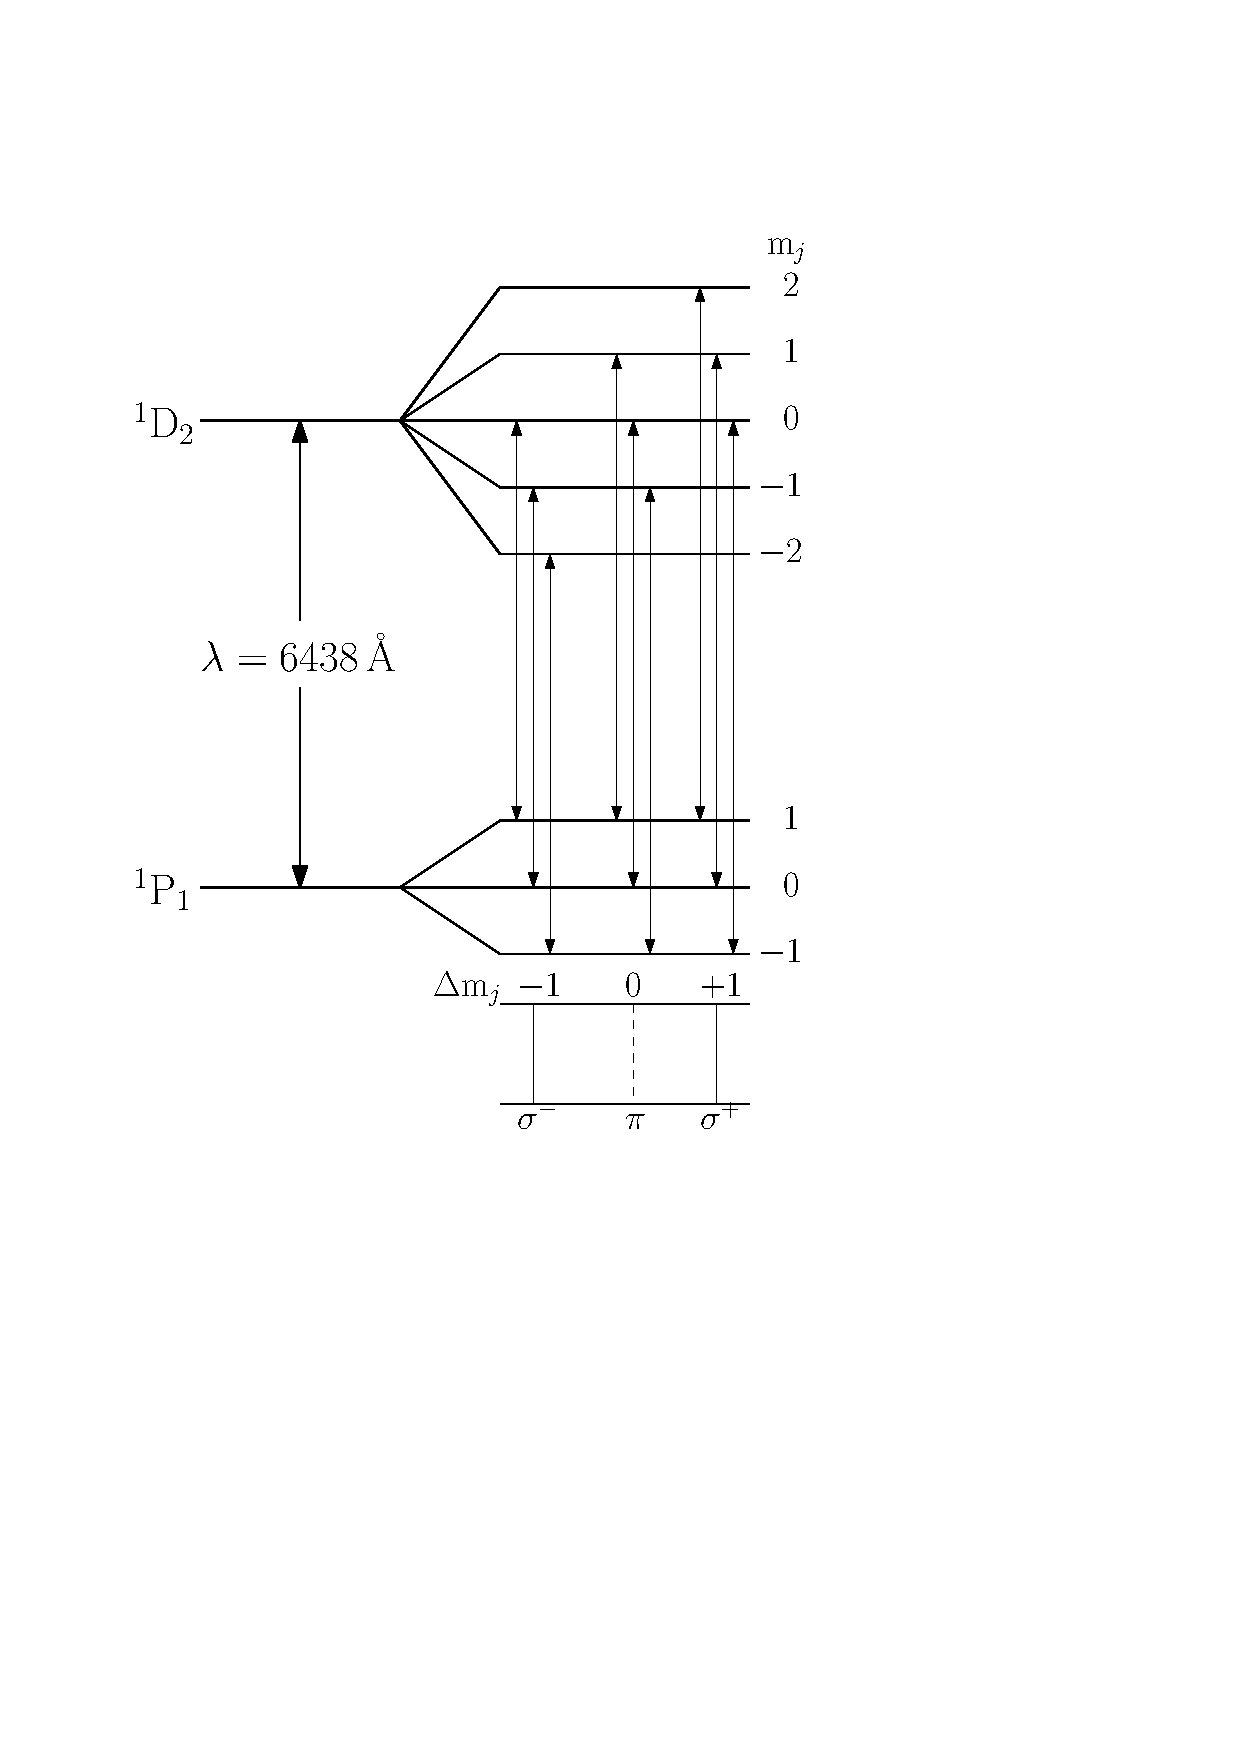
\includegraphics[width=0.4\textwidth]{./figures/termschema_cadmium.pdf}
\caption{Übergang von $^1$D$_2$ nach $^1$P$_1$ in der fünften Schale in Cadmium}
\label{fig:termschema_cadmium}
\end{figure}

Herleitung:
Ein Elektron im Atom habe den Bahndrehimpuls $\vec{\ell}$, welches im klassischen Bild einem Kreisstrom entspricht.
Dieser führt zu einem magnetischen Dipolmoment, welches gegeben ist durch:
\begin{align}
	\vec{\mu}_\ell = - \frac{\mu_\mathrm{B}}{\hbar} \vec{\ell}
\end{align}
wobei das Bohr'sche Magneton definiert ist als:
\begin{align}
	\mu_\mathrm{B} = \frac{e \hbar}{2 m_e}
\end{align}
Die potentielle Energie eines magnetischen Dipols im externen magnetischen Feld $B$ ist gegeben durch:
\begin{align}
	E_\mathrm{pot} = - \vec{\mu} \cdot \vec{B}
\end{align}
Damit kommt es zu einer Energieverschiebung $\Delta E$ der Niveaus aufgrund der potentiellen Energie des Dipols im Magnetfeld:
\begin{align}
	\Delta E = \frac{\mu_\mathrm{B}}{\hbar} \left( \vec{\ell} \cdot \vec{B} \right)
\end{align}
Wählt man $\vec{B} = (0,0,B_z)$ und dementsprechend die z-Achse als Quantisierungsachse des Drehimpulses, so folgt $\ell_z = \hbar m_\ell$ aus der magnetischen Quantenzahl $m_\ell$ und die Energieverschiebung ergibt sich zu:
\begin{align}
	\Delta E = \mu_\mathrm{B} m_\ell B_z
\end{align}
Somit wird für feste Drehimpulsquantenzahl $\ell$ die Entartung des zugehörigen Energieniveaus aufgehoben, da sich dieses in $(2\ell + 1)$ Niveaus aufspaltet.

Im Gegensatz dazu wird beim anomalen Zeeman-Effekt das magnetische Moment aufgrund des Elektronenspins beachtet.
Dies führt dazu, dass das magnetische Moment des Elektrons gegeben ist durch:
\begin{align}
\vec{\mu} = -\frac{\mu_\mathrm{B}}{\hbar} \left( \vec{l} + g_s \vec{s} \right)
\end{align}
Zur Beschreibung der Energieverschiebung ist hier die Kopplung von Spin und Bahndrehimpuls $\vec{j} = \vec{\ell} + \vec{s}$ nötig.
Da $g_s \approx 2$ ist, ist das magnetische Moment des Elektrons nicht parallel zum Gesamtdrehimpuls $\vec{j}$ und präzediert um diesen.
Daher muss ein effektives magnetisches Moment als Projektion von $\vec{\mu}$ auf $\vec{j}$ berechnet werden, was zu dem effektiven Moment:
\begin{align}
	\vec{\mu}_\mathrm{eff} = - g_j \frac{\mu_\mathrm{B}}{\hbar} \vec{j} 
\end{align}
führt.
Dabei ist der sogenannte Landé-Faktor $g_j$ abhängig von den Quantenzahlen $l,s,j$ des Zustandes.
Damit folgt analog zum normalen Zeeman-Effekt:
\begin{align}
	\Delta E = \mu_\mathrm{B} g_j m_j B_z
\end{align}


\subsubsection{Auswahlregeln}
Die Auswahlregeln für elektrische Dipolübergänge erhält man durch Berechnung der Übergangswahrscheinlichkeit vom Zustand $|i\rangle$ in den Endzustand $|f\rangle$ durch Fermi's Goldene Regel:
\begin{align}
	\lambda_{i\rightarrow f} = \frac{2 \pi}{\hbar} | \braket{f|H^\prime|i} |^2 \rho(E_\mathrm{f})
\end{align}
Dabei ist der Störhamiltonian $H^\prime$ gegeben durch die Störung der Energie aufgrund der Kopplung von einem externen elektrischen Feld $\vec{E}$ an das elektrische Dipolmoment $\vec{p}$ des Zustandes:
\begin{align}
	H^\prime = - \vec{p} \cdot \vec{E}
\end{align}
Kennzeichnend dafür, ob ein Übergang erlaubt ist, ist das jeweilige Matrixelement des Störhamiltonians.
Somit erhält man die Auswahlregeln aus den nicht verschwindenden Matrixelementen:
\begin{itemize}
	\item $\Delta n$ beliebig
	\item $\Delta \ell = \pm 1$ \quad (Drehimpulserhaltung mit $s_\mathrm{Photon} = \pm \hbar$)
	\item $\Delta s = 0$ \quad (reine Spin-Flips sind nicht möglich)
	\item $\Delta j = 0, \pm 1$, außer $j_i=0 \rightarrow j_f=0$
	\item $\Delta m_j = 0, \pm 1$
\end{itemize}
($n$: Hauptquantenzahl, $\ell$: Drehimpulsquantenzahl, $s$: Spinquantenzahl, $j$: Gesamtdrehimpulsquantenzahl, $m_j$: magnetische Quantenzahl)

Mit diesen Auswahlregeln folgen die Übergänge für Cadmium aus Abbildung \ref{fig:termschema_cadmium}.
Anzumerken ist, dass es sich dabei um den normalen Zeeman-Effekt handelt und dadurch die Aufspaltung der P-Schale ($\ell = 1$) den gleichen Abstand hat, wie die der D-Schale ($\ell = 2$).
Dadurch kommt es hier zu insgesamt drei Übergängen, mit unterschiedlichen Energien.
Im Vergleich dazu, liefert der anormaler Zeeman-Effekt mehrere Übergänge mit unterschiedlicher Energie, da sich die Energie aufgrund der Abhängigkeit vom Landé-Faktor in den jeweiligen Schalen nicht äquidistant aufspalten.

Noch erwähnen:
Elektronenkonfiguration Cad: [Kr] $4d^{10} 5s^2$ daher kein Spin (abgeschlossene Schalen)
 Abhängigkeit der Polarisation von der $m$-Quantenzahl und Einfluss auf die Linien des Zeeman-Effekts. Larmor-Frequenz $\Omega_\mathrm{L} = \frac{e B}{2 m_e}$

\subsubsection{Fabry-Pérot-Etalon}
Das Fabry-Pérot-Etalon besteht aus einer transparenten Platte, welche beidseitig von Luft umgeben ist.
Trifft elektromagnetische Welle unter dem Winkel $\alpha$ auf das Etalon, so wird diese an beiden Grenzfläche gemäß des Reflektionskoeffizienten\footnote{Der Reflektionskoeffizient beschreibt die Änderung der Amplitude der elektromagnetischen Welle bei Reflektion an der Grenzfläche. Das Verhältnis der Intensitäten ist durch den Reflektionsgrad $R = r^2$ gegeben.} $r$ reflektiert und zum Teil transmittiert.
Dies führt dazu, dass die Welle innerhalb des Etalons sehr oft hin- und her reflektiert wird und es somit auf Transmissionsseite der Platte zur Vielstrahlinterferenz der transmittierten Strahlen kommt.
Da in diesem Versuch das Fabry-Pérot-Etalon in Transmission betrieben wird, wollen wir uns auf diesen Fall beschränken.
\begin{figure}[h]
	\centering
	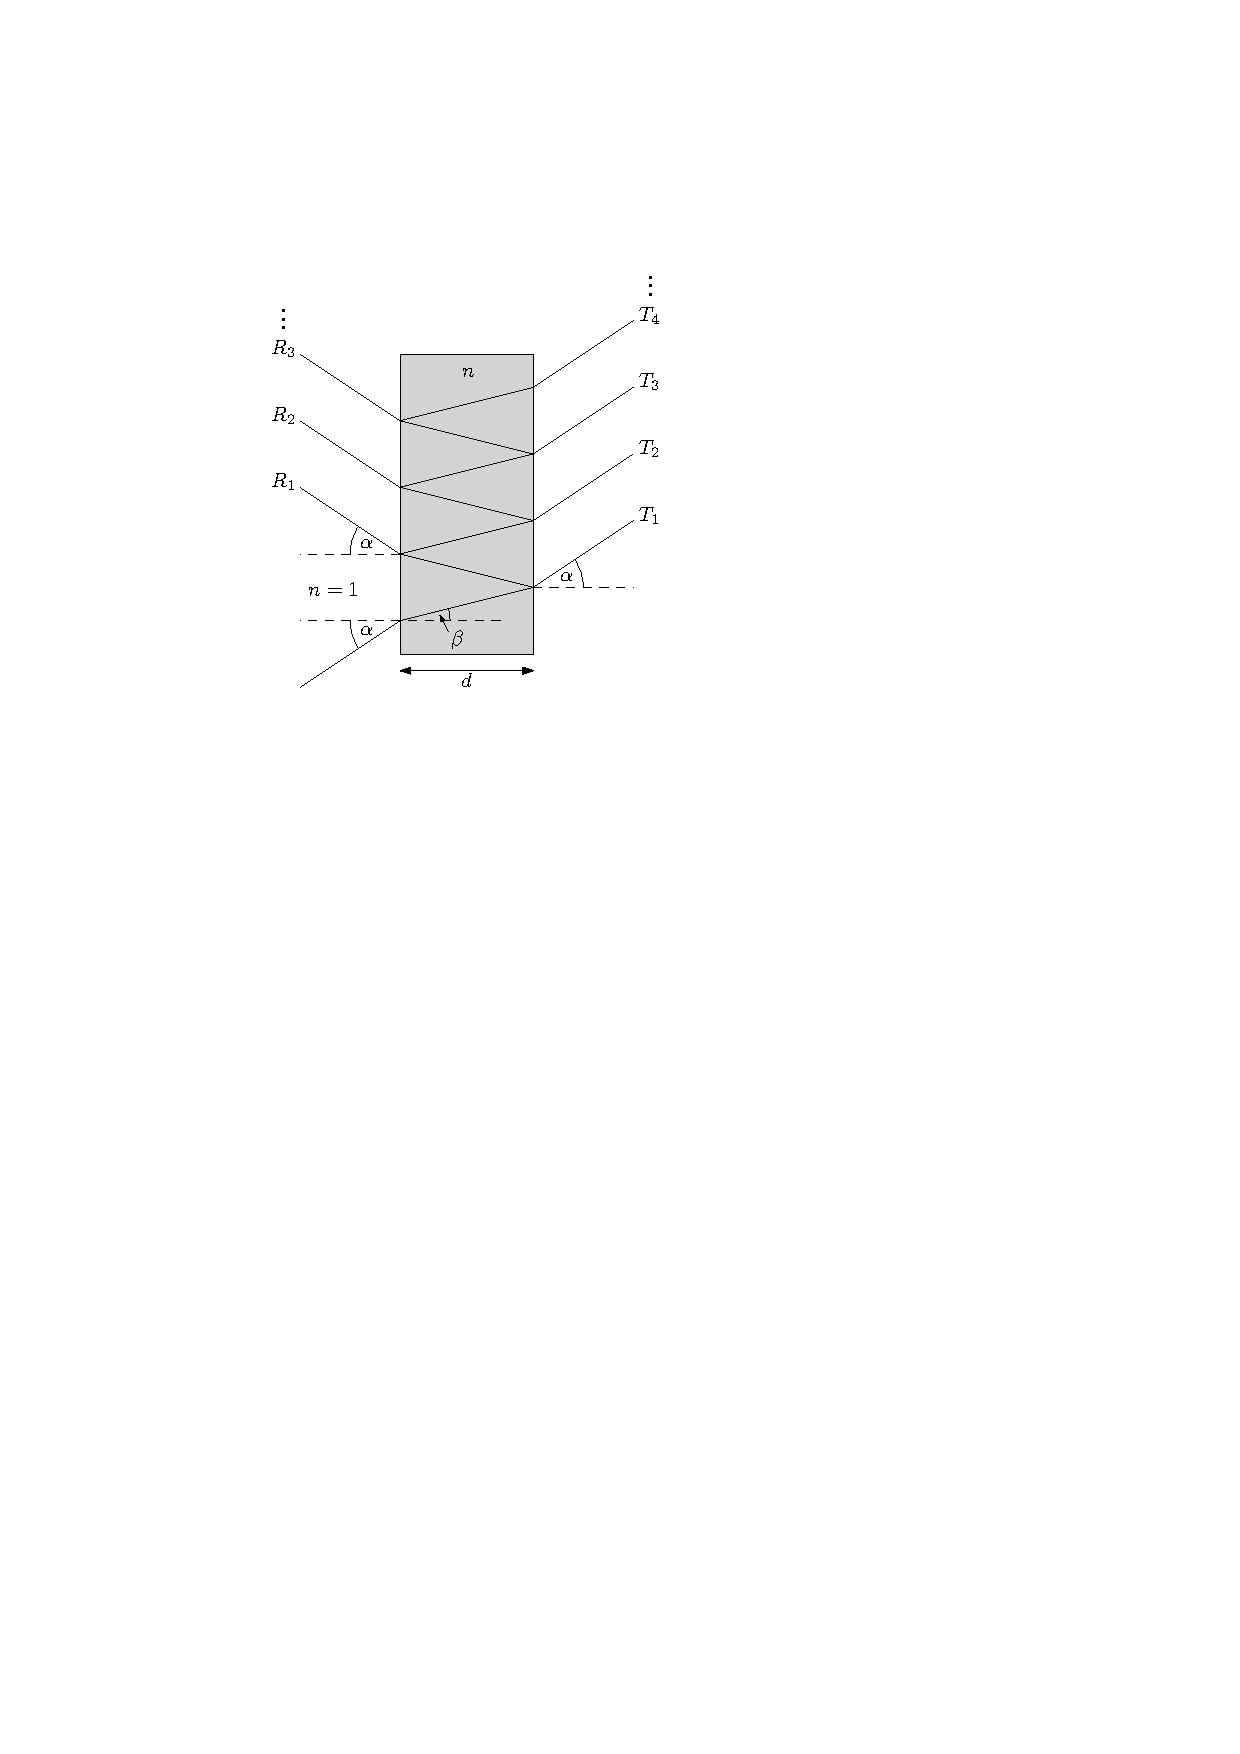
\includegraphics[width=0.6\textwidth]{./figures/fabry_perot.pdf}
	\caption{Berechnung der optischen Weglänge des Fabry-Pérot-Etalons}
	\label{fig:fabry_perot}
\end{figure}
Um die Bedingung für konstruktive Interferenz zu erhalten, muss zunächst der optische Gangunterschied zwei benachbarter Strahlen berechnet werden.
Gemäß Abbildung \ref{fig:fabry_perot} ist dieser gegeben durch:
\begin{align}
	\Delta s = \frac{2 n d}{\cos(\beta)} - 2 n d \sin(\alpha) \tan(\beta)
\end{align}
Mit dem Brechungsgesetz $\sin(\alpha) = n \sin(\beta)$ folgt:
\begin{align}
	\Delta s = 2 d \sqrt{n^2 - \sin^2(\alpha)}
\end{align}
Damit zwei benachbarte Strahlen nach der Transmission in Phase sind, muss deren Phasendifferenz $\Delta \varphi$ ein ganzzahliges Vielfaches von $2\pi$ sein:
\begin{align}
	\Delta \varphi = k \cdot \Delta s = \frac{2\pi}{\lambda} \Delta s = 2 \pi \cdot m \quad \text{für } m \in \mathbb{Z}
\end{align}
Damit ist die Bedingung für ein Maximum der Transmission:
\begin{align}
	m \lambda = 2 d \sqrt{n^2 - \sin^2(\alpha)}
	\label{eq:interferenzbedingung}
\end{align}
Führt man die Berechnung der Transmission unter Beachtung der Amplituden und Phasen der einzelnen Teilwellen durch, so erhält man für den Transmissionsgrad $T = I_\mathrm{T} / I_0$:
\begin{align}
	T = \frac{1}{1 + F \sin^2(\Delta \varphi / 2)}
\end{align}
wobei man den Finesse-Koeffizienten
\begin{align}
	F = \left( \frac{2 r}{1 - r^2} \right)^2
\end{align}
definiert.\footnote{Quelle: Vorlesung Linden}

\begin{figure}[h]
	\centering
	% GNUPLOT: LaTeX picture with Postscript
\begingroup
  \makeatletter
  \providecommand\color[2][]{%
    \GenericError{(gnuplot) \space\space\space\@spaces}{%
      Package color not loaded in conjunction with
      terminal option `colourtext'%
    }{See the gnuplot documentation for explanation.%
    }{Either use 'blacktext' in gnuplot or load the package
      color.sty in LaTeX.}%
    \renewcommand\color[2][]{}%
  }%
  \providecommand\includegraphics[2][]{%
    \GenericError{(gnuplot) \space\space\space\@spaces}{%
      Package graphicx or graphics not loaded%
    }{See the gnuplot documentation for explanation.%
    }{The gnuplot epslatex terminal needs graphicx.sty or graphics.sty.}%
    \renewcommand\includegraphics[2][]{}%
  }%
  \providecommand\rotatebox[2]{#2}%
  \@ifundefined{ifGPcolor}{%
    \newif\ifGPcolor
    \GPcolortrue
  }{}%
  \@ifundefined{ifGPblacktext}{%
    \newif\ifGPblacktext
    \GPblacktexttrue
  }{}%
  % define a \g@addto@macro without @ in the name:
  \let\gplgaddtomacro\g@addto@macro
  % define empty templates for all commands taking text:
  \gdef\gplbacktext{}%
  \gdef\gplfronttext{}%
  \makeatother
  \ifGPblacktext
    % no textcolor at all
    \def\colorrgb#1{}%
    \def\colorgray#1{}%
  \else
    % gray or color?
    \ifGPcolor
      \def\colorrgb#1{\color[rgb]{#1}}%
      \def\colorgray#1{\color[gray]{#1}}%
      \expandafter\def\csname LTw\endcsname{\color{white}}%
      \expandafter\def\csname LTb\endcsname{\color{black}}%
      \expandafter\def\csname LTa\endcsname{\color{black}}%
      \expandafter\def\csname LT0\endcsname{\color[rgb]{1,0,0}}%
      \expandafter\def\csname LT1\endcsname{\color[rgb]{0,1,0}}%
      \expandafter\def\csname LT2\endcsname{\color[rgb]{0,0,1}}%
      \expandafter\def\csname LT3\endcsname{\color[rgb]{1,0,1}}%
      \expandafter\def\csname LT4\endcsname{\color[rgb]{0,1,1}}%
      \expandafter\def\csname LT5\endcsname{\color[rgb]{1,1,0}}%
      \expandafter\def\csname LT6\endcsname{\color[rgb]{0,0,0}}%
      \expandafter\def\csname LT7\endcsname{\color[rgb]{1,0.3,0}}%
      \expandafter\def\csname LT8\endcsname{\color[rgb]{0.5,0.5,0.5}}%
    \else
      % gray
      \def\colorrgb#1{\color{black}}%
      \def\colorgray#1{\color[gray]{#1}}%
      \expandafter\def\csname LTw\endcsname{\color{white}}%
      \expandafter\def\csname LTb\endcsname{\color{black}}%
      \expandafter\def\csname LTa\endcsname{\color{black}}%
      \expandafter\def\csname LT0\endcsname{\color{black}}%
      \expandafter\def\csname LT1\endcsname{\color{black}}%
      \expandafter\def\csname LT2\endcsname{\color{black}}%
      \expandafter\def\csname LT3\endcsname{\color{black}}%
      \expandafter\def\csname LT4\endcsname{\color{black}}%
      \expandafter\def\csname LT5\endcsname{\color{black}}%
      \expandafter\def\csname LT6\endcsname{\color{black}}%
      \expandafter\def\csname LT7\endcsname{\color{black}}%
      \expandafter\def\csname LT8\endcsname{\color{black}}%
    \fi
  \fi
  \setlength{\unitlength}{0.0500bp}%
  \begin{picture}(7200.00,5040.00)%
    \gplgaddtomacro\gplbacktext{%
      \csname LTb\endcsname%
      \put(946,374){\makebox(0,0)[r]{\strut{} 0}}%
      \put(946,1254){\makebox(0,0)[r]{\strut{} 0.2}}%
      \put(946,2134){\makebox(0,0)[r]{\strut{} 0.4}}%
      \put(946,3015){\makebox(0,0)[r]{\strut{} 0.6}}%
      \put(946,3895){\makebox(0,0)[r]{\strut{} 0.8}}%
      \put(946,4775){\makebox(0,0)[r]{\strut{} 1}}%
      \put(176,2574){\rotatebox{-270}{\makebox(0,0){\strut{}Transmissionsgrad}}}%
      \put(3940,154){\makebox(0,0){\strut{}Wellenl\"ange $\lambda$}}%
      \put(3940,4665){\makebox(0,0){\strut{}}}%
    }%
    \gplgaddtomacro\gplfronttext{%
    }%
    \gplbacktext
    \put(0,0){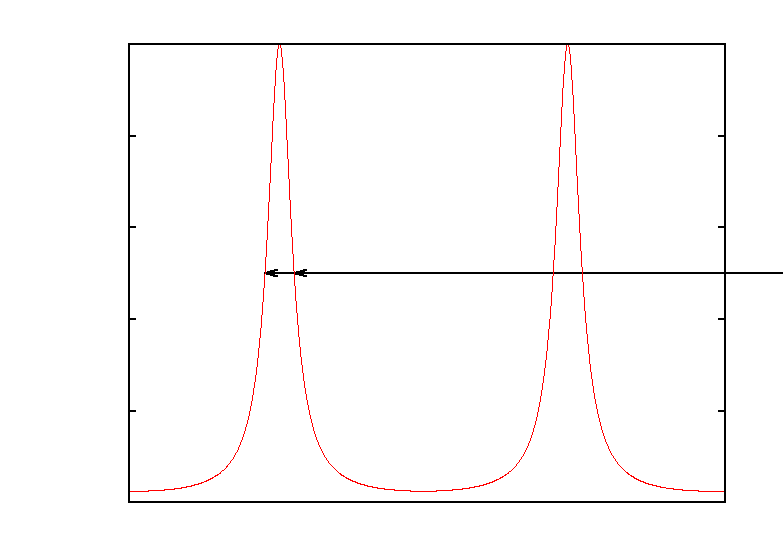
\includegraphics{./fabry_perot_transmission}}%
    \gplfronttext
  \end{picture}%
\endgroup

	\caption{UNTERSCHRIFT}
	\label{fig:fabry_transmission}
\end{figure}

Zwei wichtige Kenngrößen des Fabry-Pérot-Etalons sind die Halbwertsbreite des Transmissionsmaximums $\delta \lambda$, sowie der freie Spektralbereich $\Delta \lambda$, welcher als Abstand zweier Transmissionsmaxima definiert ist.
Mit diesen zwei Größen definiert man die Finesse $\mathcal{F}$ des Etalons\footnote{Quelle!}:
\begin{align}
	\mathcal{F} = \frac{\Delta \lambda}{\delta \lambda} = \frac{\pi \sqrt{F}}{2} = \frac{\pi r}{1 - r^2}
\end{align}

Das Auflösungsvermögen ist definiert als das Verhältnis der Wellenlänge $\lambda$ zur Wellenlängendifferenz von zwei gerade noch auflösbaren Linien.
Gerade noch auflösbar heißt dabei, dass das Rayleigh-Kriterium erfüllt ist, welches besagt, dass der Abstand der beiden Intensitätsmaxima genau der Halbwertsbreite des Intensitätsverlaufs entspricht.
Damit folgt mit der Halbwertsbreite $\delta \lambda$ der Maxima des Fabry-Pérot-Etalons:\footnote{Quelle: Hecht}
\begin{align}
	\mathcal{R} = \frac{\lambda}{\delta \lambda} = \mathcal{F} \cdot m
\end{align}

\subsubsection{Natürliche Linienbreite und Linienverbreiterung}
Aufgrund der Heisenberg'schen Unschärferelation führt die endlichen Lebensdauer $\tau$ angeregter Zustände zu einer Energieunschärfe $\Gamma$ bei der Relaxation des Zustandes.
Die Energieunschärfe ist gegeben durch:
\begin{align}
	\Gamma = \frac{\hbar}{\tau}
\end{align}
Diese Energieunschärfe hat ein Lorentz-Profil.

Darüber hinaus kommt es zur Dopplerverbreiterung aufgrund der thermischen Bewegung der angeregten Atome.
Die Geschwindigkeitsverteilung der Atome in Beobachtungsrichtung ist gaußförmig um Null, sodass auch die Dopplerverbreitung ein gaußförmiges Profil hat.

Die Kombination von natürlicher Linienbreite (Lorentz) und Dopplerverbreiterung (Gauß) führt (Faltung) zu einem sogenannten Voigt-Profil.

\subsubsection{$\frac{\lambda}{4}$-Platte}
Eine $\lambda/4$-Platte besteht aus doppelbrechendem Material dessen optische Achse parallel zu den Grenzflächen ausgerichtet ist.
Im Zuge dieser Erklärung wollen wir davon ausgehen, dass die optische Achse mit der y-Achse übereinstimmt.
Dann unterscheidet sich der Brechungsindex in x-Richtung $n_x$ von dem in y-Richtung $n_y$, was dazu führt, dass Phasendifferenzen zwischen den x- und y-polarisierten Anteilen des Lichts entstehen.
Die Phasendifferenz ist gegeben durch:
\begin{align}
	\Delta \varphi = \frac{2 \pi}{\lambda} d (n_y - n_x)
\end{align}
wobei $d$ die Dicke der Platte ist.
Bei einer $\lambda / 4$-Platte wird die Dicke $d$ so gewählt, dass:
\begin{align}
	d (n_y - n_x) = \frac{\lambda}{4}
\end{align}
ist, was zu einer Phasendifferenz $\Delta \varphi = \pm \pi / 2$ führt.

Diese Phasenverschiebung führt dazu, dass um $\pm\SI{45}{\degree}$ (andere Winkel führen zu elliptischer Polarisation) gegen die optische Achse der $\lambda/4$-Platte verdrehtes linear polarisiertes Licht hinter der Platte zirkular polarisiert ist.
Umgekehrt wird zirkular polarisiertes Licht durch die Platte in zwei ebenfalls um $\pm\SI{45}{\degree}$ gegen die optische Achse verkippte linear polarisierte Wellen aufgespalten.
Diese Eigenschaften der $\lambda/4$-Platte ermöglichen es unter Zunahme eines Polarisationsfilters Licht auf zirkulare Polarisation zu untersuchen.


\subsubsection{Hall-Sonde}
\begin{figure}
	\centering
	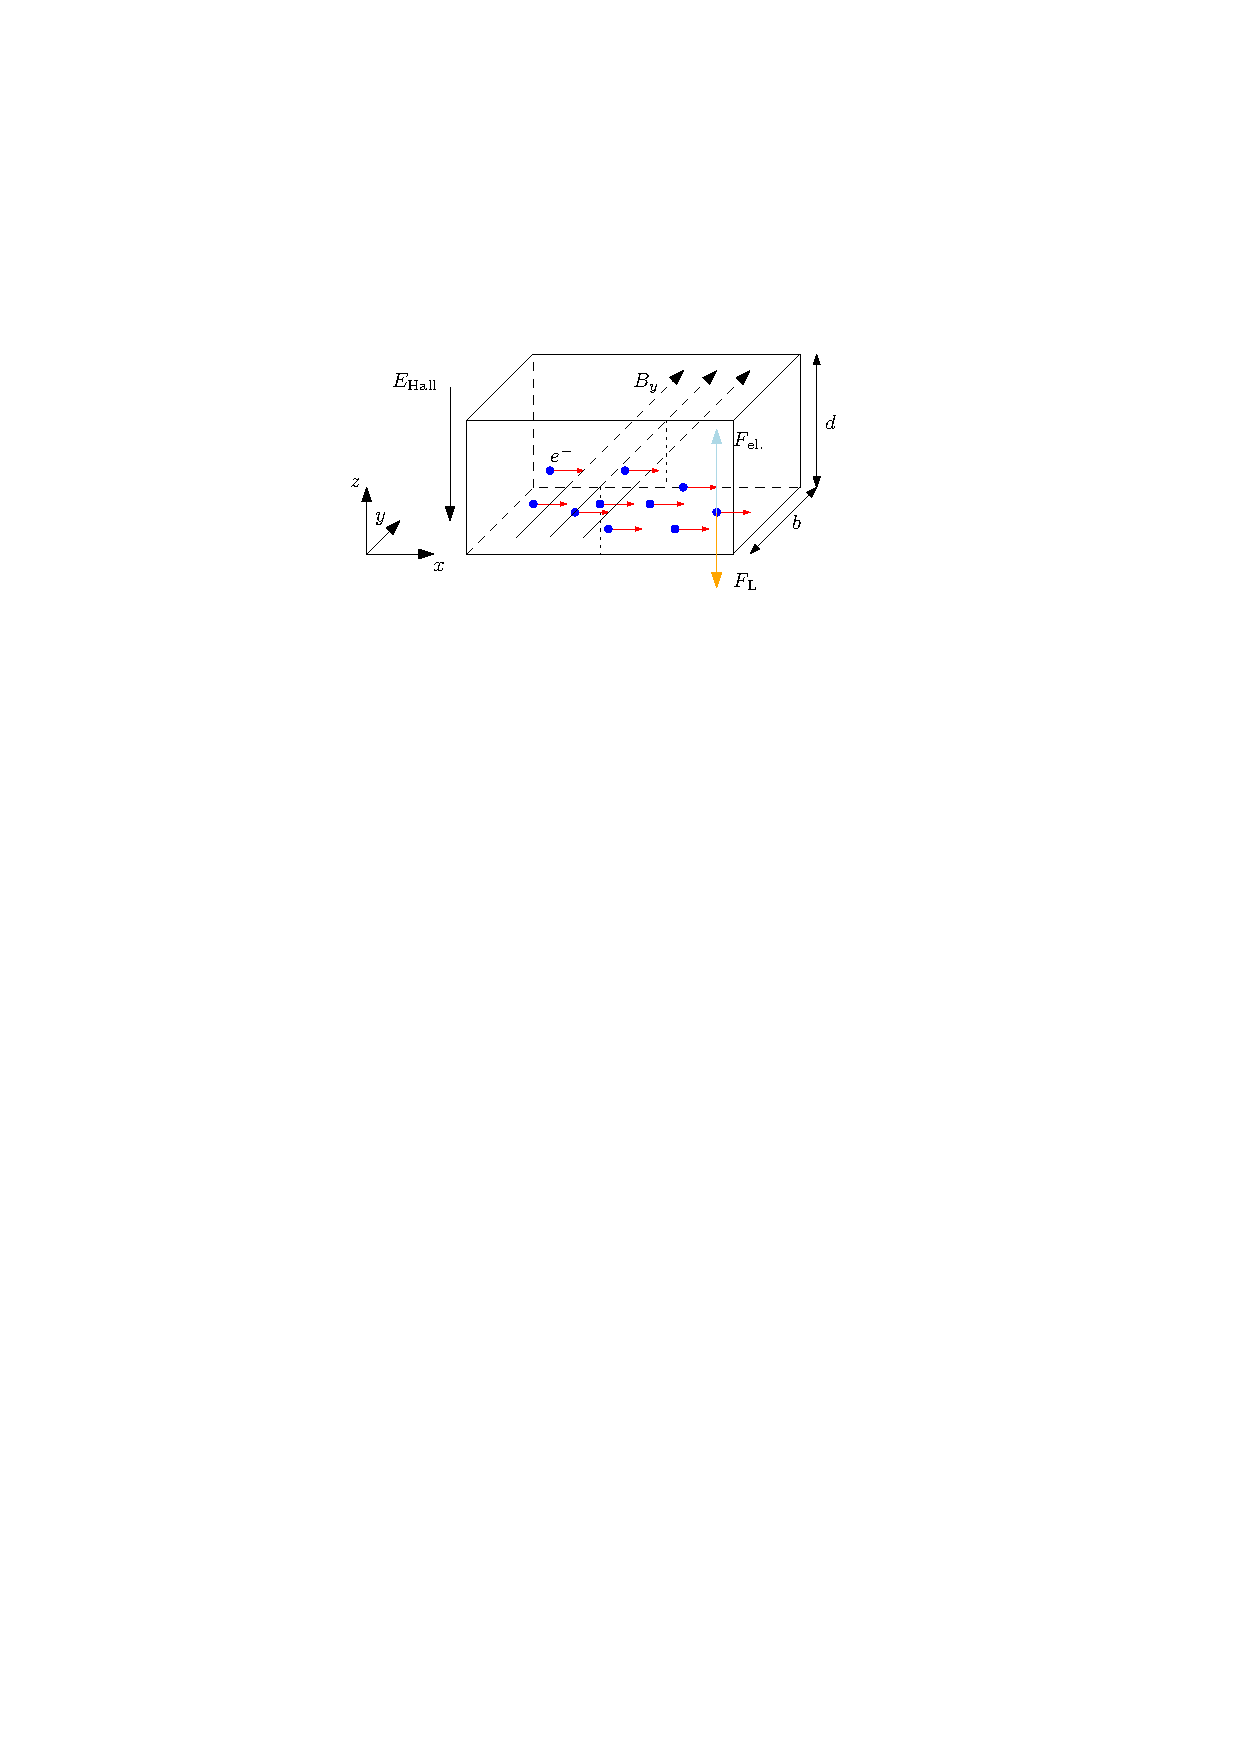
\includegraphics[width=0.7\textwidth]{./figures/hall_effekt.pdf}
	\caption{Zur Herleitung des Hall-Effekts}
	\label{fig:hall_effekt}
\end{figure}
In Hall-Sonden wird der Hall-Effekt ausgenutzt, welcher besagt, dass an einem stromdurchflossenen Leiter im Magnetfeld $B_y$ eine Spannung $U_\mathrm{Hall}$ über den Seitenflächen des Leitermaterials entsteht, die aufgrund der Lorentzkraft auf die bewegten Ladungsträger entsteht.
Die Ladungsträger werden durch die Lorentzkraft soweit ausgelenkt, bis das durch die Auslenkung entstandene elektrische Feld $E_\mathrm{Hall}$ die Lorentzkraft kompensiert:
\begin{align}
	e E_\mathrm{Hall} = e v_x B_y
	\label{eq:kompensation}
\end{align}
Dabei ist die an den Stirnflächen mit Abstand $d$ anliegende Spannung gegeben durch $E_\mathrm{Hall} = U_\mathrm{Hall} / d$, womit aus Gleichung \ref{eq:kompensation} folgt:
\begin{align}
	U_\mathrm{Hall} = d v_x B_y
\end{align}
Die Geschwindigkeit der Ladungsträger $v_x$ lässt sich nun über die Stromdichte $j_x = e n v_x = I/A$ ausdrücken, wobei $A = d \cdot b$ die Querschnittsfläche des Leiters ist.
Damit folgt die Hall-Spannung:
\begin{align}
	U_\mathrm{Hall} = \frac{I B_y}{b\, n\, e}
\end{align}
Somit ist die Hall-Spannung proportional zum Magnetfeld $B_y$ und kann damit zur Messung desselben verwendet werden.
Praktisch werden, um bei kleinem Strom $I$ große Spannung zu erzielen, Halbleitermaterialien verwendet, da diese eine kleine Ladungsträgerdichte $n$ aufweisen.


\subsection{Franck-Hertz-Versuch}

Der Franck-Hertz-Versuch wurde um 1914 von James Franck und Gustav Hertz \cite{demtroeder3} durchgeführt und demonstrierte die Wichtigkeit der Energiequantelung bei Stoßprozessen.
In dem Versuch wird eine mit Quecksilberdampf bei Unterdruck (ca. \SI{e-2}{\milli\bar}) gefüllte Elektronenröhre genutzt, bei der zwischen Kathode und Anode ein Gitter eingebaut ist, und die variable Beschleunigungsspannung $U$ zwischen Kathode und Gitter anliegt.
Zwischen diesem und der Anode wird eine konstante Gegenspannung $\Delta U$ angelegt.
\begin{figure}[h]
\centering
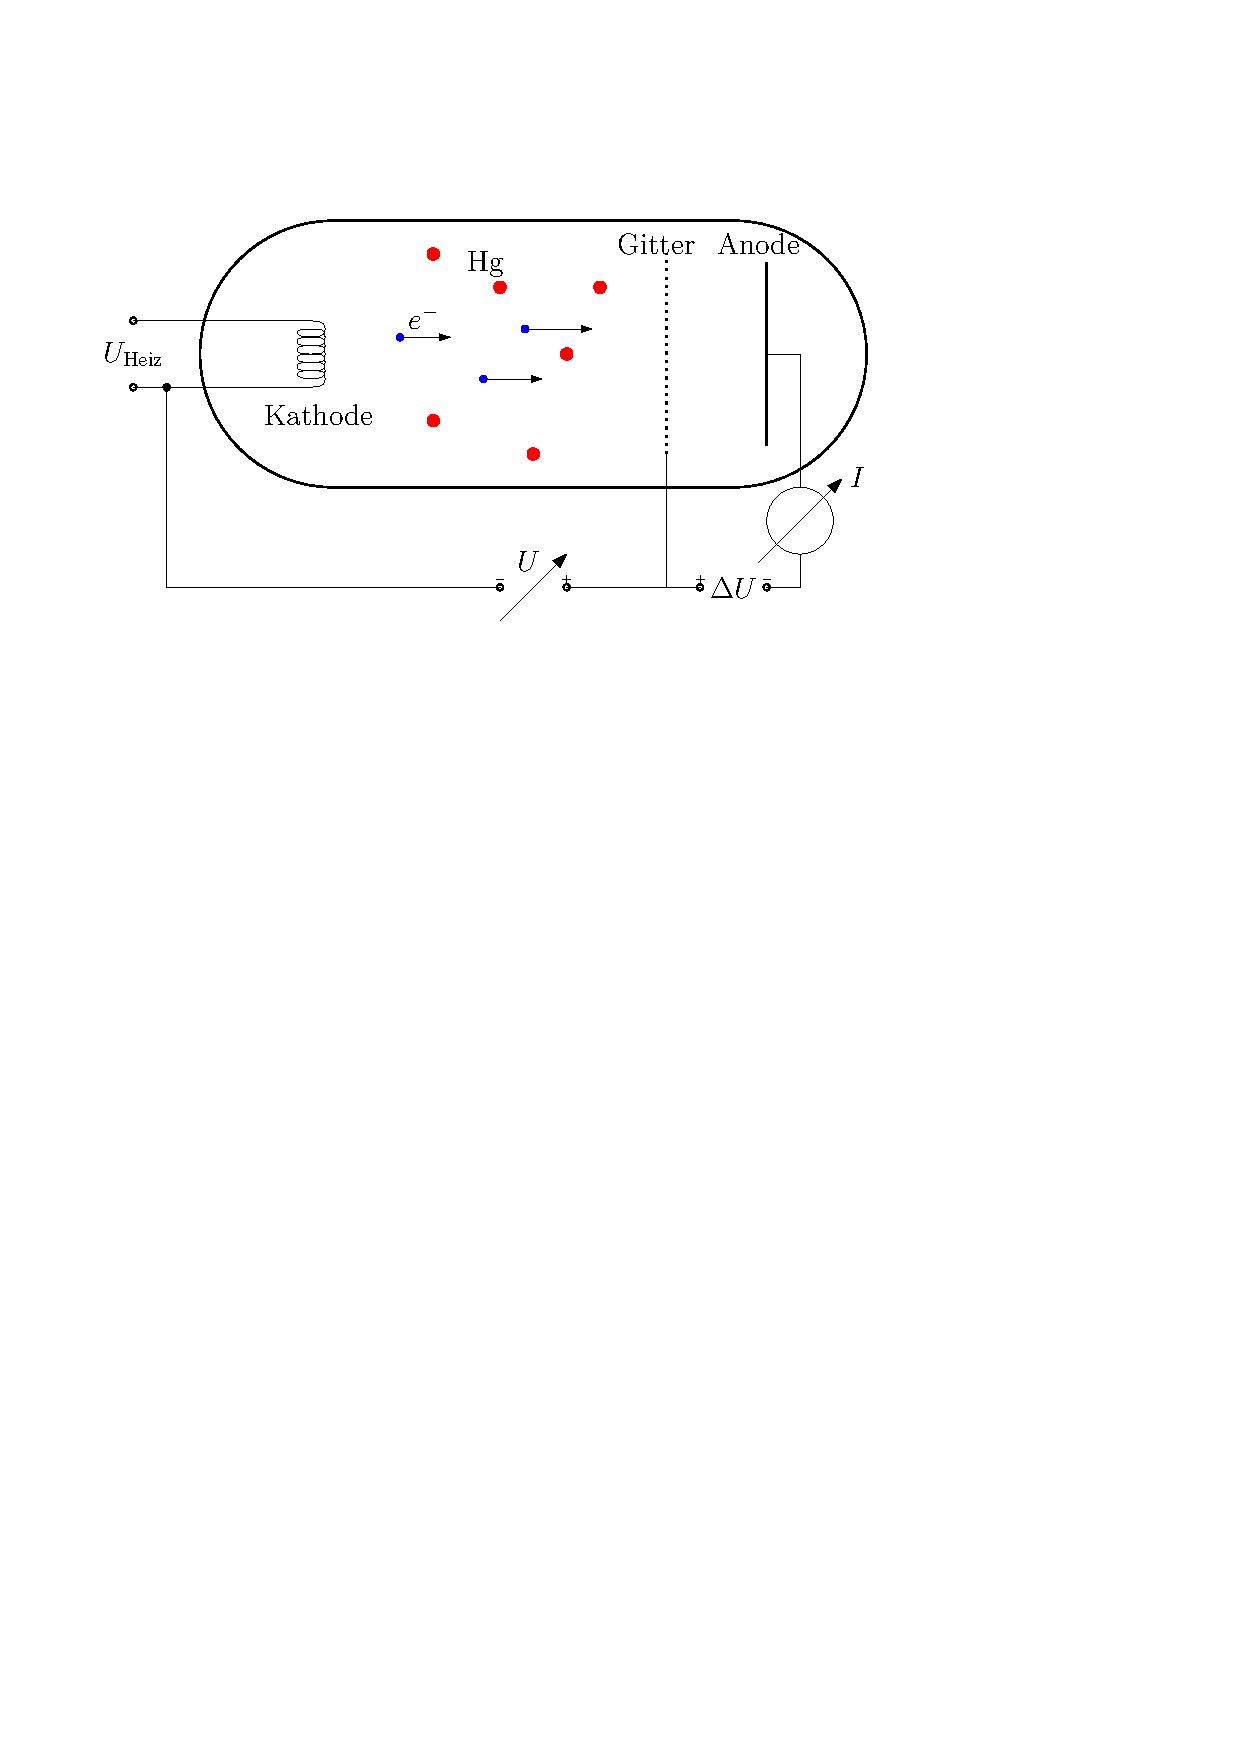
\includegraphics[width=0.7\textwidth]{./figures/franck-hertz_aufbau.pdf}
\caption{Aufbau des Franck-Hertz-Versuches}
\label{fig:franck-hertz_aufbau}
\end{figure}
Durch den glühlektrischen Effekt treten an der Kathode bei Anlegen einer hohen Spannung Elektronen aus.
Dies geschieht dadurch, dass die Elektronen im Draht durch die hohe Spannung angeregt werden und die (vom Material abhängige) Austrittsarbeit überwinden.
Die Stromdichte der aus einem Metall austretenden Elektronen wird beschrieben durch die \textbf{Richardson-Gleichung} \cite{np_richardson}:
\begin{align*}
j=AT^2\cdot \exp\left({-\dfrac{\omega}{\mathrm{k_B}T}}\right)
\end{align*}
Dabei ist $T$ die absolute Temperatur, $\mathrm{k_B}$ die Boltzmann-Konstante und $A$ und $\omega$ materialabhängige Konstanten.
Die so ausgetretenen Elektronen werden von dem äußeren anliegenden Feld durch die Beschleunigungsspannung zum Gitter hin beschleunigt und erreichen dabei die Energie $eU$.
Durch die zwischen Gitter und Anode anliegende Gegenspannung werden die Elektronen nach Passieren des Gitters abgebremst und nur solche mit Energien größer als $e\Delta U$ erreichen die Anode.
Der Aufbau bildet so ein Triodensystem.
\begin{figure}[h]
\centering
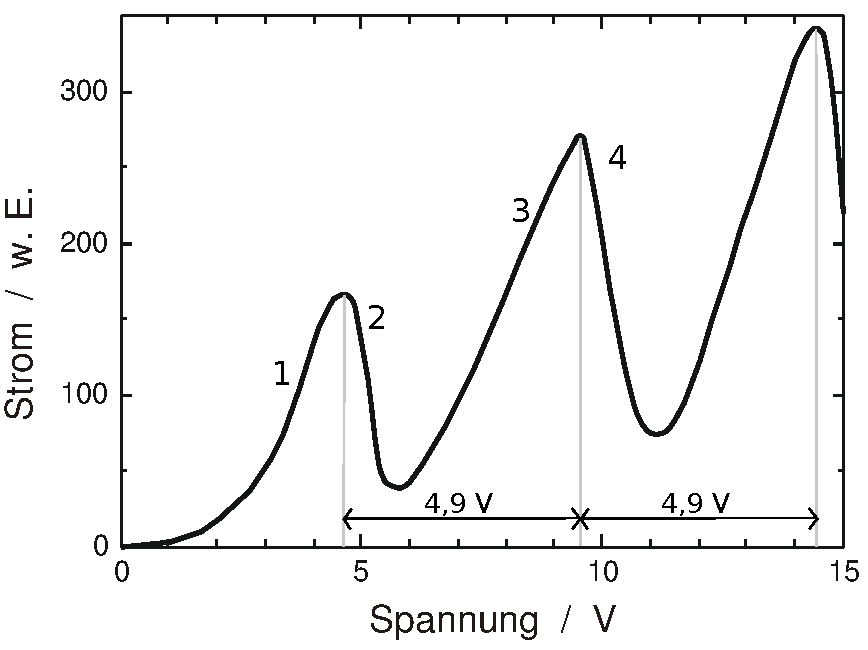
\includegraphics[width=0.5\textwidth]{./figures/franck-hertz_ergebnis.pdf}
\caption{Anodenstrom beim Franck-Hertz-Versuch mit Quecksilber, aufgetragen gegen die Beschleunigungsspannung; nach Originaldaten von Franck und Hertz. Quelle: \url{http://upload.wikimedia.org/wikipedia/commons/5/50/Franck-Hertz_de.svg} (abgerufen am 14.11.2014)}
\label{fig:franck-hertz_ergebnis}
\end{figure}
Bei der Durchführung des Versuches stellte man fest, dass der Anodenstrom sich wie in Abbildung \ref{fig:franck-hertz_ergebnis} verhält.
Man sieht dabei, dass in Abständen von \SI{4.9}{\volt} (der Wert gilt nur für Quecksilber) der Strom stark einbricht und ab den Minima jeweils einer Diodencharakteristik folgt \cite{demtroeder3}.
Der Grund dafür ist, dass die Elektronen auf der Beschleunigungsstrecke inelastische Stöße mit den Quecksilberatomen ausführen und diese dadurch anregen.
Die dabei an das Quecksilber abgegebene Energie steht den Elektronen nicht mehr zur Verfügung, um die Anode zu erreichen, der Strom bricht ein. 
Der Abstand der Maxima entspricht dabei genau der Anregungsenergie der Quecksilberatome.
In diesem Versuch soll die Übergangsenergie der Resonanzlinien von Quecksilber bestimmt werden. (ist das gleich der Anregungsenergie?)

\subsubsection{Röhrenelektronik}

\begin{itemize}
\item Glühemission
\item Raumladung
\item Elektronenbewegung in Triodensystem
\end{itemize}

\subsubsection{Thermodynamik und Stoßprozesse}

\begin{itemize}
\item Gaskinetik
\item Zwei-Phasen-System
\item (in-)elastische Stöße
\item mittlere freie Weglänge
\item Stoßquerschnitt
\item Gegenfeldmethode
\end{itemize}

\subsubsection{Quecksilberatom}

\begin{itemize}
\item LS- / jj-Kopplung
\item Termschema
\item Auswahlregeln
\item Resonanzabsorption
\end{itemize}

\section{Zeemann-Effekt}
Hier kurze Einführung (was wird gemacht)

\subsection{Versuchsdurchführung}

\subsubsection{Versuchsaufbau und Justage}
\begin{figure}[h]
	\centering
	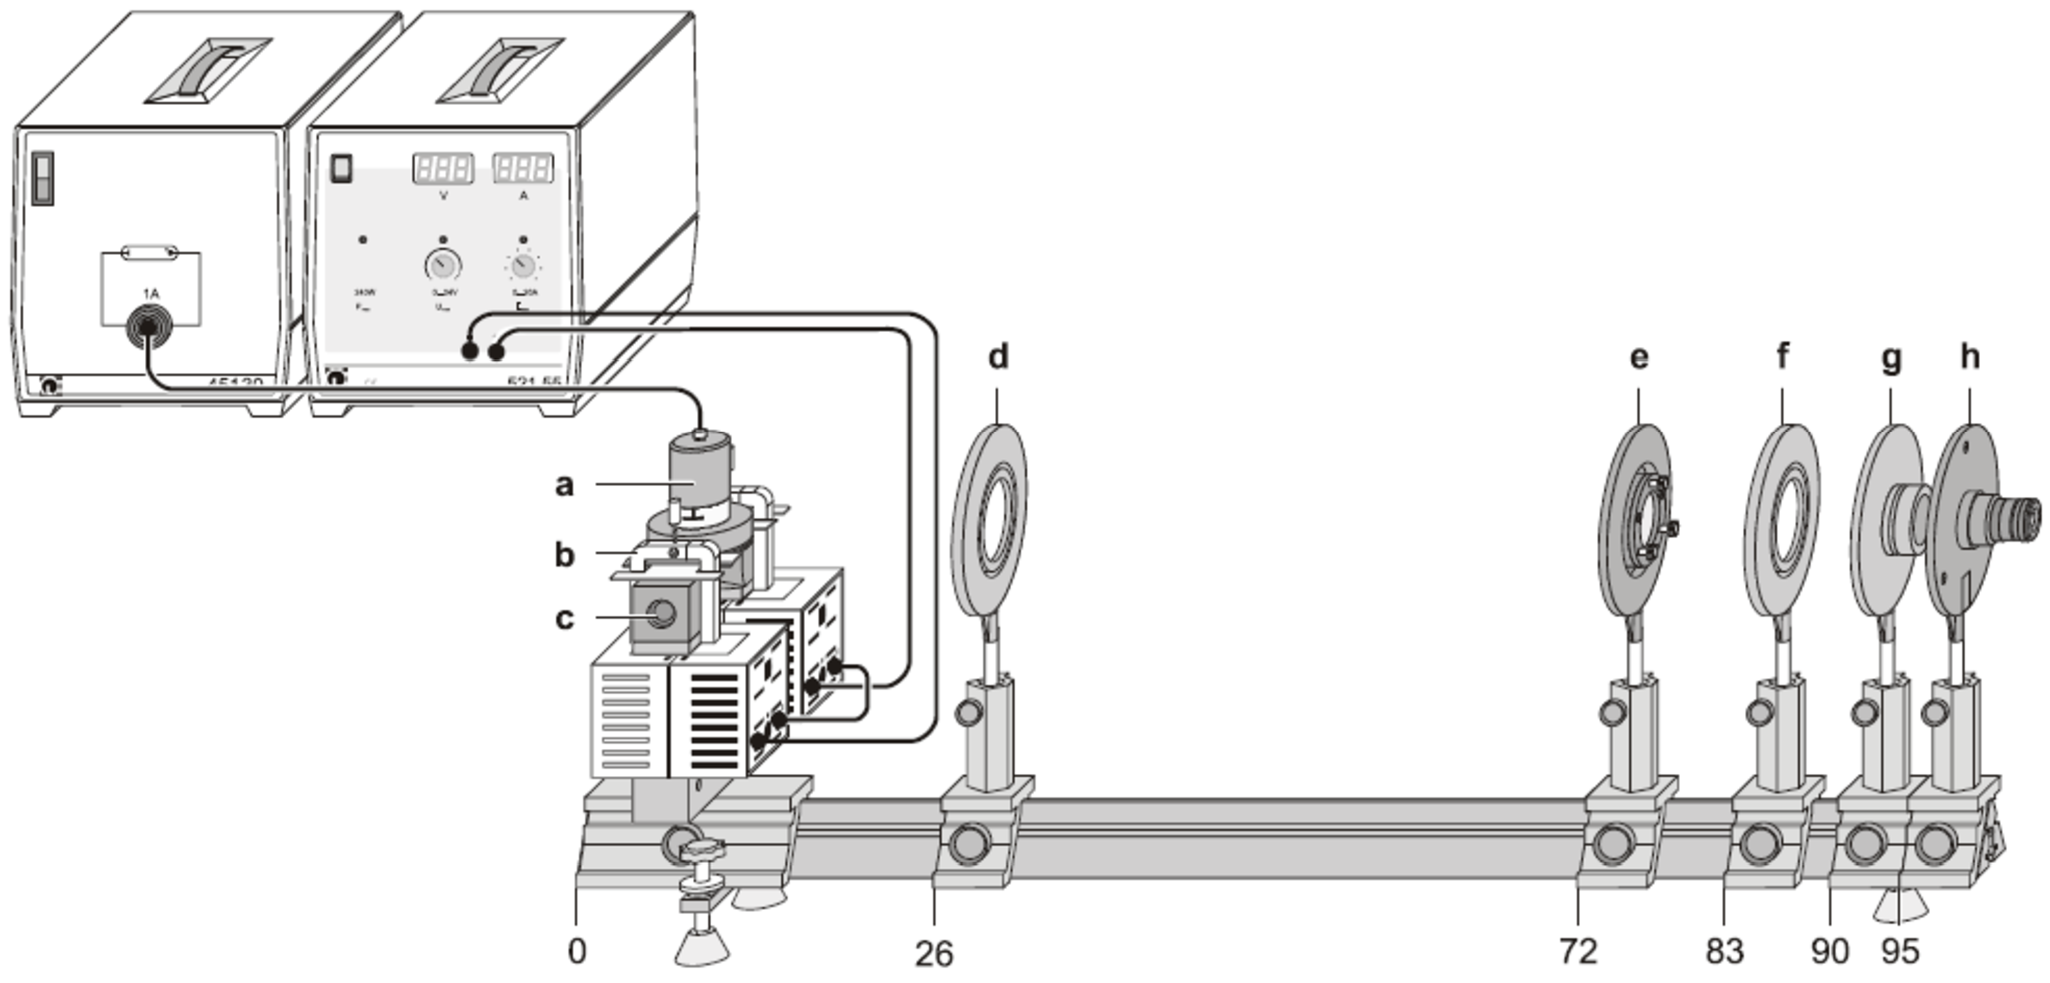
\includegraphics[width=1.0\textwidth]{./figures/aufbau_zeeman.pdf}
	\caption{Aufbau Zeeman transversal. LD Didactic. \textbf{a}) Cadmiumlampe \textbf{b}) Klammern \textbf{c}) Polschuhe \textbf{d}) Kondensor $f=\SI{150}{\milli\metre}$ \textbf{e}) Fabry-Pérot-Etalon \textbf{f}) Abbildungslinse $f=\SI{150}{\milli\metre}$ \textbf{g}) Interferenzfilter \textbf{h}) Okular }
	\label{fig:aufbau_zeeman}
\end{figure}

Zur Beobachtung der Energieaufspaltung des Zeeman-Effekts bauen wir die Apperatur wie in Abbildung \ref{fig:aufbau_zeeman} auf.
Dazu führen wir zunächst die Cadmium-Lampe zwischen die Polschuhe, welche mit dem Kern der beiden Magnetspulen verbunden sind.
Dabei achten wir darauf, dass die Verbindung der Lampe mit dem Netzgerät, sowie die Abschmelzstelle des Lampenkolbens nicht im Strahlengang liegt.
(Knebelschrauben erwähnen?)

Nun bauen wir die optischen Elemente (\textbf{d} -- \textbf{h}) ein.
Zur Justage der Apperatur halten wir vor das Fabry-Pérot-Etalon ein Blatt Papier und stellen die Kondensorlinse so ein, dass das Etalon komplett ausgeleuchtet wird.
Direkt vor das Okular mit Strichskala stellen wir den Interferenzfilter mit Mittelwellenlänge $\lambda = \SI{643,8 +- 2}{\nano\metre}$ um das sichtbare Raumlicht zu minimieren.
Anschließend stellen wir die Abbildungslinse (\textbf{f}) so ein, dass das Etalon scharf durch das Okular abgebildet wird.
Da das Zentrum des Ringsystems nicht mit der Strichskala des Okulars übereinstimmt, kippen wir das Fabry-Pérot-Etalon mit den daran angebrachten Stellschrauben bis dies der Fall ist.

\subsubsection{Beobachtung der Aufspaltung in transversaler Konfiguration}

\subsubsection{Beobachtung der Aufspaltung in longitudinaler Konfiguration}




\subsubsection{Messung des Zeeman-Effekts}



\subsection{Messdaten}
\FloatBarrier

\begin{figure}[h]
\centering
% GNUPLOT: LaTeX picture with Postscript
\begingroup
  \makeatletter
  \providecommand\color[2][]{%
    \GenericError{(gnuplot) \space\space\space\@spaces}{%
      Package color not loaded in conjunction with
      terminal option `colourtext'%
    }{See the gnuplot documentation for explanation.%
    }{Either use 'blacktext' in gnuplot or load the package
      color.sty in LaTeX.}%
    \renewcommand\color[2][]{}%
  }%
  \providecommand\includegraphics[2][]{%
    \GenericError{(gnuplot) \space\space\space\@spaces}{%
      Package graphicx or graphics not loaded%
    }{See the gnuplot documentation for explanation.%
    }{The gnuplot epslatex terminal needs graphicx.sty or graphics.sty.}%
    \renewcommand\includegraphics[2][]{}%
  }%
  \providecommand\rotatebox[2]{#2}%
  \@ifundefined{ifGPcolor}{%
    \newif\ifGPcolor
    \GPcolortrue
  }{}%
  \@ifundefined{ifGPblacktext}{%
    \newif\ifGPblacktext
    \GPblacktexttrue
  }{}%
  % define a \g@addto@macro without @ in the name:
  \let\gplgaddtomacro\g@addto@macro
  % define empty templates for all commands taking text:
  \gdef\gplbacktext{}%
  \gdef\gplfronttext{}%
  \makeatother
  \ifGPblacktext
    % no textcolor at all
    \def\colorrgb#1{}%
    \def\colorgray#1{}%
  \else
    % gray or color?
    \ifGPcolor
      \def\colorrgb#1{\color[rgb]{#1}}%
      \def\colorgray#1{\color[gray]{#1}}%
      \expandafter\def\csname LTw\endcsname{\color{white}}%
      \expandafter\def\csname LTb\endcsname{\color{black}}%
      \expandafter\def\csname LTa\endcsname{\color{black}}%
      \expandafter\def\csname LT0\endcsname{\color[rgb]{1,0,0}}%
      \expandafter\def\csname LT1\endcsname{\color[rgb]{0,1,0}}%
      \expandafter\def\csname LT2\endcsname{\color[rgb]{0,0,1}}%
      \expandafter\def\csname LT3\endcsname{\color[rgb]{1,0,1}}%
      \expandafter\def\csname LT4\endcsname{\color[rgb]{0,1,1}}%
      \expandafter\def\csname LT5\endcsname{\color[rgb]{1,1,0}}%
      \expandafter\def\csname LT6\endcsname{\color[rgb]{0,0,0}}%
      \expandafter\def\csname LT7\endcsname{\color[rgb]{1,0.3,0}}%
      \expandafter\def\csname LT8\endcsname{\color[rgb]{0.5,0.5,0.5}}%
    \else
      % gray
      \def\colorrgb#1{\color{black}}%
      \def\colorgray#1{\color[gray]{#1}}%
      \expandafter\def\csname LTw\endcsname{\color{white}}%
      \expandafter\def\csname LTb\endcsname{\color{black}}%
      \expandafter\def\csname LTa\endcsname{\color{black}}%
      \expandafter\def\csname LT0\endcsname{\color{black}}%
      \expandafter\def\csname LT1\endcsname{\color{black}}%
      \expandafter\def\csname LT2\endcsname{\color{black}}%
      \expandafter\def\csname LT3\endcsname{\color{black}}%
      \expandafter\def\csname LT4\endcsname{\color{black}}%
      \expandafter\def\csname LT5\endcsname{\color{black}}%
      \expandafter\def\csname LT6\endcsname{\color{black}}%
      \expandafter\def\csname LT7\endcsname{\color{black}}%
      \expandafter\def\csname LT8\endcsname{\color{black}}%
    \fi
  \fi
  \setlength{\unitlength}{0.0500bp}%
  \begin{picture}(7200.00,5760.00)%
    \gplgaddtomacro\gplbacktext{%
      \csname LTb\endcsname%
      \put(946,704){\makebox(0,0)[r]{\strut{} 0}}%
      \csname LTb\endcsname%
      \put(946,1388){\makebox(0,0)[r]{\strut{} 100}}%
      \csname LTb\endcsname%
      \put(946,2073){\makebox(0,0)[r]{\strut{} 200}}%
      \csname LTb\endcsname%
      \put(946,2757){\makebox(0,0)[r]{\strut{} 300}}%
      \csname LTb\endcsname%
      \put(946,3442){\makebox(0,0)[r]{\strut{} 400}}%
      \csname LTb\endcsname%
      \put(946,4126){\makebox(0,0)[r]{\strut{} 500}}%
      \csname LTb\endcsname%
      \put(946,4811){\makebox(0,0)[r]{\strut{} 600}}%
      \csname LTb\endcsname%
      \put(946,5495){\makebox(0,0)[r]{\strut{} 700}}%
      \csname LTb\endcsname%
      \put(1078,484){\makebox(0,0){\strut{} 0}}%
      \csname LTb\endcsname%
      \put(1651,484){\makebox(0,0){\strut{} 1}}%
      \csname LTb\endcsname%
      \put(2223,484){\makebox(0,0){\strut{} 2}}%
      \csname LTb\endcsname%
      \put(2796,484){\makebox(0,0){\strut{} 3}}%
      \csname LTb\endcsname%
      \put(3368,484){\makebox(0,0){\strut{} 4}}%
      \csname LTb\endcsname%
      \put(3941,484){\makebox(0,0){\strut{} 5}}%
      \csname LTb\endcsname%
      \put(4513,484){\makebox(0,0){\strut{} 6}}%
      \csname LTb\endcsname%
      \put(5086,484){\makebox(0,0){\strut{} 7}}%
      \csname LTb\endcsname%
      \put(5658,484){\makebox(0,0){\strut{} 8}}%
      \csname LTb\endcsname%
      \put(6231,484){\makebox(0,0){\strut{} 9}}%
      \csname LTb\endcsname%
      \put(6803,484){\makebox(0,0){\strut{} 10}}%
      \put(176,3099){\rotatebox{-270}{\makebox(0,0){\strut{}Magnetfeld $B$ im Luftspalt / \si{\milli\tesla}}}}%
      \put(3940,154){\makebox(0,0){\strut{}Spulenstrom $I$ / \si{\ampere}}}%
      \put(3940,5385){\makebox(0,0){\strut{}}}%
    }%
    \gplgaddtomacro\gplfronttext{%
      \csname LTb\endcsname%
      \put(2662,5322){\makebox(0,0)[r]{\strut{}Messwerte}}%
      \csname LTb\endcsname%
      \put(2662,5102){\makebox(0,0)[r]{\strut{}Fitfunktion}}%
    }%
    \gplbacktext
    \put(0,0){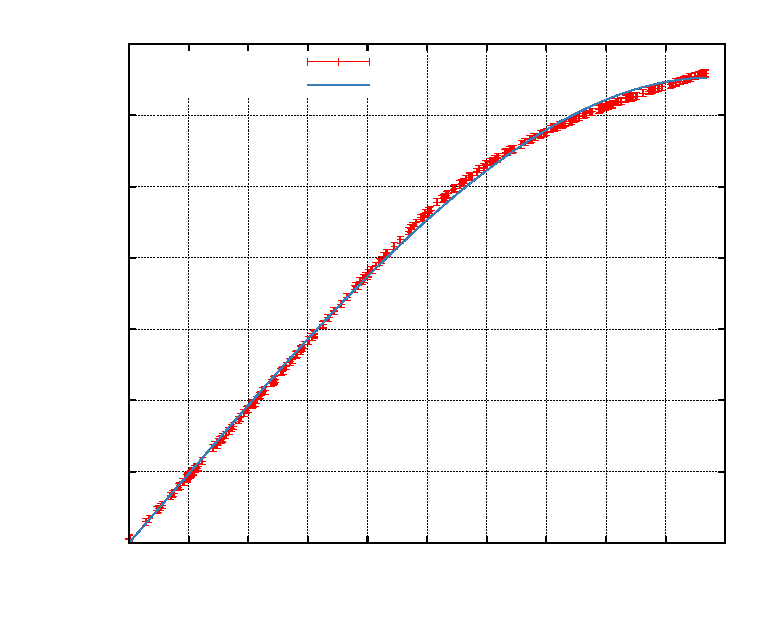
\includegraphics{./plots/kalibrierung1}}%
    \gplfronttext
  \end{picture}%
\endgroup

\caption{Erster Durchgang kalibrierung}
\label{fig:kalibrierung1}
\end{figure}

\begin{figure}[h]
\centering
% GNUPLOT: LaTeX picture with Postscript
\begingroup
  \makeatletter
  \providecommand\color[2][]{%
    \GenericError{(gnuplot) \space\space\space\@spaces}{%
      Package color not loaded in conjunction with
      terminal option `colourtext'%
    }{See the gnuplot documentation for explanation.%
    }{Either use 'blacktext' in gnuplot or load the package
      color.sty in LaTeX.}%
    \renewcommand\color[2][]{}%
  }%
  \providecommand\includegraphics[2][]{%
    \GenericError{(gnuplot) \space\space\space\@spaces}{%
      Package graphicx or graphics not loaded%
    }{See the gnuplot documentation for explanation.%
    }{The gnuplot epslatex terminal needs graphicx.sty or graphics.sty.}%
    \renewcommand\includegraphics[2][]{}%
  }%
  \providecommand\rotatebox[2]{#2}%
  \@ifundefined{ifGPcolor}{%
    \newif\ifGPcolor
    \GPcolortrue
  }{}%
  \@ifundefined{ifGPblacktext}{%
    \newif\ifGPblacktext
    \GPblacktexttrue
  }{}%
  % define a \g@addto@macro without @ in the name:
  \let\gplgaddtomacro\g@addto@macro
  % define empty templates for all commands taking text:
  \gdef\gplbacktext{}%
  \gdef\gplfronttext{}%
  \makeatother
  \ifGPblacktext
    % no textcolor at all
    \def\colorrgb#1{}%
    \def\colorgray#1{}%
  \else
    % gray or color?
    \ifGPcolor
      \def\colorrgb#1{\color[rgb]{#1}}%
      \def\colorgray#1{\color[gray]{#1}}%
      \expandafter\def\csname LTw\endcsname{\color{white}}%
      \expandafter\def\csname LTb\endcsname{\color{black}}%
      \expandafter\def\csname LTa\endcsname{\color{black}}%
      \expandafter\def\csname LT0\endcsname{\color[rgb]{1,0,0}}%
      \expandafter\def\csname LT1\endcsname{\color[rgb]{0,1,0}}%
      \expandafter\def\csname LT2\endcsname{\color[rgb]{0,0,1}}%
      \expandafter\def\csname LT3\endcsname{\color[rgb]{1,0,1}}%
      \expandafter\def\csname LT4\endcsname{\color[rgb]{0,1,1}}%
      \expandafter\def\csname LT5\endcsname{\color[rgb]{1,1,0}}%
      \expandafter\def\csname LT6\endcsname{\color[rgb]{0,0,0}}%
      \expandafter\def\csname LT7\endcsname{\color[rgb]{1,0.3,0}}%
      \expandafter\def\csname LT8\endcsname{\color[rgb]{0.5,0.5,0.5}}%
    \else
      % gray
      \def\colorrgb#1{\color{black}}%
      \def\colorgray#1{\color[gray]{#1}}%
      \expandafter\def\csname LTw\endcsname{\color{white}}%
      \expandafter\def\csname LTb\endcsname{\color{black}}%
      \expandafter\def\csname LTa\endcsname{\color{black}}%
      \expandafter\def\csname LT0\endcsname{\color{black}}%
      \expandafter\def\csname LT1\endcsname{\color{black}}%
      \expandafter\def\csname LT2\endcsname{\color{black}}%
      \expandafter\def\csname LT3\endcsname{\color{black}}%
      \expandafter\def\csname LT4\endcsname{\color{black}}%
      \expandafter\def\csname LT5\endcsname{\color{black}}%
      \expandafter\def\csname LT6\endcsname{\color{black}}%
      \expandafter\def\csname LT7\endcsname{\color{black}}%
      \expandafter\def\csname LT8\endcsname{\color{black}}%
    \fi
  \fi
  \setlength{\unitlength}{0.0500bp}%
  \begin{picture}(7200.00,5760.00)%
    \gplgaddtomacro\gplbacktext{%
      \csname LTb\endcsname%
      \put(946,704){\makebox(0,0)[r]{\strut{} 0}}%
      \csname LTb\endcsname%
      \put(946,1388){\makebox(0,0)[r]{\strut{} 100}}%
      \csname LTb\endcsname%
      \put(946,2073){\makebox(0,0)[r]{\strut{} 200}}%
      \csname LTb\endcsname%
      \put(946,2757){\makebox(0,0)[r]{\strut{} 300}}%
      \csname LTb\endcsname%
      \put(946,3442){\makebox(0,0)[r]{\strut{} 400}}%
      \csname LTb\endcsname%
      \put(946,4126){\makebox(0,0)[r]{\strut{} 500}}%
      \csname LTb\endcsname%
      \put(946,4811){\makebox(0,0)[r]{\strut{} 600}}%
      \csname LTb\endcsname%
      \put(946,5495){\makebox(0,0)[r]{\strut{} 700}}%
      \csname LTb\endcsname%
      \put(1078,484){\makebox(0,0){\strut{} 0}}%
      \csname LTb\endcsname%
      \put(1651,484){\makebox(0,0){\strut{} 1}}%
      \csname LTb\endcsname%
      \put(2223,484){\makebox(0,0){\strut{} 2}}%
      \csname LTb\endcsname%
      \put(2796,484){\makebox(0,0){\strut{} 3}}%
      \csname LTb\endcsname%
      \put(3368,484){\makebox(0,0){\strut{} 4}}%
      \csname LTb\endcsname%
      \put(3941,484){\makebox(0,0){\strut{} 5}}%
      \csname LTb\endcsname%
      \put(4513,484){\makebox(0,0){\strut{} 6}}%
      \csname LTb\endcsname%
      \put(5086,484){\makebox(0,0){\strut{} 7}}%
      \csname LTb\endcsname%
      \put(5658,484){\makebox(0,0){\strut{} 8}}%
      \csname LTb\endcsname%
      \put(6231,484){\makebox(0,0){\strut{} 9}}%
      \csname LTb\endcsname%
      \put(6803,484){\makebox(0,0){\strut{} 10}}%
      \put(176,3099){\rotatebox{-270}{\makebox(0,0){\strut{}Magnetfeld $B$ im Luftspalt / \si{\milli\tesla}}}}%
      \put(3940,154){\makebox(0,0){\strut{}Spulenstrom $I$ / \si{\ampere}}}%
      \put(3940,5385){\makebox(0,0){\strut{}}}%
    }%
    \gplgaddtomacro\gplfronttext{%
      \csname LTb\endcsname%
      \put(2662,5322){\makebox(0,0)[r]{\strut{}Messwerte}}%
      \csname LTb\endcsname%
      \put(2662,5102){\makebox(0,0)[r]{\strut{}Fitfunktion}}%
    }%
    \gplbacktext
    \put(0,0){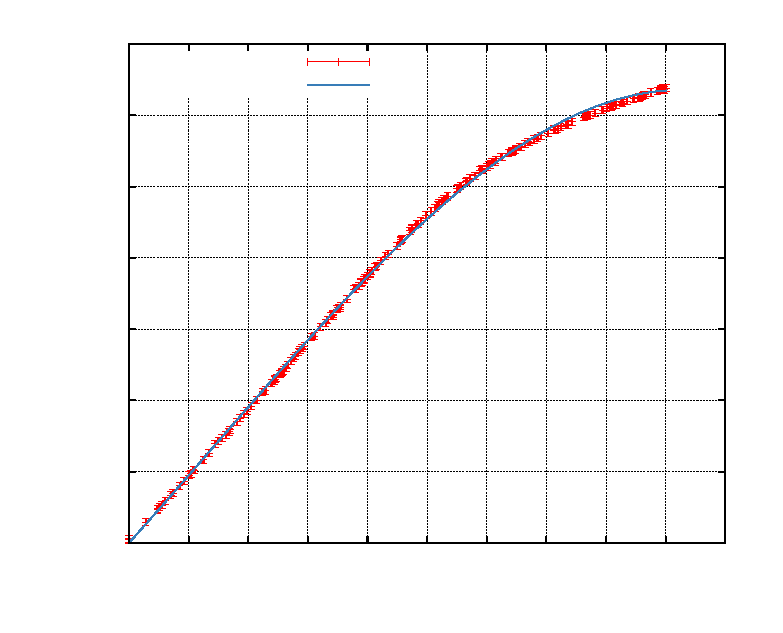
\includegraphics{./plots/kalibrierung2}}%
    \gplfronttext
  \end{picture}%
\endgroup

\caption{Zweiter Durchgang kalibrierung}
\label{fig:kalibrierung2}
\end{figure}



\FloatBarrier
\subsection{Auswertung}
Auswahl des untersuchten Peaks hier!

Gaußfunktion:
\begin{align}
	\mathcal{G}_i(x) = A_i \exp\left( -\frac{1}{2} \left( \frac{x - \mu_i}{\sigma_i} \right)^2 \right)
\end{align}

Fithypothese:
\begin{align}
	f(x) = \mathcal{G}_1(x) + \mathcal{G}_2(x) + \mathcal{G}_3(x) + d
\end{align}

$\mathcal{G}_1$ entspricht der $\sigma_-$-Linie, $\mathcal{G}_2$ entspricht $\pi$-Linie, $\mathcal{G}_3$ entspricht $\sigma_+$-Linie.

Mit den Fits an die Messdaten erhalten wir Tabelle \ref{tab:peakschwerpunkte_magneton}.

\begin{table}[h]
	\centering
	\resizebox{\columnwidth}{!}{%
		\begin{tabular}{SSSSSSS}
\toprule
{Strom $I$ / \si{\ampere}} & {$\alpha_-$ / \si{\milli\degree}}& {$\sigma_{\alpha_-}$ / \si{\milli\degree}}& {$\alpha_0$ / \si{\milli\degree}} &{$\sigma_{\alpha_0}$ / \si{\milli\degree}} & {$\alpha_+$ / \si{\milli\degree}} & {$\sigma_{\alpha_+}$ / \si{\milli\degree}}\\
\midrule
4.0	&	938.25&	0.59	&		1015.47&	0.31	&		1084.82&	0.62	\\
4.5	&	926.15&	0.35	&		1013.00&	0.23	&		1091.78&	0.48	\\
5.0	&	915.79&	0.45	&		1011.60&	0.31	&		1098.57&	0.58	\\
5.5	&	907.63&	0.43	&		1010.37&	0.31	&		1103.19&	0.56	\\
6.0	&	899.42&	0.56	&		1009.48&	0.38	&		1108.59&	0.73	\\
6.5	&	892.78&	0.64	&		1008.75&	0.43	&		1113.06&	0.84	\\
7.0	&	887.92&	0.72	&		1007.77&	0.48	&		1115.89&	1.00	\\
7.5	&	883.05&	0.83	&		1007.17&	0.55	&		1119.34&	1.24	\\
8.0	&	879.59&	0.83	&		1006.73&	0.48	&		1120.66&	1.13	\\
8.5	&	874.79&	0.75	&		1005.64&	0.47	&		1122.76&	1.13	\\
8.9	&	871.95&	0.75	&		1005.28&	0.39	&		1123.36&	0.96	\\
\bottomrule
\end{tabular}}
	\caption{Gefittete Werte für die Schwerpunkte $\alpha_i$ der drei Linien. Angaben in Milligrad.}
	\label{tab:peakschwerpunkte_magneton}
\end{table}

Berechnung der relativen Abweichung von der $\pi$-Linie mit der Interferenzbedingung \ref{eq:interferenzbedingung}:
\begin{align}
	\frac{\Delta \lambda_\pm}{\lambda_\pi^0} = \frac{\lambda_{\sigma^\pm} - \lambda_\pi^0}{\lambda_\pi^0} = \frac{\sqrt{n^2 - \sin^2(\alpha_{\pm})}}{\sqrt{n^2 - \sin^2(\alpha_0)}} - 1
\end{align}

Der Fehler berechnet sich mit Gaußscher Fehlerfortpflanzung zu:
\begin{align}
	\Delta \left( \frac{\Delta \lambda_\pm}{\lambda_\pi^0} \right) = & \left( \frac{\sin^2(\alpha_\pm) \cos^2(\alpha_\pm)}{(n^2-\sin^2(\alpha_\pm))(n^2-\sin^2(\alpha_0))} \cdot \Delta \alpha_\pm^2 \right. \nonumber\\
	& \left. + \frac{\sin^2(\alpha_0) \cos^2(\alpha_0) (n^2 - \sin^2(\alpha_\pm))}{(n^2-\sin^2(\alpha_0))^3} \cdot \Delta \alpha_0^2\right)^\frac{1}{2}
\end{align}

\begin{table}[h]
	\centering
	\begin{tabular}{SSSSS}
\toprule
{$I$ / \si{\ampere}} & {$\frac{\Delta \lambda_{-}}{\lambda_\pi^0}$} & {$\sigma_\mathrm{rel.}^{-}$} & {$\frac{\Delta \lambda_{+}}{\lambda_\pi^0}$} & {$\sigma_\mathrm{rel.}^{+}$} \\
\midrule
4.0 & 1.0824 & 0.0090 & -1.0450 & 0.0107 \\
4.5 & 1.2083 & 0.0058 & -1.1896 & 0.0080 \\
5.0 & 1.3249 & 0.0074 & -1.3166 & 0.0102 \\
5.5 & 1.4138 & 0.0071 & -1.4074 & 0.0099 \\
6.0 & 1.5072 & 0.0091 & -1.5060 & 0.0128 \\
6.5 & 1.5822 & 0.0102 & -1.5878 & 0.0147 \\
7.0 & 1.6300 & 0.0139 & -1.6473 & 0.0174 \\
7.5 & 1.6832 & 0.0132 & -1.7113 & 0.0215 \\
8.0 & 1.7206 & 0.0125 & -1.7388 & 0.0194 \\
8.5 & 1.7654 & 0.0116 & -1.7884 & 0.0193 \\
8.9 & 1.7957 & 0.0109 & -1.8032 & 0.0164 \\
\bottomrule
\end{tabular}
	\caption{Wellenlängenverschiebung}
	\label{tab:verschiebung_wellenlaenge}
\end{table}

Nun schätzen wir die Beugungsordnung durch:
\begin{align}
	m \approx \frac{2 d}{\lambda} = 18104
\end{align}


\begin{figure}[h]
	\centering
	% GNUPLOT: LaTeX picture with Postscript
\begingroup
  \makeatletter
  \providecommand\color[2][]{%
    \GenericError{(gnuplot) \space\space\space\@spaces}{%
      Package color not loaded in conjunction with
      terminal option `colourtext'%
    }{See the gnuplot documentation for explanation.%
    }{Either use 'blacktext' in gnuplot or load the package
      color.sty in LaTeX.}%
    \renewcommand\color[2][]{}%
  }%
  \providecommand\includegraphics[2][]{%
    \GenericError{(gnuplot) \space\space\space\@spaces}{%
      Package graphicx or graphics not loaded%
    }{See the gnuplot documentation for explanation.%
    }{The gnuplot epslatex terminal needs graphicx.sty or graphics.sty.}%
    \renewcommand\includegraphics[2][]{}%
  }%
  \providecommand\rotatebox[2]{#2}%
  \@ifundefined{ifGPcolor}{%
    \newif\ifGPcolor
    \GPcolortrue
  }{}%
  \@ifundefined{ifGPblacktext}{%
    \newif\ifGPblacktext
    \GPblacktexttrue
  }{}%
  % define a \g@addto@macro without @ in the name:
  \let\gplgaddtomacro\g@addto@macro
  % define empty templates for all commands taking text:
  \gdef\gplbacktext{}%
  \gdef\gplfronttext{}%
  \makeatother
  \ifGPblacktext
    % no textcolor at all
    \def\colorrgb#1{}%
    \def\colorgray#1{}%
  \else
    % gray or color?
    \ifGPcolor
      \def\colorrgb#1{\color[rgb]{#1}}%
      \def\colorgray#1{\color[gray]{#1}}%
      \expandafter\def\csname LTw\endcsname{\color{white}}%
      \expandafter\def\csname LTb\endcsname{\color{black}}%
      \expandafter\def\csname LTa\endcsname{\color{black}}%
      \expandafter\def\csname LT0\endcsname{\color[rgb]{1,0,0}}%
      \expandafter\def\csname LT1\endcsname{\color[rgb]{0,1,0}}%
      \expandafter\def\csname LT2\endcsname{\color[rgb]{0,0,1}}%
      \expandafter\def\csname LT3\endcsname{\color[rgb]{1,0,1}}%
      \expandafter\def\csname LT4\endcsname{\color[rgb]{0,1,1}}%
      \expandafter\def\csname LT5\endcsname{\color[rgb]{1,1,0}}%
      \expandafter\def\csname LT6\endcsname{\color[rgb]{0,0,0}}%
      \expandafter\def\csname LT7\endcsname{\color[rgb]{1,0.3,0}}%
      \expandafter\def\csname LT8\endcsname{\color[rgb]{0.5,0.5,0.5}}%
    \else
      % gray
      \def\colorrgb#1{\color{black}}%
      \def\colorgray#1{\color[gray]{#1}}%
      \expandafter\def\csname LTw\endcsname{\color{white}}%
      \expandafter\def\csname LTb\endcsname{\color{black}}%
      \expandafter\def\csname LTa\endcsname{\color{black}}%
      \expandafter\def\csname LT0\endcsname{\color{black}}%
      \expandafter\def\csname LT1\endcsname{\color{black}}%
      \expandafter\def\csname LT2\endcsname{\color{black}}%
      \expandafter\def\csname LT3\endcsname{\color{black}}%
      \expandafter\def\csname LT4\endcsname{\color{black}}%
      \expandafter\def\csname LT5\endcsname{\color{black}}%
      \expandafter\def\csname LT6\endcsname{\color{black}}%
      \expandafter\def\csname LT7\endcsname{\color{black}}%
      \expandafter\def\csname LT8\endcsname{\color{black}}%
    \fi
  \fi
  \setlength{\unitlength}{0.0500bp}%
  \begin{picture}(7488.00,5040.00)%
    \gplgaddtomacro\gplbacktext{%
      \csname LTb\endcsname%
      \put(946,704){\makebox(0,0)[r]{\strut{} 0}}%
      \csname LTb\endcsname%
      \put(946,1156){\makebox(0,0)[r]{\strut{} 0.5}}%
      \csname LTb\endcsname%
      \put(946,1609){\makebox(0,0)[r]{\strut{} 1}}%
      \csname LTb\endcsname%
      \put(946,2061){\makebox(0,0)[r]{\strut{} 1.5}}%
      \csname LTb\endcsname%
      \put(946,2513){\makebox(0,0)[r]{\strut{} 2}}%
      \csname LTb\endcsname%
      \put(946,2966){\makebox(0,0)[r]{\strut{} 2.5}}%
      \csname LTb\endcsname%
      \put(946,3418){\makebox(0,0)[r]{\strut{} 3}}%
      \csname LTb\endcsname%
      \put(946,3870){\makebox(0,0)[r]{\strut{} 3.5}}%
      \csname LTb\endcsname%
      \put(946,4323){\makebox(0,0)[r]{\strut{} 4}}%
      \csname LTb\endcsname%
      \put(946,4775){\makebox(0,0)[r]{\strut{} 4.5}}%
      \csname LTb\endcsname%
      \put(1078,484){\makebox(0,0){\strut{} 350}}%
      \csname LTb\endcsname%
      \put(1937,484){\makebox(0,0){\strut{} 400}}%
      \csname LTb\endcsname%
      \put(2796,484){\makebox(0,0){\strut{} 450}}%
      \csname LTb\endcsname%
      \put(3655,484){\makebox(0,0){\strut{} 500}}%
      \csname LTb\endcsname%
      \put(4514,484){\makebox(0,0){\strut{} 550}}%
      \csname LTb\endcsname%
      \put(5373,484){\makebox(0,0){\strut{} 600}}%
      \csname LTb\endcsname%
      \put(6232,484){\makebox(0,0){\strut{} 650}}%
      \csname LTb\endcsname%
      \put(7091,484){\makebox(0,0){\strut{} 700}}%
      \put(176,2739){\rotatebox{-270}{\makebox(0,0){\strut{}E / $10^{-5} \si{\electronvolt}$}}}%
      \put(4084,154){\makebox(0,0){\strut{}B / $\si{\milli\tesla}$}}%
      \put(4084,4665){\makebox(0,0){\strut{}}}%
    }%
    \gplgaddtomacro\gplfronttext{%
      \csname LTb\endcsname%
      \put(2398,4602){\makebox(0,0)[r]{\strut{}E-}}%
      \csname LTb\endcsname%
      \put(2398,4382){\makebox(0,0)[r]{\strut{}E+}}%
      \csname LTb\endcsname%
      \put(2398,4162){\makebox(0,0)[r]{\strut{}E-}}%
      \csname LTb\endcsname%
      \put(2398,3942){\makebox(0,0)[r]{\strut{}E+}}%
      \csname LTb\endcsname%
      \put(2398,3722){\makebox(0,0)[r]{\strut{}Literatur}}%
    }%
    \gplbacktext
    \put(0,0){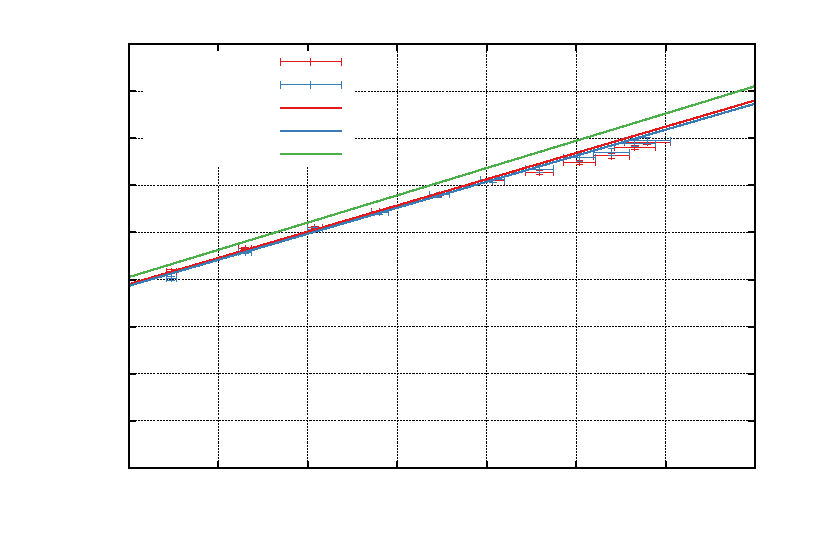
\includegraphics{./plots/magneton_fit}}%
    \gplfronttext
  \end{picture}%
\endgroup

	\caption{magneton fit}
	\label{fig:magneton_fit}
\end{figure}


\begin{figure}[h]
	\centering
	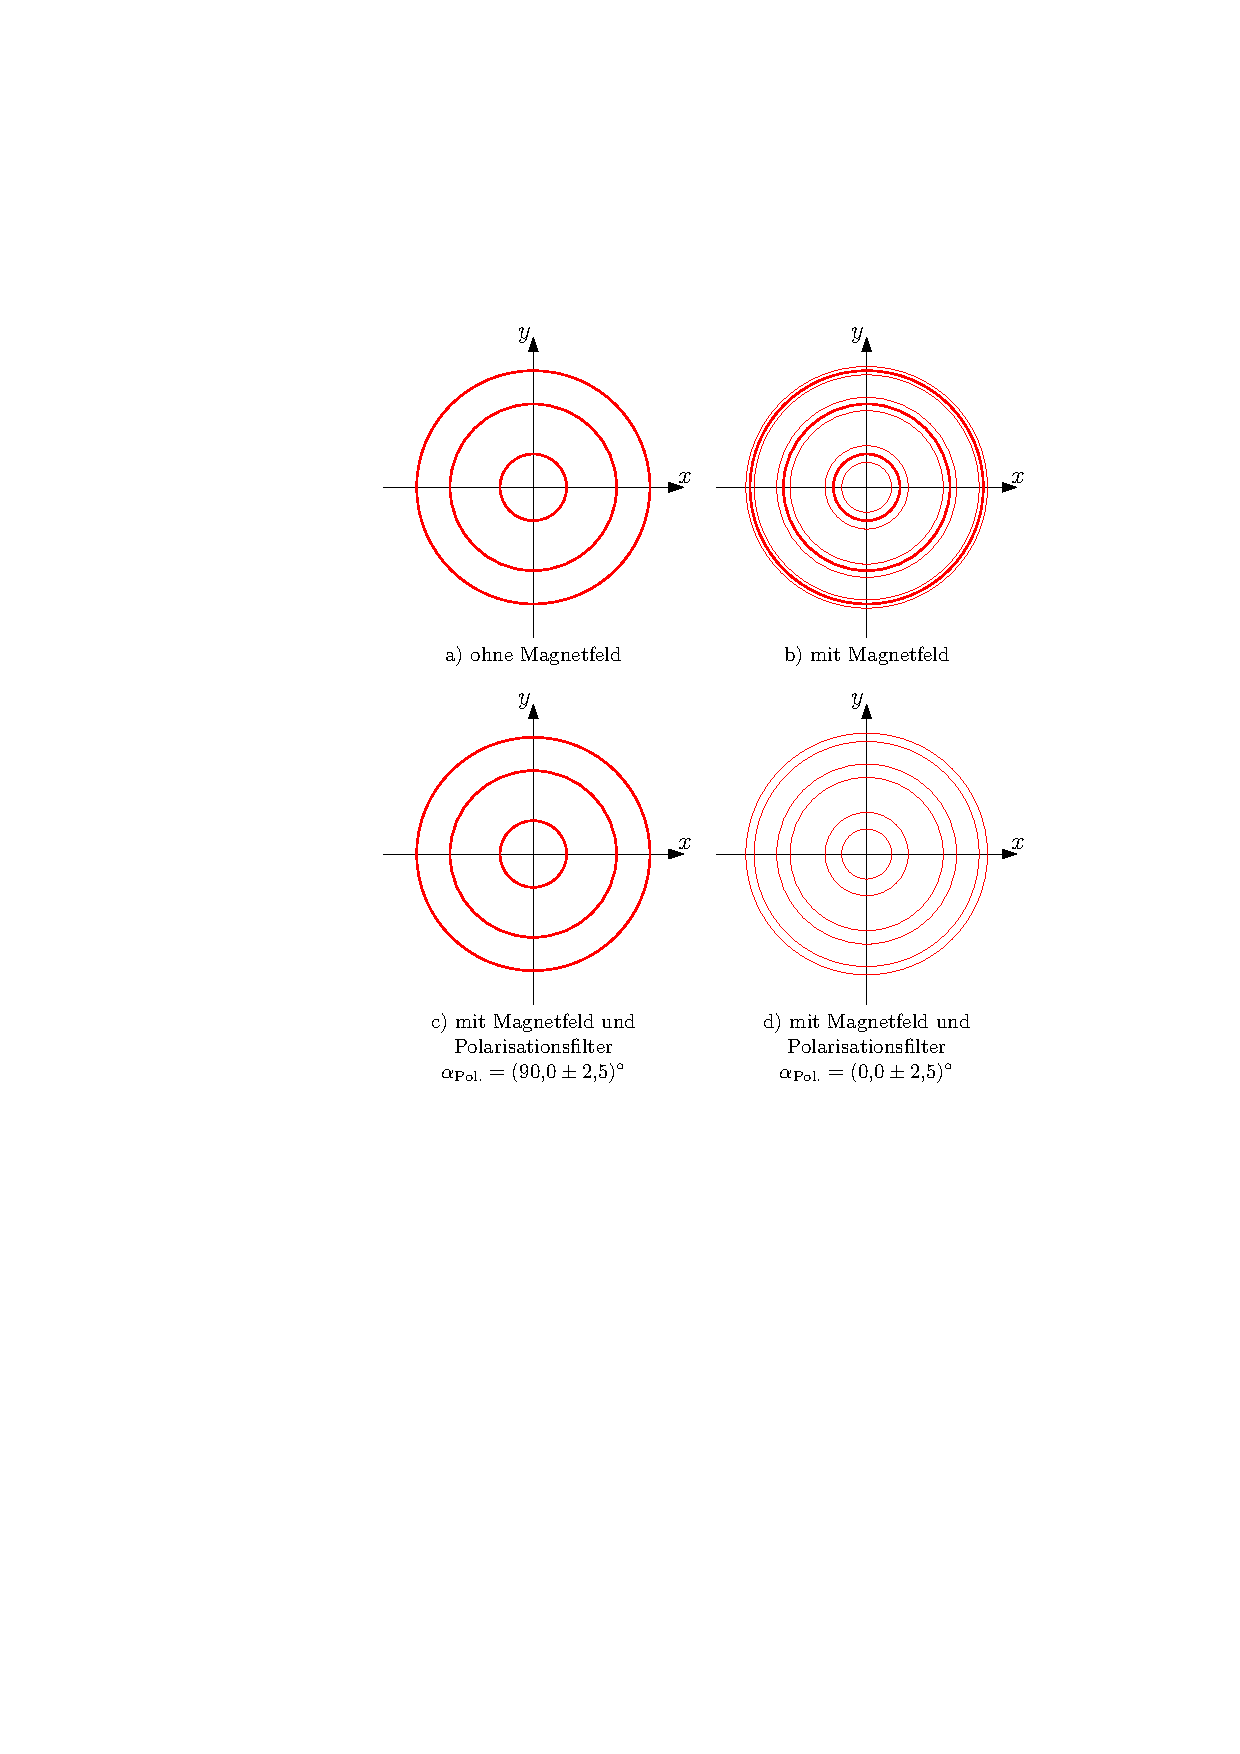
\includegraphics[width=0.9\textwidth]{./figures/zeeman_transversal.pdf}
	\caption{transversal}
	\label{fig:zeeman_transversal}
\end{figure}

\begin{figure}[h]
	\centering
	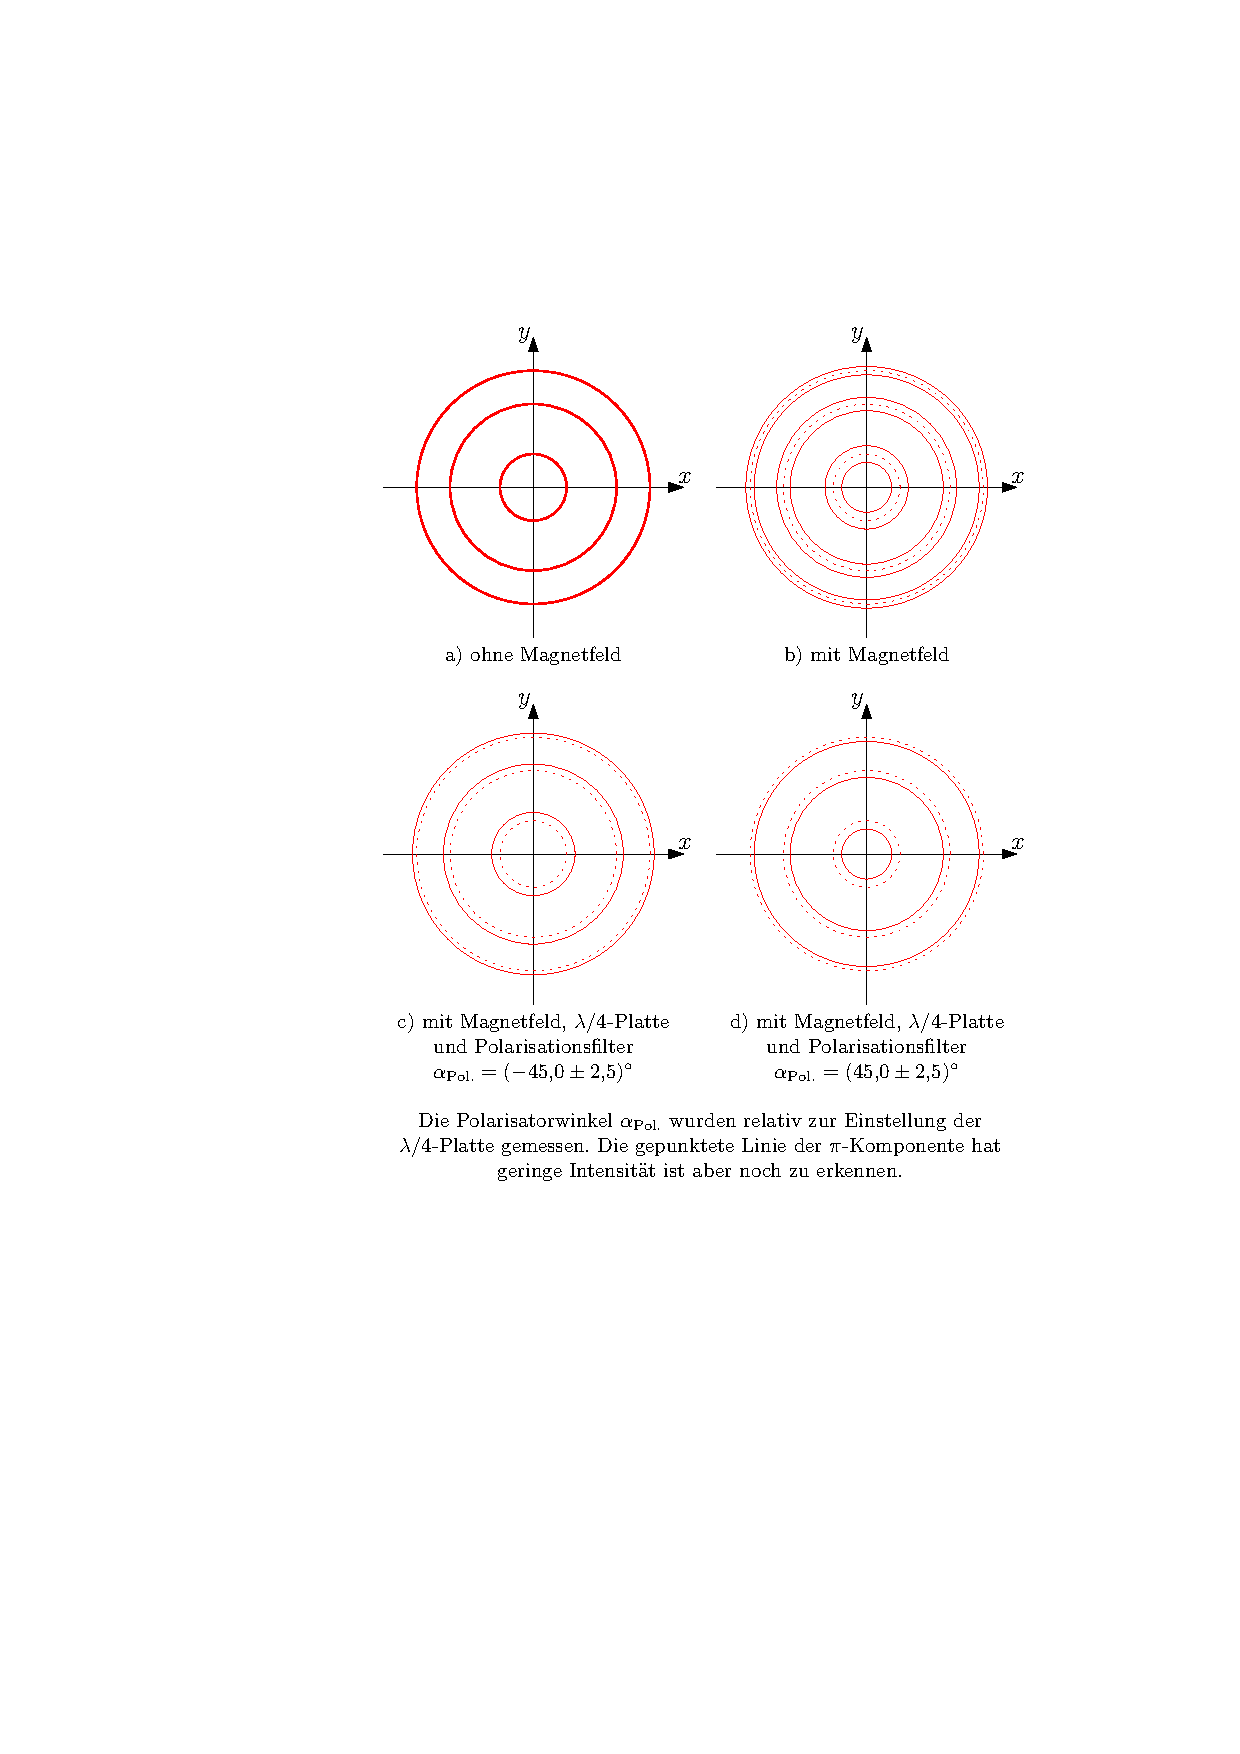
\includegraphics[width=0.9\textwidth]{./figures/zeeman_longitudinal.pdf}
	\caption{longitudinal}
	\label{fig:zeeman_longitudinal}
\end{figure}

\begin{table}[h]
	\centering
	\begin{tabular}{lS}
\toprule
{\#} & {$I / \si{\ampere}$} \\
\midrule
1&	2.1 +- 0.1 \\
2&	2.1 +- 0.1 \\
3&	2.0 +- 0.1 \\
4&	2.0 +- 0.1 \\
5&	2.0 +- 0.1 \\
\bottomrule
\end{tabular}
	\caption{Messdaten zur Bestimmung der Auflösung in transversalem Aufbau}
	\label{tab:aufloesung_transversal}
\end{table}

\begin{table}[h]
	\centering
	\begin{tabular}{lS}
\toprule
{\#} & {$I / \si{\ampere}$} \\
\midrule
1&	1.7 +- 0.1 \\
2&	1.6 +- 0.1 \\
3&	1.6 +- 0.1 \\
4&	1.5 +- 0.1 \\
5&	1.6 +- 0.1 \\
\bottomrule
\end{tabular}
	\caption{Messdaten zur Bestimmung der Auflösung in longitudinalem Aufbau}
	\label{tab:aufloesung_longitudinal}
\end{table}

\subsection{Diskussion}

% damit ich nicht wahnsinnig werde
\FloatBarrier

\section{Franck-Hertz-Versuch}
Hier kurze Einführung (was wird gemacht)

\subsection{Durchführung}

Der Versuch war bereits fertig aufgebaut, so dass lediglich das Cassy-Instrument in Betrieb genommen werden musste.
Dieses misst einmal die vom Steuergerät der Röhre ausgegebene Beschleunigungsspannung und digitalisiert die am anderen Ausgang liegende Spannung, die intern über einen Widerstand aus dem Anodenstrom gewonnen wird.
Da $U=R\,I$ gilt und konkrete Werte des Anodenstroms für die Auswertung irrelevant sind, braucht diese Umwandlung nicht weiter berücksichtigt werden.

An dem Gerät, das mit dem Ofen verbunden ist, können diverse Parameter eingestellt werden, unter anderem die für uns relevante Signalform der Beschleunigungsspannung (wir wählen gemäß der Anleitung eine positive Rampe), sowie deren Maximalwert.
Weiterhin können Temperatur der Röhre eingestellt und aktuelle Temperaturwerte überprüft werden, sowie einige weitere Optionen, die für den Versuch nicht benötigt wurden.

Vor jeder Messung haben wir mit der Option, manuell die Beschleunigungsspannung einzustellen, diese langsam erhöht bis der Effekt des Durchzündens erkennbar war und haben dann für den Maximalwert der Beschleunigungsspannung einen leicht darunter liegenden Wert gewählt, um den Aufbau nicht zu beschädigen.

\subsection{Messdaten}

Zunächst führen wir die Messung für verschiedene Gegenspannungen bei konstanter Temperatur durch.
Für diese wählen wir \SI{160}{\degreeCelsius} und überprüfen vor den Messungen, wie oben angesprochen, dass kein Durchzünden stattfinden kann.
Darum wählen wir als Maximalwert der positiven Rampe \SI{42}{\kilo\volt} und messen für vier Gegenspannungen zwischen \SI{2}{\volt} und \SI{3.5}{\volt} den Anodenstrom.
Die Messwerte sind in Abbildung \ref{fig:fh_varvolt} dargestellt.
Für die Diagramme wählen wir zur Skalierung der y-Achse willkürliche Einheiten, da diese nicht zur Auswertung benötigt werden und durch die im Steuergerät durchgeführte Umwandlung des Stroms in eine von Cassy messbare Spannung der Umrechnungsfaktor nicht bekannt ist.
\begin{figure}[!h]
\centering
% GNUPLOT: LaTeX picture with Postscript
\begingroup
  \makeatletter
  \providecommand\color[2][]{%
    \GenericError{(gnuplot) \space\space\space\@spaces}{%
      Package color not loaded in conjunction with
      terminal option `colourtext'%
    }{See the gnuplot documentation for explanation.%
    }{Either use 'blacktext' in gnuplot or load the package
      color.sty in LaTeX.}%
    \renewcommand\color[2][]{}%
  }%
  \providecommand\includegraphics[2][]{%
    \GenericError{(gnuplot) \space\space\space\@spaces}{%
      Package graphicx or graphics not loaded%
    }{See the gnuplot documentation for explanation.%
    }{The gnuplot epslatex terminal needs graphicx.sty or graphics.sty.}%
    \renewcommand\includegraphics[2][]{}%
  }%
  \providecommand\rotatebox[2]{#2}%
  \@ifundefined{ifGPcolor}{%
    \newif\ifGPcolor
    \GPcolortrue
  }{}%
  \@ifundefined{ifGPblacktext}{%
    \newif\ifGPblacktext
    \GPblacktexttrue
  }{}%
  % define a \g@addto@macro without @ in the name:
  \let\gplgaddtomacro\g@addto@macro
  % define empty templates for all commands taking text:
  \gdef\gplbacktext{}%
  \gdef\gplfronttext{}%
  \makeatother
  \ifGPblacktext
    % no textcolor at all
    \def\colorrgb#1{}%
    \def\colorgray#1{}%
  \else
    % gray or color?
    \ifGPcolor
      \def\colorrgb#1{\color[rgb]{#1}}%
      \def\colorgray#1{\color[gray]{#1}}%
      \expandafter\def\csname LTw\endcsname{\color{white}}%
      \expandafter\def\csname LTb\endcsname{\color{black}}%
      \expandafter\def\csname LTa\endcsname{\color{black}}%
      \expandafter\def\csname LT0\endcsname{\color[rgb]{1,0,0}}%
      \expandafter\def\csname LT1\endcsname{\color[rgb]{0,1,0}}%
      \expandafter\def\csname LT2\endcsname{\color[rgb]{0,0,1}}%
      \expandafter\def\csname LT3\endcsname{\color[rgb]{1,0,1}}%
      \expandafter\def\csname LT4\endcsname{\color[rgb]{0,1,1}}%
      \expandafter\def\csname LT5\endcsname{\color[rgb]{1,1,0}}%
      \expandafter\def\csname LT6\endcsname{\color[rgb]{0,0,0}}%
      \expandafter\def\csname LT7\endcsname{\color[rgb]{1,0.3,0}}%
      \expandafter\def\csname LT8\endcsname{\color[rgb]{0.5,0.5,0.5}}%
    \else
      % gray
      \def\colorrgb#1{\color{black}}%
      \def\colorgray#1{\color[gray]{#1}}%
      \expandafter\def\csname LTw\endcsname{\color{white}}%
      \expandafter\def\csname LTb\endcsname{\color{black}}%
      \expandafter\def\csname LTa\endcsname{\color{black}}%
      \expandafter\def\csname LT0\endcsname{\color{black}}%
      \expandafter\def\csname LT1\endcsname{\color{black}}%
      \expandafter\def\csname LT2\endcsname{\color{black}}%
      \expandafter\def\csname LT3\endcsname{\color{black}}%
      \expandafter\def\csname LT4\endcsname{\color{black}}%
      \expandafter\def\csname LT5\endcsname{\color{black}}%
      \expandafter\def\csname LT6\endcsname{\color{black}}%
      \expandafter\def\csname LT7\endcsname{\color{black}}%
      \expandafter\def\csname LT8\endcsname{\color{black}}%
    \fi
  \fi
  \setlength{\unitlength}{0.0500bp}%
  \begin{picture}(7200.00,5760.00)%
    \gplgaddtomacro\gplbacktext{%
      \csname LTb\endcsname%
      \put(814,704){\makebox(0,0)[r]{\strut{} 0}}%
      \csname LTb\endcsname%
      \put(814,1662){\makebox(0,0)[r]{\strut{} 2}}%
      \csname LTb\endcsname%
      \put(814,2620){\makebox(0,0)[r]{\strut{} 4}}%
      \csname LTb\endcsname%
      \put(814,3579){\makebox(0,0)[r]{\strut{} 6}}%
      \csname LTb\endcsname%
      \put(814,4537){\makebox(0,0)[r]{\strut{} 8}}%
      \csname LTb\endcsname%
      \put(814,5495){\makebox(0,0)[r]{\strut{} 10}}%
      \csname LTb\endcsname%
      \put(946,484){\makebox(0,0){\strut{} 0}}%
      \csname LTb\endcsname%
      \put(1678,484){\makebox(0,0){\strut{} 5}}%
      \csname LTb\endcsname%
      \put(2410,484){\makebox(0,0){\strut{} 10}}%
      \csname LTb\endcsname%
      \put(3142,484){\makebox(0,0){\strut{} 15}}%
      \csname LTb\endcsname%
      \put(3875,484){\makebox(0,0){\strut{} 20}}%
      \csname LTb\endcsname%
      \put(4607,484){\makebox(0,0){\strut{} 25}}%
      \csname LTb\endcsname%
      \put(5339,484){\makebox(0,0){\strut{} 30}}%
      \csname LTb\endcsname%
      \put(6071,484){\makebox(0,0){\strut{} 35}}%
      \csname LTb\endcsname%
      \put(6803,484){\makebox(0,0){\strut{} 40}}%
      \put(176,3099){\rotatebox{-270}{\makebox(0,0){\strut{}Anodenstrom $I$ / w.E.}}}%
      \put(3874,154){\makebox(0,0){\strut{}Beschleunigungsspannung $U$ / \si{\kilo\volt}}}%
      \put(3874,5385){\makebox(0,0){\strut{}}}%
    }%
    \gplgaddtomacro\gplfronttext{%
      \csname LTb\endcsname%
      \put(2266,5322){\makebox(0,0)[r]{\strut{}$\Delta U=\SI{2.0}{\volt}$}}%
      \csname LTb\endcsname%
      \put(2266,5102){\makebox(0,0)[r]{\strut{}$\Delta U=\SI{2.5}{\volt}$}}%
      \csname LTb\endcsname%
      \put(2266,4882){\makebox(0,0)[r]{\strut{}$\Delta U=\SI{3.0}{\volt}$}}%
      \csname LTb\endcsname%
      \put(2266,4662){\makebox(0,0)[r]{\strut{}$\Delta U=\SI{3.5}{\volt}$}}%
    }%
    \gplbacktext
    \put(0,0){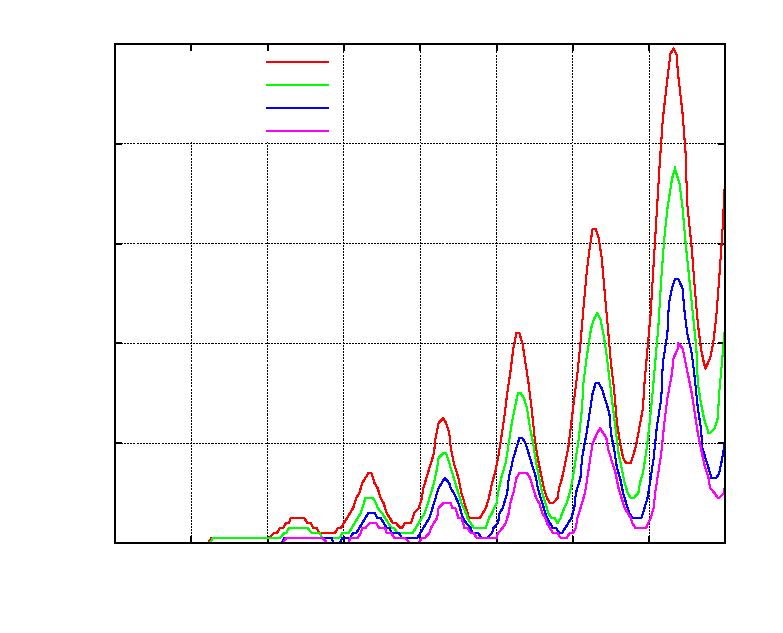
\includegraphics{./plots/fh_varvolt}}%
    \gplfronttext
  \end{picture}%
\endgroup

\caption{Variable Gegenspannung bei $T=\SI{160}{\degreeCelsius}$}
\label{fig:fh_varvolt}
\end{figure}
Für die Messung mit variabler Temperatur erhalten wir die in Abbildung \ref{fig:fh_vartemp} dargestellten Ergebnisse.
Dabei wählten wir als konstante Gegenspannung \SI{2}{\volt} und nutzen wieder willkürliche Einheiten für den gemessenen Anodenstrom.
\begin{figure}[!h]
\centering
% GNUPLOT: LaTeX picture with Postscript
\begingroup
  \makeatletter
  \providecommand\color[2][]{%
    \GenericError{(gnuplot) \space\space\space\@spaces}{%
      Package color not loaded in conjunction with
      terminal option `colourtext'%
    }{See the gnuplot documentation for explanation.%
    }{Either use 'blacktext' in gnuplot or load the package
      color.sty in LaTeX.}%
    \renewcommand\color[2][]{}%
  }%
  \providecommand\includegraphics[2][]{%
    \GenericError{(gnuplot) \space\space\space\@spaces}{%
      Package graphicx or graphics not loaded%
    }{See the gnuplot documentation for explanation.%
    }{The gnuplot epslatex terminal needs graphicx.sty or graphics.sty.}%
    \renewcommand\includegraphics[2][]{}%
  }%
  \providecommand\rotatebox[2]{#2}%
  \@ifundefined{ifGPcolor}{%
    \newif\ifGPcolor
    \GPcolortrue
  }{}%
  \@ifundefined{ifGPblacktext}{%
    \newif\ifGPblacktext
    \GPblacktexttrue
  }{}%
  % define a \g@addto@macro without @ in the name:
  \let\gplgaddtomacro\g@addto@macro
  % define empty templates for all commands taking text:
  \gdef\gplbacktext{}%
  \gdef\gplfronttext{}%
  \makeatother
  \ifGPblacktext
    % no textcolor at all
    \def\colorrgb#1{}%
    \def\colorgray#1{}%
  \else
    % gray or color?
    \ifGPcolor
      \def\colorrgb#1{\color[rgb]{#1}}%
      \def\colorgray#1{\color[gray]{#1}}%
      \expandafter\def\csname LTw\endcsname{\color{white}}%
      \expandafter\def\csname LTb\endcsname{\color{black}}%
      \expandafter\def\csname LTa\endcsname{\color{black}}%
      \expandafter\def\csname LT0\endcsname{\color[rgb]{1,0,0}}%
      \expandafter\def\csname LT1\endcsname{\color[rgb]{0,1,0}}%
      \expandafter\def\csname LT2\endcsname{\color[rgb]{0,0,1}}%
      \expandafter\def\csname LT3\endcsname{\color[rgb]{1,0,1}}%
      \expandafter\def\csname LT4\endcsname{\color[rgb]{0,1,1}}%
      \expandafter\def\csname LT5\endcsname{\color[rgb]{1,1,0}}%
      \expandafter\def\csname LT6\endcsname{\color[rgb]{0,0,0}}%
      \expandafter\def\csname LT7\endcsname{\color[rgb]{1,0.3,0}}%
      \expandafter\def\csname LT8\endcsname{\color[rgb]{0.5,0.5,0.5}}%
    \else
      % gray
      \def\colorrgb#1{\color{black}}%
      \def\colorgray#1{\color[gray]{#1}}%
      \expandafter\def\csname LTw\endcsname{\color{white}}%
      \expandafter\def\csname LTb\endcsname{\color{black}}%
      \expandafter\def\csname LTa\endcsname{\color{black}}%
      \expandafter\def\csname LT0\endcsname{\color{black}}%
      \expandafter\def\csname LT1\endcsname{\color{black}}%
      \expandafter\def\csname LT2\endcsname{\color{black}}%
      \expandafter\def\csname LT3\endcsname{\color{black}}%
      \expandafter\def\csname LT4\endcsname{\color{black}}%
      \expandafter\def\csname LT5\endcsname{\color{black}}%
      \expandafter\def\csname LT6\endcsname{\color{black}}%
      \expandafter\def\csname LT7\endcsname{\color{black}}%
      \expandafter\def\csname LT8\endcsname{\color{black}}%
    \fi
  \fi
  \setlength{\unitlength}{0.0500bp}%
  \begin{picture}(7200.00,5760.00)%
    \gplgaddtomacro\gplbacktext{%
      \csname LTb\endcsname%
      \put(814,704){\makebox(0,0)[r]{\strut{} 0}}%
      \csname LTb\endcsname%
      \put(814,1662){\makebox(0,0)[r]{\strut{} 2}}%
      \csname LTb\endcsname%
      \put(814,2620){\makebox(0,0)[r]{\strut{} 4}}%
      \csname LTb\endcsname%
      \put(814,3579){\makebox(0,0)[r]{\strut{} 6}}%
      \csname LTb\endcsname%
      \put(814,4537){\makebox(0,0)[r]{\strut{} 8}}%
      \csname LTb\endcsname%
      \put(814,5495){\makebox(0,0)[r]{\strut{} 10}}%
      \csname LTb\endcsname%
      \put(946,484){\makebox(0,0){\strut{} 0}}%
      \csname LTb\endcsname%
      \put(1678,484){\makebox(0,0){\strut{} 5}}%
      \csname LTb\endcsname%
      \put(2410,484){\makebox(0,0){\strut{} 10}}%
      \csname LTb\endcsname%
      \put(3142,484){\makebox(0,0){\strut{} 15}}%
      \csname LTb\endcsname%
      \put(3875,484){\makebox(0,0){\strut{} 20}}%
      \csname LTb\endcsname%
      \put(4607,484){\makebox(0,0){\strut{} 25}}%
      \csname LTb\endcsname%
      \put(5339,484){\makebox(0,0){\strut{} 30}}%
      \csname LTb\endcsname%
      \put(6071,484){\makebox(0,0){\strut{} 35}}%
      \csname LTb\endcsname%
      \put(6803,484){\makebox(0,0){\strut{} 40}}%
      \put(176,3099){\rotatebox{-270}{\makebox(0,0){\strut{}Anodenstrom $I$ / w.E.}}}%
      \put(3874,154){\makebox(0,0){\strut{}Beschleunigungsspannung $U$ / \si{\kilo\volt}}}%
      \put(3874,5385){\makebox(0,0){\strut{}}}%
    }%
    \gplgaddtomacro\gplfronttext{%
      \csname LTb\endcsname%
      \put(2134,5322){\makebox(0,0)[r]{\strut{} $T=\SI{155}{\degreeCelsius}$}}%
      \csname LTb\endcsname%
      \put(2134,5102){\makebox(0,0)[r]{\strut{} $T=\SI{160}{\degreeCelsius}$}}%
      \csname LTb\endcsname%
      \put(2134,4882){\makebox(0,0)[r]{\strut{} $T=\SI{165}{\degreeCelsius}$}}%
      \csname LTb\endcsname%
      \put(2134,4662){\makebox(0,0)[r]{\strut{} $T=\SI{170}{\degreeCelsius}$}}%
    }%
    \gplbacktext
    \put(0,0){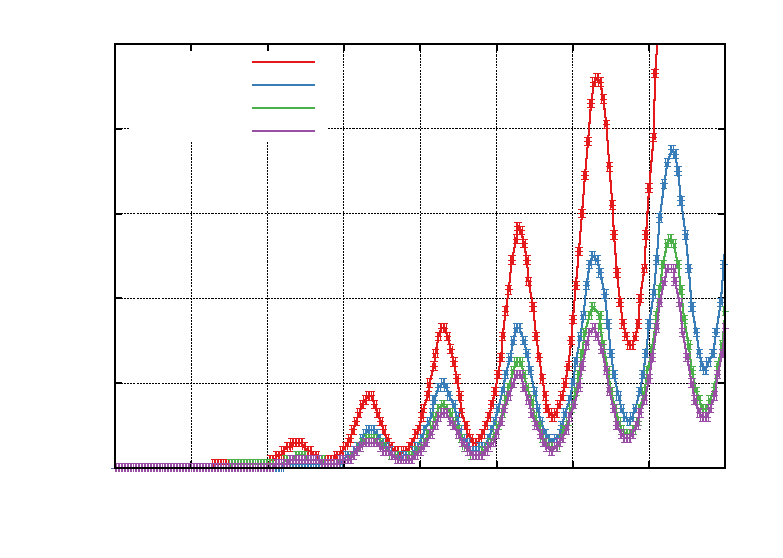
\includegraphics{./plots/fh_vartemp}}%
    \gplfronttext
  \end{picture}%
\endgroup

\caption{Variable Temperatur bei $\Delta U=\SI{2}{\volt}$ Gegenspannung}
\label{fig:fh_vartemp}
\end{figure}

\subsection{Auswertung}

\subsubsection{Energiedifferenz zwischen 6S- und 6P-Niveau in Quecksilber}

Zur Bestimmung der Energiedifferenz $\Delta E$ fitten wir mit gnuplot Gaußkurven an die Daten.
Als Fithypothese wählen wir dabei
\begin{align*}
\mathcal{G}_i(x)=A\,\exp\left[-\frac{1}{2}\left(\frac{x-S_i}{b}\right)^2\right] + c
\end{align*}
mit dem Peakschwerpunkt $S_i$, den wir zur Auswertung benötigen.
Wir lassen die Parameter nun an jeweils 4 Maxima pro Datensatz anpassen, wobei wir die Maxima mit $i$ von links nach rechts durchnummerieren, beginnend bei dem Maximum zwischen \SI{15}{\kilo\volt} und \SI{20}{\kilo\volt}, da das davor liegende Maximum besonders für hohe Gegenspannungen und hohe Temperaturen nicht gut gefittet werden kann.
Die Ergebnisse für die Schwerpunkte $S_i$ sind in Tabelle \ref{tab:fh_schwerpunkte} dargestellt, sowie bereits die Mittelwerte und deren (über die Standardabweichung bestimmten) Fehler für jeden Datensatz.
Nun mitteln wir diese Werte erneut, um einen Gesamtwert für den Energieabstand $\Delta E$ zu erhalten.
\begin{align*}
\Delta E = \SI{4.922+-0.021}{\electronvolt}
\end{align*}

\begin{table}[h]
\centering
\resizebox{\columnwidth}{!}{%
\begin{tabular}{llllll}
\toprule
$\Delta$U / \si{\volt} & $S_1$ / \si{\kilo\volt} & $S_2$ / \si{\kilo\volt} & $S_3$ / \si{\kilo\volt} & $S_4$ / \si{\kilo\volt} & Mittelwert\\
\midrule
\num{2.0} &	\num{16.63+-0.02} & \num{21.45+-0.02} &	\num{26.42+-0.01} &	\num{31.44+-0.02} &	\num{4.94+-0.06}\\
\num{2.5} &	\num{16.77+-0.02} &	\num{21.59+-0.01} &	\num{26.58+-0.01} &	\num{31.61+-0.01} &	\num{4.95+-0.07}\\
\num{3.0} &	\num{16.92+-0.03} &	\num{21.68+-0.02} &	\num{26.71+-0.02} &	\num{31.74+-0.01} &	\num{4.94+-0.09}\\
\num{3.5} &	\num{16.99+-0.05} &	\num{21.83+-0.03} &	\num{26.84+-0.02} &	\num{31.90+-0.02} &	\num{4.97+-0.07}\\
	      &					  &			  	 	  &					  &					  &					\\
{T / \si{\degreeCelsius}} & & & & & \\
\midrule
\num{155} &	\num{16.61+-0.02} &	\num{21.52+-0.02} &	\num{26.51+-0.02} &	\num{31.63+-0.02} &	\num{5.01+-0.07}\\
\num{160} &	\num{16.81+-0.04} &	\num{21.51+-0.02} &	\num{26.43+-0.02} &	\num{31.43+-0.02} &	\num{4.87+-0.10}\\
\num{165} &	\num{16.82+-0.04} &	\num{21.55+-0.02} &	\num{26.42+-0.02} &	\num{31.36+-0.02} &	\num{4.85+-0.07}\\
\num{170} &	\num{16.82+-0.05} &	\num{21.60+-0.02} &	\num{26.40+-0.02} &	\num{31.36+-0.02} &	\num{4.85+-0.06}\\
\bottomrule
\end{tabular}}
\caption{Messwerte der Peakschwerpunkte}
\label{tab:fh_schwerpunkte}
\end{table}

Um diesen Wert zu verstehen, muss man das Termschema und den Wirkungsquerschnitt bei Elektronenstoßanregung von Quecksilber betrachten.
In der Grafik zu letzterem sieht man vier Wirkungsquerschnitte für verschiedene Übergänge im Quecksilber in Abhängigkeit von den stoßenden Elektronen.
Da Linie 4 erst knapp unter \SI{20}{\electronvolt} ihr Maximum hat, Stöße offensichtlich aber auch schon bei geringen Energien stattfinden, werden wir diese nicht weiter beachten.
Genauso ignorieren wir Linie 1, da der maximale Wirkungsquerschnitt hier sehr gering ist im Vergleich zu den anderen in Betracht kommenden Linien 2 und 3.

Wir betrachten zur weiteren Auswertung also nur noch die Linien 2 und 3, wobei wir davon ausgehen können, dass der Wirkungsquerschnitt von Linie 2 ausreicht, um Stöße der Elektronen mit den Quecksilberatomen auszulösen.
Ein Argument für diese Annahme ist, dass die Linie bei geringeren Energien als Linie 3 sowohl beginnt, als auch ihr Maximum erreicht.
Die Linie 2 korrespondiert mit dem Übergang $6^1$S$_0\rightarrow6^3$P$_1$, so dass dieser am häufigsten stattfinden wird.
Dennoch können einige Elektronen bei dieser Energie keine Stöße ausführen und werden weiter beschleunigt, so dass diese erst gemäß Linie 3 Stöße ausführen können.
Darum wird der Übergang $6^1$S$_0\rightarrow6^3$P$_2$ in den Messwerten auch zu finden sein.

Zusammen mit dem Termschema, mit dem der Linie 2 die Energie \SI{4.89}{\electronvolt} und Linie 3 die Energie \SI{5.46}{\electronvolt} zugeordnet werden kann, erklärt sich damit die gefundene Energiedifferenz von $\Delta E = \SI{4.922+-0.021}{\electronvolt}$.
Diese liegt knapp über dem Wert von \SI{4.89}{\electronvolt}, da nebem diesem Übergang in Quecksilber auch einer mit \SI{5.46}{\electronvolt} stattfindet, allerdings deutlich seltener.

EVTL BERECHNNG WIE HAUER feat. DIETER

\subsubsection{Abhängigkeit des Anodenstroms von der Gegenspannung bzw. Temperatur}



\subsection{Diskussion}

% BIBLIOGRAPHIE

% Maximale Anzahl der Einträge in Klammer
% Zitieren mit \cite{lamport94}
\begin{thebibliography}{9}

% Beispiel
\bibitem{np_richardson}
 Nobelprize.org,
 \emph{"The Nobel Prize in Physics 1928"}.
 Nobel Media AB 2014. Web. 15\\
 (\url{http://www.nobelprize.org/nobel_prizes/physics/laureates/1928/richardson-lecture.pdf} abgerufen am 15.11.2014)
  
\bibitem{demtroeder3}
	Wolfgang Demtröder,
	\emph{Experimentalphysik 3}.
	Springer Verlag,
	3. Auflage
\end{thebibliography}

% APPENDIX
\begin{appendix}
\newpage
\section{Darstellung der Aufspaltung beim Zeeman-Effekt}

\begin{figure}[h]
\centering
% GNUPLOT: LaTeX picture with Postscript
\begingroup
  \makeatletter
  \providecommand\color[2][]{%
    \GenericError{(gnuplot) \space\space\space\@spaces}{%
      Package color not loaded in conjunction with
      terminal option `colourtext'%
    }{See the gnuplot documentation for explanation.%
    }{Either use 'blacktext' in gnuplot or load the package
      color.sty in LaTeX.}%
    \renewcommand\color[2][]{}%
  }%
  \providecommand\includegraphics[2][]{%
    \GenericError{(gnuplot) \space\space\space\@spaces}{%
      Package graphicx or graphics not loaded%
    }{See the gnuplot documentation for explanation.%
    }{The gnuplot epslatex terminal needs graphicx.sty or graphics.sty.}%
    \renewcommand\includegraphics[2][]{}%
  }%
  \providecommand\rotatebox[2]{#2}%
  \@ifundefined{ifGPcolor}{%
    \newif\ifGPcolor
    \GPcolortrue
  }{}%
  \@ifundefined{ifGPblacktext}{%
    \newif\ifGPblacktext
    \GPblacktexttrue
  }{}%
  % define a \g@addto@macro without @ in the name:
  \let\gplgaddtomacro\g@addto@macro
  % define empty templates for all commands taking text:
  \gdef\gplbacktext{}%
  \gdef\gplfronttext{}%
  \makeatother
  \ifGPblacktext
    % no textcolor at all
    \def\colorrgb#1{}%
    \def\colorgray#1{}%
  \else
    % gray or color?
    \ifGPcolor
      \def\colorrgb#1{\color[rgb]{#1}}%
      \def\colorgray#1{\color[gray]{#1}}%
      \expandafter\def\csname LTw\endcsname{\color{white}}%
      \expandafter\def\csname LTb\endcsname{\color{black}}%
      \expandafter\def\csname LTa\endcsname{\color{black}}%
      \expandafter\def\csname LT0\endcsname{\color[rgb]{1,0,0}}%
      \expandafter\def\csname LT1\endcsname{\color[rgb]{0,1,0}}%
      \expandafter\def\csname LT2\endcsname{\color[rgb]{0,0,1}}%
      \expandafter\def\csname LT3\endcsname{\color[rgb]{1,0,1}}%
      \expandafter\def\csname LT4\endcsname{\color[rgb]{0,1,1}}%
      \expandafter\def\csname LT5\endcsname{\color[rgb]{1,1,0}}%
      \expandafter\def\csname LT6\endcsname{\color[rgb]{0,0,0}}%
      \expandafter\def\csname LT7\endcsname{\color[rgb]{1,0.3,0}}%
      \expandafter\def\csname LT8\endcsname{\color[rgb]{0.5,0.5,0.5}}%
    \else
      % gray
      \def\colorrgb#1{\color{black}}%
      \def\colorgray#1{\color[gray]{#1}}%
      \expandafter\def\csname LTw\endcsname{\color{white}}%
      \expandafter\def\csname LTb\endcsname{\color{black}}%
      \expandafter\def\csname LTa\endcsname{\color{black}}%
      \expandafter\def\csname LT0\endcsname{\color{black}}%
      \expandafter\def\csname LT1\endcsname{\color{black}}%
      \expandafter\def\csname LT2\endcsname{\color{black}}%
      \expandafter\def\csname LT3\endcsname{\color{black}}%
      \expandafter\def\csname LT4\endcsname{\color{black}}%
      \expandafter\def\csname LT5\endcsname{\color{black}}%
      \expandafter\def\csname LT6\endcsname{\color{black}}%
      \expandafter\def\csname LT7\endcsname{\color{black}}%
      \expandafter\def\csname LT8\endcsname{\color{black}}%
    \fi
  \fi
  \setlength{\unitlength}{0.0500bp}%
  \begin{picture}(7486.00,5040.00)%
    \gplgaddtomacro\gplbacktext{%
      \csname LTb\endcsname%
      \put(814,704){\makebox(0,0)[r]{\strut{} 0}}%
      \csname LTb\endcsname%
      \put(814,1156){\makebox(0,0)[r]{\strut{} 5}}%
      \csname LTb\endcsname%
      \put(814,1609){\makebox(0,0)[r]{\strut{} 10}}%
      \csname LTb\endcsname%
      \put(814,2061){\makebox(0,0)[r]{\strut{} 15}}%
      \csname LTb\endcsname%
      \put(814,2513){\makebox(0,0)[r]{\strut{} 20}}%
      \csname LTb\endcsname%
      \put(814,2966){\makebox(0,0)[r]{\strut{} 25}}%
      \csname LTb\endcsname%
      \put(814,3418){\makebox(0,0)[r]{\strut{} 30}}%
      \csname LTb\endcsname%
      \put(814,3870){\makebox(0,0)[r]{\strut{} 35}}%
      \csname LTb\endcsname%
      \put(814,4323){\makebox(0,0)[r]{\strut{} 40}}%
      \csname LTb\endcsname%
      \put(814,4775){\makebox(0,0)[r]{\strut{} 45}}%
      \csname LTb\endcsname%
      \put(946,484){\makebox(0,0){\strut{} 0.8}}%
      \csname LTb\endcsname%
      \put(1714,484){\makebox(0,0){\strut{} 0.85}}%
      \csname LTb\endcsname%
      \put(2482,484){\makebox(0,0){\strut{} 0.9}}%
      \csname LTb\endcsname%
      \put(3250,484){\makebox(0,0){\strut{} 0.95}}%
      \csname LTb\endcsname%
      \put(4018,484){\makebox(0,0){\strut{} 1}}%
      \csname LTb\endcsname%
      \put(4785,484){\makebox(0,0){\strut{} 1.05}}%
      \csname LTb\endcsname%
      \put(5553,484){\makebox(0,0){\strut{} 1.1}}%
      \csname LTb\endcsname%
      \put(6321,484){\makebox(0,0){\strut{} 1.15}}%
      \csname LTb\endcsname%
      \put(7089,484){\makebox(0,0){\strut{} 1.2}}%
      \put(176,2739){\rotatebox{-270}{\makebox(0,0){\strut{}Intensität $I$ / \si{\percent}}}}%
      \put(4017,154){\makebox(0,0){\strut{}Winkel $\alpha$ / \si{\degree}}}%
      \put(4017,4665){\makebox(0,0){\strut{}}}%
    }%
    \gplgaddtomacro\gplfronttext{%
      \csname LTb\endcsname%
      \put(6102,4602){\makebox(0,0)[r]{\strut{}Messwerte}}%
      \csname LTb\endcsname%
      \put(6102,4382){\makebox(0,0)[r]{\strut{}Summe Gaußfits}}%
      \csname LTb\endcsname%
      \put(6102,4162){\makebox(0,0)[r]{\strut{}Funktion 1}}%
      \csname LTb\endcsname%
      \put(6102,3942){\makebox(0,0)[r]{\strut{}Funktion 2}}%
      \csname LTb\endcsname%
      \put(6102,3722){\makebox(0,0)[r]{\strut{}Funktion 3}}%
      \csname LTb\endcsname%
      \put(6102,3502){\makebox(0,0)[r]{\strut{}Untergrund}}%
    }%
    \gplbacktext
    \put(0,0){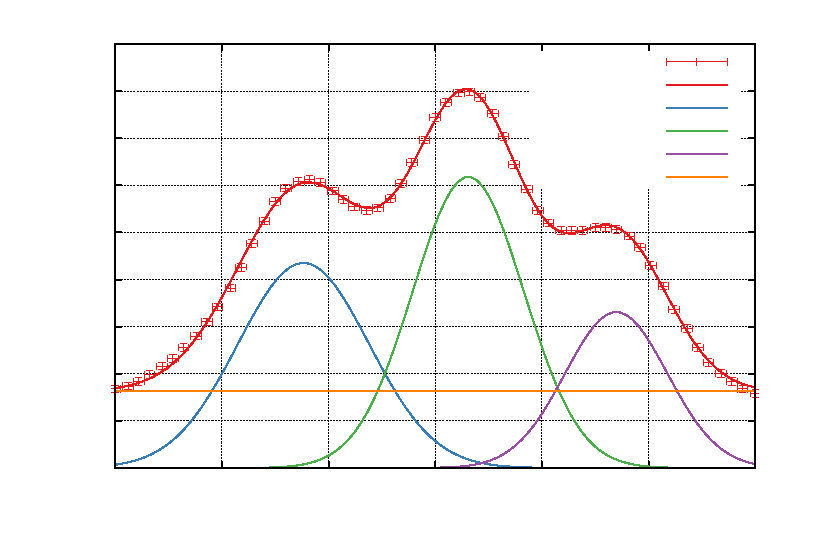
\includegraphics{./plots/zeemann_aufspaltung/b4}}%
    \gplfronttext
  \end{picture}%
\endgroup

\caption{4 A}
\label{fig:gauss1}
\end{figure}

\begin{figure}[h]
\centering
% GNUPLOT: LaTeX picture with Postscript
\begingroup
  \makeatletter
  \providecommand\color[2][]{%
    \GenericError{(gnuplot) \space\space\space\@spaces}{%
      Package color not loaded in conjunction with
      terminal option `colourtext'%
    }{See the gnuplot documentation for explanation.%
    }{Either use 'blacktext' in gnuplot or load the package
      color.sty in LaTeX.}%
    \renewcommand\color[2][]{}%
  }%
  \providecommand\includegraphics[2][]{%
    \GenericError{(gnuplot) \space\space\space\@spaces}{%
      Package graphicx or graphics not loaded%
    }{See the gnuplot documentation for explanation.%
    }{The gnuplot epslatex terminal needs graphicx.sty or graphics.sty.}%
    \renewcommand\includegraphics[2][]{}%
  }%
  \providecommand\rotatebox[2]{#2}%
  \@ifundefined{ifGPcolor}{%
    \newif\ifGPcolor
    \GPcolortrue
  }{}%
  \@ifundefined{ifGPblacktext}{%
    \newif\ifGPblacktext
    \GPblacktexttrue
  }{}%
  % define a \g@addto@macro without @ in the name:
  \let\gplgaddtomacro\g@addto@macro
  % define empty templates for all commands taking text:
  \gdef\gplbacktext{}%
  \gdef\gplfronttext{}%
  \makeatother
  \ifGPblacktext
    % no textcolor at all
    \def\colorrgb#1{}%
    \def\colorgray#1{}%
  \else
    % gray or color?
    \ifGPcolor
      \def\colorrgb#1{\color[rgb]{#1}}%
      \def\colorgray#1{\color[gray]{#1}}%
      \expandafter\def\csname LTw\endcsname{\color{white}}%
      \expandafter\def\csname LTb\endcsname{\color{black}}%
      \expandafter\def\csname LTa\endcsname{\color{black}}%
      \expandafter\def\csname LT0\endcsname{\color[rgb]{1,0,0}}%
      \expandafter\def\csname LT1\endcsname{\color[rgb]{0,1,0}}%
      \expandafter\def\csname LT2\endcsname{\color[rgb]{0,0,1}}%
      \expandafter\def\csname LT3\endcsname{\color[rgb]{1,0,1}}%
      \expandafter\def\csname LT4\endcsname{\color[rgb]{0,1,1}}%
      \expandafter\def\csname LT5\endcsname{\color[rgb]{1,1,0}}%
      \expandafter\def\csname LT6\endcsname{\color[rgb]{0,0,0}}%
      \expandafter\def\csname LT7\endcsname{\color[rgb]{1,0.3,0}}%
      \expandafter\def\csname LT8\endcsname{\color[rgb]{0.5,0.5,0.5}}%
    \else
      % gray
      \def\colorrgb#1{\color{black}}%
      \def\colorgray#1{\color[gray]{#1}}%
      \expandafter\def\csname LTw\endcsname{\color{white}}%
      \expandafter\def\csname LTb\endcsname{\color{black}}%
      \expandafter\def\csname LTa\endcsname{\color{black}}%
      \expandafter\def\csname LT0\endcsname{\color{black}}%
      \expandafter\def\csname LT1\endcsname{\color{black}}%
      \expandafter\def\csname LT2\endcsname{\color{black}}%
      \expandafter\def\csname LT3\endcsname{\color{black}}%
      \expandafter\def\csname LT4\endcsname{\color{black}}%
      \expandafter\def\csname LT5\endcsname{\color{black}}%
      \expandafter\def\csname LT6\endcsname{\color{black}}%
      \expandafter\def\csname LT7\endcsname{\color{black}}%
      \expandafter\def\csname LT8\endcsname{\color{black}}%
    \fi
  \fi
  \setlength{\unitlength}{0.0500bp}%
  \begin{picture}(7488.00,5040.00)%
    \gplgaddtomacro\gplbacktext{%
      \csname LTb\endcsname%
      \put(814,704){\makebox(0,0)[r]{\strut{} 0}}%
      \csname LTb\endcsname%
      \put(814,1156){\makebox(0,0)[r]{\strut{} 5}}%
      \csname LTb\endcsname%
      \put(814,1609){\makebox(0,0)[r]{\strut{} 10}}%
      \csname LTb\endcsname%
      \put(814,2061){\makebox(0,0)[r]{\strut{} 15}}%
      \csname LTb\endcsname%
      \put(814,2513){\makebox(0,0)[r]{\strut{} 20}}%
      \csname LTb\endcsname%
      \put(814,2966){\makebox(0,0)[r]{\strut{} 25}}%
      \csname LTb\endcsname%
      \put(814,3418){\makebox(0,0)[r]{\strut{} 30}}%
      \csname LTb\endcsname%
      \put(814,3870){\makebox(0,0)[r]{\strut{} 35}}%
      \csname LTb\endcsname%
      \put(814,4323){\makebox(0,0)[r]{\strut{} 40}}%
      \csname LTb\endcsname%
      \put(814,4775){\makebox(0,0)[r]{\strut{} 45}}%
      \csname LTb\endcsname%
      \put(1438,484){\makebox(0,0){\strut{} 0.9}}%
      \csname LTb\endcsname%
      \put(2667,484){\makebox(0,0){\strut{} 0.95}}%
      \csname LTb\endcsname%
      \put(3896,484){\makebox(0,0){\strut{} 1}}%
      \csname LTb\endcsname%
      \put(5125,484){\makebox(0,0){\strut{} 1.05}}%
      \csname LTb\endcsname%
      \put(6354,484){\makebox(0,0){\strut{} 1.1}}%
      \put(176,2739){\rotatebox{-270}{\makebox(0,0){\strut{}Intensität $I$ / \si{\percent}}}}%
      \put(4018,154){\makebox(0,0){\strut{}Winkel $\alpha$ / \si{\degree}}}%
      \put(4018,4665){\makebox(0,0){\strut{}}}%
    }%
    \gplgaddtomacro\gplfronttext{%
      \csname LTb\endcsname%
      \put(6104,4602){\makebox(0,0)[r]{\strut{}Messwerte}}%
      \csname LTb\endcsname%
      \put(6104,4382){\makebox(0,0)[r]{\strut{}$\Sigma$}}%
      \csname LTb\endcsname%
      \put(6104,4162){\makebox(0,0)[r]{\strut{}$\mathcal{G}_1$}}%
      \csname LTb\endcsname%
      \put(6104,3942){\makebox(0,0)[r]{\strut{}$\mathcal{G}_2$}}%
      \csname LTb\endcsname%
      \put(6104,3722){\makebox(0,0)[r]{\strut{}$\mathcal{G}_3$}}%
      \csname LTb\endcsname%
      \put(6104,3502){\makebox(0,0)[r]{\strut{}Untergrund}}%
    }%
    \gplbacktext
    \put(0,0){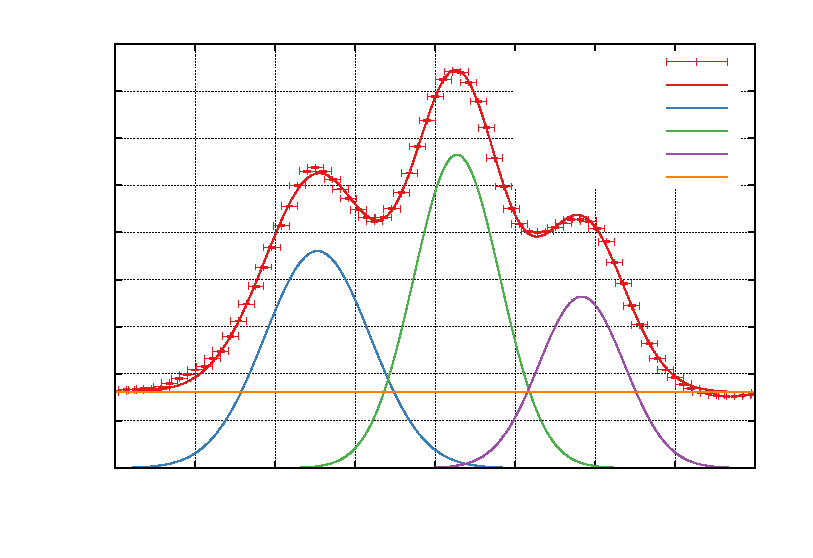
\includegraphics{./plots/zeemann_aufspaltung/b4-5}}%
    \gplfronttext
  \end{picture}%
\endgroup

\caption{4.5 A}
\label{fig:gauss2}
\end{figure}

\begin{figure}[h]
\centering
% GNUPLOT: LaTeX picture with Postscript
\begingroup
  \makeatletter
  \providecommand\color[2][]{%
    \GenericError{(gnuplot) \space\space\space\@spaces}{%
      Package color not loaded in conjunction with
      terminal option `colourtext'%
    }{See the gnuplot documentation for explanation.%
    }{Either use 'blacktext' in gnuplot or load the package
      color.sty in LaTeX.}%
    \renewcommand\color[2][]{}%
  }%
  \providecommand\includegraphics[2][]{%
    \GenericError{(gnuplot) \space\space\space\@spaces}{%
      Package graphicx or graphics not loaded%
    }{See the gnuplot documentation for explanation.%
    }{The gnuplot epslatex terminal needs graphicx.sty or graphics.sty.}%
    \renewcommand\includegraphics[2][]{}%
  }%
  \providecommand\rotatebox[2]{#2}%
  \@ifundefined{ifGPcolor}{%
    \newif\ifGPcolor
    \GPcolortrue
  }{}%
  \@ifundefined{ifGPblacktext}{%
    \newif\ifGPblacktext
    \GPblacktexttrue
  }{}%
  % define a \g@addto@macro without @ in the name:
  \let\gplgaddtomacro\g@addto@macro
  % define empty templates for all commands taking text:
  \gdef\gplbacktext{}%
  \gdef\gplfronttext{}%
  \makeatother
  \ifGPblacktext
    % no textcolor at all
    \def\colorrgb#1{}%
    \def\colorgray#1{}%
  \else
    % gray or color?
    \ifGPcolor
      \def\colorrgb#1{\color[rgb]{#1}}%
      \def\colorgray#1{\color[gray]{#1}}%
      \expandafter\def\csname LTw\endcsname{\color{white}}%
      \expandafter\def\csname LTb\endcsname{\color{black}}%
      \expandafter\def\csname LTa\endcsname{\color{black}}%
      \expandafter\def\csname LT0\endcsname{\color[rgb]{1,0,0}}%
      \expandafter\def\csname LT1\endcsname{\color[rgb]{0,1,0}}%
      \expandafter\def\csname LT2\endcsname{\color[rgb]{0,0,1}}%
      \expandafter\def\csname LT3\endcsname{\color[rgb]{1,0,1}}%
      \expandafter\def\csname LT4\endcsname{\color[rgb]{0,1,1}}%
      \expandafter\def\csname LT5\endcsname{\color[rgb]{1,1,0}}%
      \expandafter\def\csname LT6\endcsname{\color[rgb]{0,0,0}}%
      \expandafter\def\csname LT7\endcsname{\color[rgb]{1,0.3,0}}%
      \expandafter\def\csname LT8\endcsname{\color[rgb]{0.5,0.5,0.5}}%
    \else
      % gray
      \def\colorrgb#1{\color{black}}%
      \def\colorgray#1{\color[gray]{#1}}%
      \expandafter\def\csname LTw\endcsname{\color{white}}%
      \expandafter\def\csname LTb\endcsname{\color{black}}%
      \expandafter\def\csname LTa\endcsname{\color{black}}%
      \expandafter\def\csname LT0\endcsname{\color{black}}%
      \expandafter\def\csname LT1\endcsname{\color{black}}%
      \expandafter\def\csname LT2\endcsname{\color{black}}%
      \expandafter\def\csname LT3\endcsname{\color{black}}%
      \expandafter\def\csname LT4\endcsname{\color{black}}%
      \expandafter\def\csname LT5\endcsname{\color{black}}%
      \expandafter\def\csname LT6\endcsname{\color{black}}%
      \expandafter\def\csname LT7\endcsname{\color{black}}%
      \expandafter\def\csname LT8\endcsname{\color{black}}%
    \fi
  \fi
  \setlength{\unitlength}{0.0500bp}%
  \begin{picture}(7488.00,5040.00)%
    \gplgaddtomacro\gplbacktext{%
      \csname LTb\endcsname%
      \put(814,704){\makebox(0,0)[r]{\strut{} 0}}%
      \csname LTb\endcsname%
      \put(814,1156){\makebox(0,0)[r]{\strut{} 5}}%
      \csname LTb\endcsname%
      \put(814,1609){\makebox(0,0)[r]{\strut{} 10}}%
      \csname LTb\endcsname%
      \put(814,2061){\makebox(0,0)[r]{\strut{} 15}}%
      \csname LTb\endcsname%
      \put(814,2513){\makebox(0,0)[r]{\strut{} 20}}%
      \csname LTb\endcsname%
      \put(814,2966){\makebox(0,0)[r]{\strut{} 25}}%
      \csname LTb\endcsname%
      \put(814,3418){\makebox(0,0)[r]{\strut{} 30}}%
      \csname LTb\endcsname%
      \put(814,3870){\makebox(0,0)[r]{\strut{} 35}}%
      \csname LTb\endcsname%
      \put(814,4323){\makebox(0,0)[r]{\strut{} 40}}%
      \csname LTb\endcsname%
      \put(814,4775){\makebox(0,0)[r]{\strut{} 45}}%
      \csname LTb\endcsname%
      \put(1655,484){\makebox(0,0){\strut{} 0.9}}%
      \csname LTb\endcsname%
      \put(2837,484){\makebox(0,0){\strut{} 0.95}}%
      \csname LTb\endcsname%
      \put(4019,484){\makebox(0,0){\strut{} 1}}%
      \csname LTb\endcsname%
      \put(5200,484){\makebox(0,0){\strut{} 1.05}}%
      \csname LTb\endcsname%
      \put(6382,484){\makebox(0,0){\strut{} 1.1}}%
      \put(176,2739){\rotatebox{-270}{\makebox(0,0){\strut{}Intensität $I$ / \si{\percent}}}}%
      \put(4018,154){\makebox(0,0){\strut{}Winkel $\alpha$ / \si{\degree}}}%
      \put(4018,4665){\makebox(0,0){\strut{}}}%
    }%
    \gplgaddtomacro\gplfronttext{%
      \csname LTb\endcsname%
      \put(6104,4602){\makebox(0,0)[r]{\strut{}Messwerte}}%
      \csname LTb\endcsname%
      \put(6104,4382){\makebox(0,0)[r]{\strut{}$\Sigma$}}%
      \csname LTb\endcsname%
      \put(6104,4162){\makebox(0,0)[r]{\strut{}$\mathcal{G}_1$}}%
      \csname LTb\endcsname%
      \put(6104,3942){\makebox(0,0)[r]{\strut{}$\mathcal{G}_2$}}%
      \csname LTb\endcsname%
      \put(6104,3722){\makebox(0,0)[r]{\strut{}$\mathcal{G}_3$}}%
      \csname LTb\endcsname%
      \put(6104,3502){\makebox(0,0)[r]{\strut{}Untergrund}}%
    }%
    \gplbacktext
    \put(0,0){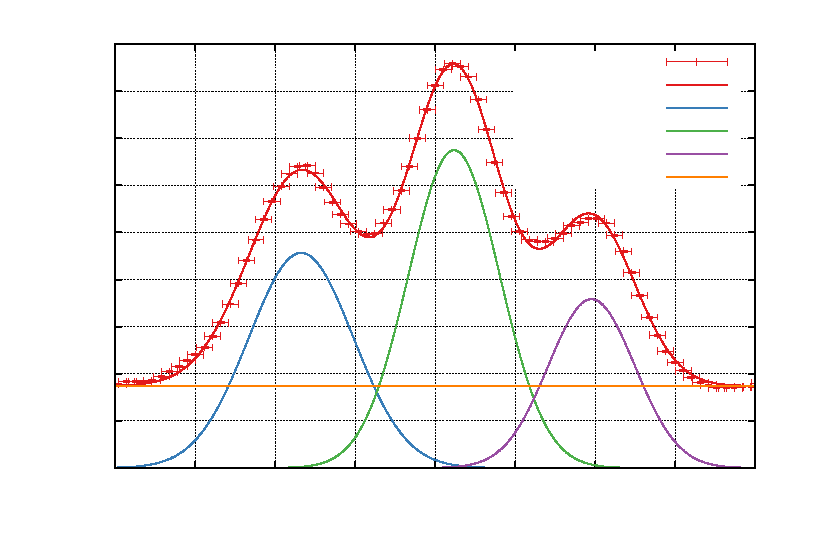
\includegraphics{./plots/zeemann_aufspaltung/b5}}%
    \gplfronttext
  \end{picture}%
\endgroup

\caption{5A}
\label{fig:gauss3}
\end{figure}

\begin{figure}[h]
\centering
% GNUPLOT: LaTeX picture with Postscript
\begingroup
  \makeatletter
  \providecommand\color[2][]{%
    \GenericError{(gnuplot) \space\space\space\@spaces}{%
      Package color not loaded in conjunction with
      terminal option `colourtext'%
    }{See the gnuplot documentation for explanation.%
    }{Either use 'blacktext' in gnuplot or load the package
      color.sty in LaTeX.}%
    \renewcommand\color[2][]{}%
  }%
  \providecommand\includegraphics[2][]{%
    \GenericError{(gnuplot) \space\space\space\@spaces}{%
      Package graphicx or graphics not loaded%
    }{See the gnuplot documentation for explanation.%
    }{The gnuplot epslatex terminal needs graphicx.sty or graphics.sty.}%
    \renewcommand\includegraphics[2][]{}%
  }%
  \providecommand\rotatebox[2]{#2}%
  \@ifundefined{ifGPcolor}{%
    \newif\ifGPcolor
    \GPcolortrue
  }{}%
  \@ifundefined{ifGPblacktext}{%
    \newif\ifGPblacktext
    \GPblacktexttrue
  }{}%
  % define a \g@addto@macro without @ in the name:
  \let\gplgaddtomacro\g@addto@macro
  % define empty templates for all commands taking text:
  \gdef\gplbacktext{}%
  \gdef\gplfronttext{}%
  \makeatother
  \ifGPblacktext
    % no textcolor at all
    \def\colorrgb#1{}%
    \def\colorgray#1{}%
  \else
    % gray or color?
    \ifGPcolor
      \def\colorrgb#1{\color[rgb]{#1}}%
      \def\colorgray#1{\color[gray]{#1}}%
      \expandafter\def\csname LTw\endcsname{\color{white}}%
      \expandafter\def\csname LTb\endcsname{\color{black}}%
      \expandafter\def\csname LTa\endcsname{\color{black}}%
      \expandafter\def\csname LT0\endcsname{\color[rgb]{1,0,0}}%
      \expandafter\def\csname LT1\endcsname{\color[rgb]{0,1,0}}%
      \expandafter\def\csname LT2\endcsname{\color[rgb]{0,0,1}}%
      \expandafter\def\csname LT3\endcsname{\color[rgb]{1,0,1}}%
      \expandafter\def\csname LT4\endcsname{\color[rgb]{0,1,1}}%
      \expandafter\def\csname LT5\endcsname{\color[rgb]{1,1,0}}%
      \expandafter\def\csname LT6\endcsname{\color[rgb]{0,0,0}}%
      \expandafter\def\csname LT7\endcsname{\color[rgb]{1,0.3,0}}%
      \expandafter\def\csname LT8\endcsname{\color[rgb]{0.5,0.5,0.5}}%
    \else
      % gray
      \def\colorrgb#1{\color{black}}%
      \def\colorgray#1{\color[gray]{#1}}%
      \expandafter\def\csname LTw\endcsname{\color{white}}%
      \expandafter\def\csname LTb\endcsname{\color{black}}%
      \expandafter\def\csname LTa\endcsname{\color{black}}%
      \expandafter\def\csname LT0\endcsname{\color{black}}%
      \expandafter\def\csname LT1\endcsname{\color{black}}%
      \expandafter\def\csname LT2\endcsname{\color{black}}%
      \expandafter\def\csname LT3\endcsname{\color{black}}%
      \expandafter\def\csname LT4\endcsname{\color{black}}%
      \expandafter\def\csname LT5\endcsname{\color{black}}%
      \expandafter\def\csname LT6\endcsname{\color{black}}%
      \expandafter\def\csname LT7\endcsname{\color{black}}%
      \expandafter\def\csname LT8\endcsname{\color{black}}%
    \fi
  \fi
  \setlength{\unitlength}{0.0500bp}%
  \begin{picture}(7486.00,5040.00)%
    \gplgaddtomacro\gplbacktext{%
      \csname LTb\endcsname%
      \put(814,704){\makebox(0,0)[r]{\strut{} 0}}%
      \csname LTb\endcsname%
      \put(814,1156){\makebox(0,0)[r]{\strut{} 5}}%
      \csname LTb\endcsname%
      \put(814,1609){\makebox(0,0)[r]{\strut{} 10}}%
      \csname LTb\endcsname%
      \put(814,2061){\makebox(0,0)[r]{\strut{} 15}}%
      \csname LTb\endcsname%
      \put(814,2513){\makebox(0,0)[r]{\strut{} 20}}%
      \csname LTb\endcsname%
      \put(814,2966){\makebox(0,0)[r]{\strut{} 25}}%
      \csname LTb\endcsname%
      \put(814,3418){\makebox(0,0)[r]{\strut{} 30}}%
      \csname LTb\endcsname%
      \put(814,3870){\makebox(0,0)[r]{\strut{} 35}}%
      \csname LTb\endcsname%
      \put(814,4323){\makebox(0,0)[r]{\strut{} 40}}%
      \csname LTb\endcsname%
      \put(814,4775){\makebox(0,0)[r]{\strut{} 45}}%
      \csname LTb\endcsname%
      \put(946,484){\makebox(0,0){\strut{} 0.8}}%
      \csname LTb\endcsname%
      \put(1714,484){\makebox(0,0){\strut{} 0.85}}%
      \csname LTb\endcsname%
      \put(2482,484){\makebox(0,0){\strut{} 0.9}}%
      \csname LTb\endcsname%
      \put(3250,484){\makebox(0,0){\strut{} 0.95}}%
      \csname LTb\endcsname%
      \put(4018,484){\makebox(0,0){\strut{} 1}}%
      \csname LTb\endcsname%
      \put(4785,484){\makebox(0,0){\strut{} 1.05}}%
      \csname LTb\endcsname%
      \put(5553,484){\makebox(0,0){\strut{} 1.1}}%
      \csname LTb\endcsname%
      \put(6321,484){\makebox(0,0){\strut{} 1.15}}%
      \csname LTb\endcsname%
      \put(7089,484){\makebox(0,0){\strut{} 1.2}}%
      \put(176,2739){\rotatebox{-270}{\makebox(0,0){\strut{}Intensität $I$ / \si{\percent}}}}%
      \put(4017,154){\makebox(0,0){\strut{}Winkel $\alpha$ / \si{\degree}}}%
      \put(4017,4665){\makebox(0,0){\strut{}}}%
    }%
    \gplgaddtomacro\gplfronttext{%
      \csname LTb\endcsname%
      \put(6102,4602){\makebox(0,0)[r]{\strut{}Messwerte}}%
      \csname LTb\endcsname%
      \put(6102,4382){\makebox(0,0)[r]{\strut{}$\Sigma$}}%
      \csname LTb\endcsname%
      \put(6102,4162){\makebox(0,0)[r]{\strut{}$\mathcal{G}_1$}}%
      \csname LTb\endcsname%
      \put(6102,3942){\makebox(0,0)[r]{\strut{}$\mathcal{G}_2$}}%
      \csname LTb\endcsname%
      \put(6102,3722){\makebox(0,0)[r]{\strut{}$\mathcal{G}_3$}}%
      \csname LTb\endcsname%
      \put(6102,3502){\makebox(0,0)[r]{\strut{}Untergrund}}%
    }%
    \gplbacktext
    \put(0,0){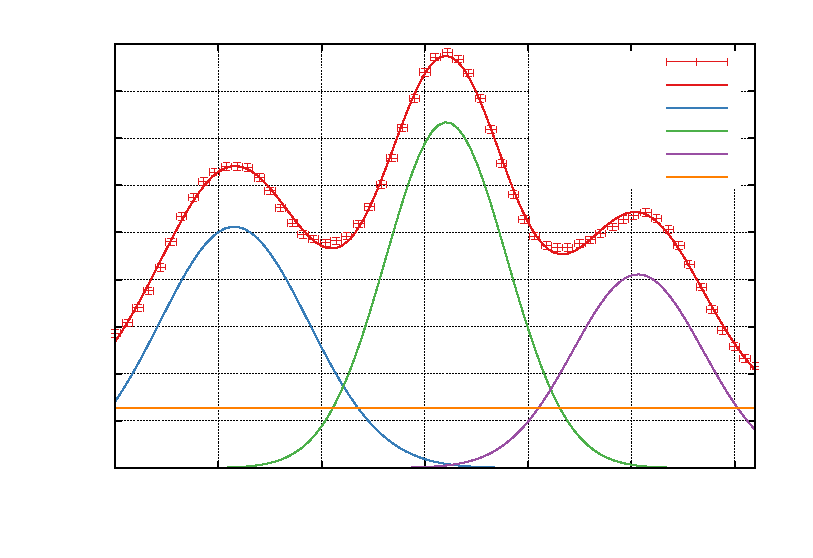
\includegraphics{./plots/zeemann_aufspaltung/b5-5}}%
    \gplfronttext
  \end{picture}%
\endgroup

\caption{5.5A}
\label{fig:gauss4}
\end{figure}

\begin{figure}[h]
\centering
% GNUPLOT: LaTeX picture with Postscript
\begingroup
  \makeatletter
  \providecommand\color[2][]{%
    \GenericError{(gnuplot) \space\space\space\@spaces}{%
      Package color not loaded in conjunction with
      terminal option `colourtext'%
    }{See the gnuplot documentation for explanation.%
    }{Either use 'blacktext' in gnuplot or load the package
      color.sty in LaTeX.}%
    \renewcommand\color[2][]{}%
  }%
  \providecommand\includegraphics[2][]{%
    \GenericError{(gnuplot) \space\space\space\@spaces}{%
      Package graphicx or graphics not loaded%
    }{See the gnuplot documentation for explanation.%
    }{The gnuplot epslatex terminal needs graphicx.sty or graphics.sty.}%
    \renewcommand\includegraphics[2][]{}%
  }%
  \providecommand\rotatebox[2]{#2}%
  \@ifundefined{ifGPcolor}{%
    \newif\ifGPcolor
    \GPcolortrue
  }{}%
  \@ifundefined{ifGPblacktext}{%
    \newif\ifGPblacktext
    \GPblacktexttrue
  }{}%
  % define a \g@addto@macro without @ in the name:
  \let\gplgaddtomacro\g@addto@macro
  % define empty templates for all commands taking text:
  \gdef\gplbacktext{}%
  \gdef\gplfronttext{}%
  \makeatother
  \ifGPblacktext
    % no textcolor at all
    \def\colorrgb#1{}%
    \def\colorgray#1{}%
  \else
    % gray or color?
    \ifGPcolor
      \def\colorrgb#1{\color[rgb]{#1}}%
      \def\colorgray#1{\color[gray]{#1}}%
      \expandafter\def\csname LTw\endcsname{\color{white}}%
      \expandafter\def\csname LTb\endcsname{\color{black}}%
      \expandafter\def\csname LTa\endcsname{\color{black}}%
      \expandafter\def\csname LT0\endcsname{\color[rgb]{1,0,0}}%
      \expandafter\def\csname LT1\endcsname{\color[rgb]{0,1,0}}%
      \expandafter\def\csname LT2\endcsname{\color[rgb]{0,0,1}}%
      \expandafter\def\csname LT3\endcsname{\color[rgb]{1,0,1}}%
      \expandafter\def\csname LT4\endcsname{\color[rgb]{0,1,1}}%
      \expandafter\def\csname LT5\endcsname{\color[rgb]{1,1,0}}%
      \expandafter\def\csname LT6\endcsname{\color[rgb]{0,0,0}}%
      \expandafter\def\csname LT7\endcsname{\color[rgb]{1,0.3,0}}%
      \expandafter\def\csname LT8\endcsname{\color[rgb]{0.5,0.5,0.5}}%
    \else
      % gray
      \def\colorrgb#1{\color{black}}%
      \def\colorgray#1{\color[gray]{#1}}%
      \expandafter\def\csname LTw\endcsname{\color{white}}%
      \expandafter\def\csname LTb\endcsname{\color{black}}%
      \expandafter\def\csname LTa\endcsname{\color{black}}%
      \expandafter\def\csname LT0\endcsname{\color{black}}%
      \expandafter\def\csname LT1\endcsname{\color{black}}%
      \expandafter\def\csname LT2\endcsname{\color{black}}%
      \expandafter\def\csname LT3\endcsname{\color{black}}%
      \expandafter\def\csname LT4\endcsname{\color{black}}%
      \expandafter\def\csname LT5\endcsname{\color{black}}%
      \expandafter\def\csname LT6\endcsname{\color{black}}%
      \expandafter\def\csname LT7\endcsname{\color{black}}%
      \expandafter\def\csname LT8\endcsname{\color{black}}%
    \fi
  \fi
  \setlength{\unitlength}{0.0500bp}%
  \begin{picture}(7486.00,5040.00)%
    \gplgaddtomacro\gplbacktext{%
      \csname LTb\endcsname%
      \put(814,704){\makebox(0,0)[r]{\strut{} 0}}%
      \csname LTb\endcsname%
      \put(814,1111){\makebox(0,0)[r]{\strut{} 5}}%
      \csname LTb\endcsname%
      \put(814,1518){\makebox(0,0)[r]{\strut{} 10}}%
      \csname LTb\endcsname%
      \put(814,1925){\makebox(0,0)[r]{\strut{} 15}}%
      \csname LTb\endcsname%
      \put(814,2332){\makebox(0,0)[r]{\strut{} 20}}%
      \csname LTb\endcsname%
      \put(814,2740){\makebox(0,0)[r]{\strut{} 25}}%
      \csname LTb\endcsname%
      \put(814,3147){\makebox(0,0)[r]{\strut{} 30}}%
      \csname LTb\endcsname%
      \put(814,3554){\makebox(0,0)[r]{\strut{} 35}}%
      \csname LTb\endcsname%
      \put(814,3961){\makebox(0,0)[r]{\strut{} 40}}%
      \csname LTb\endcsname%
      \put(814,4368){\makebox(0,0)[r]{\strut{} 45}}%
      \csname LTb\endcsname%
      \put(814,4775){\makebox(0,0)[r]{\strut{} 50}}%
      \csname LTb\endcsname%
      \put(946,484){\makebox(0,0){\strut{} 0.8}}%
      \csname LTb\endcsname%
      \put(1714,484){\makebox(0,0){\strut{} 0.85}}%
      \csname LTb\endcsname%
      \put(2482,484){\makebox(0,0){\strut{} 0.9}}%
      \csname LTb\endcsname%
      \put(3250,484){\makebox(0,0){\strut{} 0.95}}%
      \csname LTb\endcsname%
      \put(4018,484){\makebox(0,0){\strut{} 1}}%
      \csname LTb\endcsname%
      \put(4785,484){\makebox(0,0){\strut{} 1.05}}%
      \csname LTb\endcsname%
      \put(5553,484){\makebox(0,0){\strut{} 1.1}}%
      \csname LTb\endcsname%
      \put(6321,484){\makebox(0,0){\strut{} 1.15}}%
      \csname LTb\endcsname%
      \put(7089,484){\makebox(0,0){\strut{} 1.2}}%
      \put(176,2739){\rotatebox{-270}{\makebox(0,0){\strut{}Intensität $I$ / \si{\percent}}}}%
      \put(4017,154){\makebox(0,0){\strut{}Winkel $\alpha$ / \si{\degree}}}%
      \put(4017,4665){\makebox(0,0){\strut{}}}%
    }%
    \gplgaddtomacro\gplfronttext{%
      \csname LTb\endcsname%
      \put(6102,4602){\makebox(0,0)[r]{\strut{}Messwerte}}%
      \csname LTb\endcsname%
      \put(6102,4382){\makebox(0,0)[r]{\strut{}$\Sigma$}}%
      \csname LTb\endcsname%
      \put(6102,4162){\makebox(0,0)[r]{\strut{}$\mathcal{G}_1$}}%
      \csname LTb\endcsname%
      \put(6102,3942){\makebox(0,0)[r]{\strut{}$\mathcal{G}_2$}}%
      \csname LTb\endcsname%
      \put(6102,3722){\makebox(0,0)[r]{\strut{}$\mathcal{G}_3$}}%
      \csname LTb\endcsname%
      \put(6102,3502){\makebox(0,0)[r]{\strut{}Untergrund}}%
    }%
    \gplbacktext
    \put(0,0){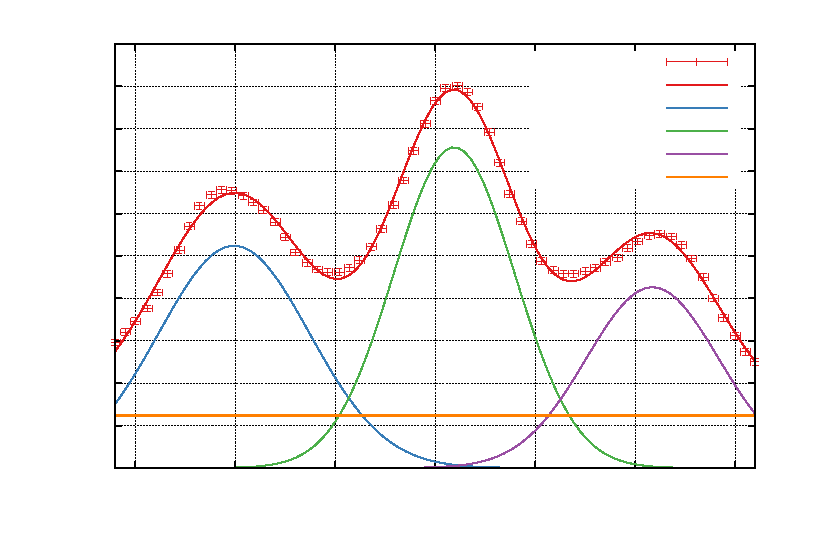
\includegraphics{./plots/zeemann_aufspaltung/b6}}%
    \gplfronttext
  \end{picture}%
\endgroup

\caption{6A}
\label{fig:gauss5}
\end{figure}

<<<<<<< HEAD
\section{Gaußfits}
\FloatBarrier

\begin{figure}[h]
	\centering
	% GNUPLOT: LaTeX picture with Postscript
\begingroup
  \makeatletter
  \providecommand\color[2][]{%
    \GenericError{(gnuplot) \space\space\space\@spaces}{%
      Package color not loaded in conjunction with
      terminal option `colourtext'%
    }{See the gnuplot documentation for explanation.%
    }{Either use 'blacktext' in gnuplot or load the package
      color.sty in LaTeX.}%
    \renewcommand\color[2][]{}%
  }%
  \providecommand\includegraphics[2][]{%
    \GenericError{(gnuplot) \space\space\space\@spaces}{%
      Package graphicx or graphics not loaded%
    }{See the gnuplot documentation for explanation.%
    }{The gnuplot epslatex terminal needs graphicx.sty or graphics.sty.}%
    \renewcommand\includegraphics[2][]{}%
  }%
  \providecommand\rotatebox[2]{#2}%
  \@ifundefined{ifGPcolor}{%
    \newif\ifGPcolor
    \GPcolortrue
  }{}%
  \@ifundefined{ifGPblacktext}{%
    \newif\ifGPblacktext
    \GPblacktexttrue
  }{}%
  % define a \g@addto@macro without @ in the name:
  \let\gplgaddtomacro\g@addto@macro
  % define empty templates for all commands taking text:
  \gdef\gplbacktext{}%
  \gdef\gplfronttext{}%
  \makeatother
  \ifGPblacktext
    % no textcolor at all
    \def\colorrgb#1{}%
    \def\colorgray#1{}%
  \else
    % gray or color?
    \ifGPcolor
      \def\colorrgb#1{\color[rgb]{#1}}%
      \def\colorgray#1{\color[gray]{#1}}%
      \expandafter\def\csname LTw\endcsname{\color{white}}%
      \expandafter\def\csname LTb\endcsname{\color{black}}%
      \expandafter\def\csname LTa\endcsname{\color{black}}%
      \expandafter\def\csname LT0\endcsname{\color[rgb]{1,0,0}}%
      \expandafter\def\csname LT1\endcsname{\color[rgb]{0,1,0}}%
      \expandafter\def\csname LT2\endcsname{\color[rgb]{0,0,1}}%
      \expandafter\def\csname LT3\endcsname{\color[rgb]{1,0,1}}%
      \expandafter\def\csname LT4\endcsname{\color[rgb]{0,1,1}}%
      \expandafter\def\csname LT5\endcsname{\color[rgb]{1,1,0}}%
      \expandafter\def\csname LT6\endcsname{\color[rgb]{0,0,0}}%
      \expandafter\def\csname LT7\endcsname{\color[rgb]{1,0.3,0}}%
      \expandafter\def\csname LT8\endcsname{\color[rgb]{0.5,0.5,0.5}}%
    \else
      % gray
      \def\colorrgb#1{\color{black}}%
      \def\colorgray#1{\color[gray]{#1}}%
      \expandafter\def\csname LTw\endcsname{\color{white}}%
      \expandafter\def\csname LTb\endcsname{\color{black}}%
      \expandafter\def\csname LTa\endcsname{\color{black}}%
      \expandafter\def\csname LT0\endcsname{\color{black}}%
      \expandafter\def\csname LT1\endcsname{\color{black}}%
      \expandafter\def\csname LT2\endcsname{\color{black}}%
      \expandafter\def\csname LT3\endcsname{\color{black}}%
      \expandafter\def\csname LT4\endcsname{\color{black}}%
      \expandafter\def\csname LT5\endcsname{\color{black}}%
      \expandafter\def\csname LT6\endcsname{\color{black}}%
      \expandafter\def\csname LT7\endcsname{\color{black}}%
      \expandafter\def\csname LT8\endcsname{\color{black}}%
    \fi
  \fi
  \setlength{\unitlength}{0.0500bp}%
  \begin{picture}(7486.00,5040.00)%
    \gplgaddtomacro\gplbacktext{%
      \csname LTb\endcsname%
      \put(814,704){\makebox(0,0)[r]{\strut{} 0}}%
      \csname LTb\endcsname%
      \put(814,1156){\makebox(0,0)[r]{\strut{} 5}}%
      \csname LTb\endcsname%
      \put(814,1609){\makebox(0,0)[r]{\strut{} 10}}%
      \csname LTb\endcsname%
      \put(814,2061){\makebox(0,0)[r]{\strut{} 15}}%
      \csname LTb\endcsname%
      \put(814,2513){\makebox(0,0)[r]{\strut{} 20}}%
      \csname LTb\endcsname%
      \put(814,2966){\makebox(0,0)[r]{\strut{} 25}}%
      \csname LTb\endcsname%
      \put(814,3418){\makebox(0,0)[r]{\strut{} 30}}%
      \csname LTb\endcsname%
      \put(814,3870){\makebox(0,0)[r]{\strut{} 35}}%
      \csname LTb\endcsname%
      \put(814,4323){\makebox(0,0)[r]{\strut{} 40}}%
      \csname LTb\endcsname%
      \put(814,4775){\makebox(0,0)[r]{\strut{} 45}}%
      \csname LTb\endcsname%
      \put(946,484){\makebox(0,0){\strut{} 0.8}}%
      \csname LTb\endcsname%
      \put(1714,484){\makebox(0,0){\strut{} 0.85}}%
      \csname LTb\endcsname%
      \put(2482,484){\makebox(0,0){\strut{} 0.9}}%
      \csname LTb\endcsname%
      \put(3250,484){\makebox(0,0){\strut{} 0.95}}%
      \csname LTb\endcsname%
      \put(4018,484){\makebox(0,0){\strut{} 1}}%
      \csname LTb\endcsname%
      \put(4785,484){\makebox(0,0){\strut{} 1.05}}%
      \csname LTb\endcsname%
      \put(5553,484){\makebox(0,0){\strut{} 1.1}}%
      \csname LTb\endcsname%
      \put(6321,484){\makebox(0,0){\strut{} 1.15}}%
      \csname LTb\endcsname%
      \put(7089,484){\makebox(0,0){\strut{} 1.2}}%
      \put(176,2739){\rotatebox{-270}{\makebox(0,0){\strut{}Intensität $I$ / \si{\percent}}}}%
      \put(4017,154){\makebox(0,0){\strut{}Winkel $\alpha$ / \si{\degree}}}%
      \put(4017,4665){\makebox(0,0){\strut{}}}%
    }%
    \gplgaddtomacro\gplfronttext{%
      \csname LTb\endcsname%
      \put(6102,4602){\makebox(0,0)[r]{\strut{}Messwerte}}%
      \csname LTb\endcsname%
      \put(6102,4382){\makebox(0,0)[r]{\strut{}Summe Gaußfits}}%
      \csname LTb\endcsname%
      \put(6102,4162){\makebox(0,0)[r]{\strut{}Funktion 1}}%
      \csname LTb\endcsname%
      \put(6102,3942){\makebox(0,0)[r]{\strut{}Funktion 2}}%
      \csname LTb\endcsname%
      \put(6102,3722){\makebox(0,0)[r]{\strut{}Funktion 3}}%
      \csname LTb\endcsname%
      \put(6102,3502){\makebox(0,0)[r]{\strut{}Untergrund}}%
    }%
    \gplbacktext
    \put(0,0){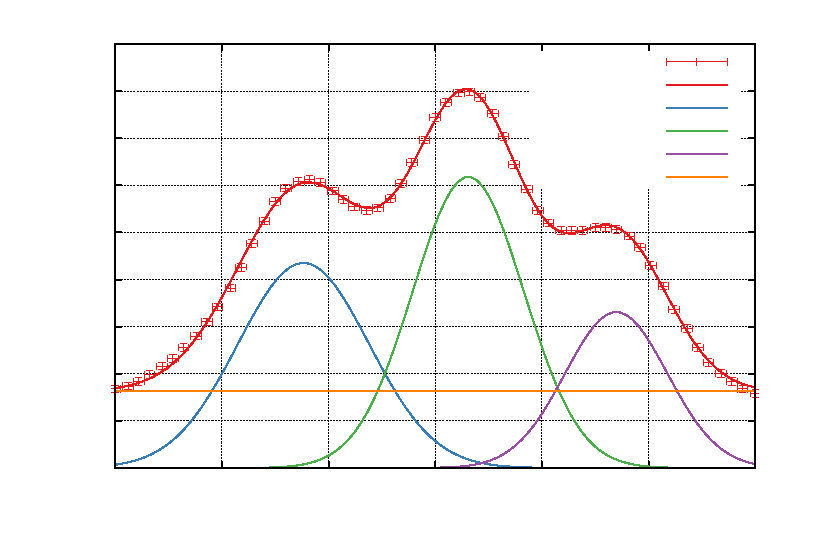
\includegraphics{./plots/zeemann_aufspaltung/b4}}%
    \gplfronttext
  \end{picture}%
\endgroup

	\caption{4 A}
	\label{fig:gauss1}
\end{figure}

\begin{figure}[h]
	\centering
	% GNUPLOT: LaTeX picture with Postscript
\begingroup
  \makeatletter
  \providecommand\color[2][]{%
    \GenericError{(gnuplot) \space\space\space\@spaces}{%
      Package color not loaded in conjunction with
      terminal option `colourtext'%
    }{See the gnuplot documentation for explanation.%
    }{Either use 'blacktext' in gnuplot or load the package
      color.sty in LaTeX.}%
    \renewcommand\color[2][]{}%
  }%
  \providecommand\includegraphics[2][]{%
    \GenericError{(gnuplot) \space\space\space\@spaces}{%
      Package graphicx or graphics not loaded%
    }{See the gnuplot documentation for explanation.%
    }{The gnuplot epslatex terminal needs graphicx.sty or graphics.sty.}%
    \renewcommand\includegraphics[2][]{}%
  }%
  \providecommand\rotatebox[2]{#2}%
  \@ifundefined{ifGPcolor}{%
    \newif\ifGPcolor
    \GPcolortrue
  }{}%
  \@ifundefined{ifGPblacktext}{%
    \newif\ifGPblacktext
    \GPblacktexttrue
  }{}%
  % define a \g@addto@macro without @ in the name:
  \let\gplgaddtomacro\g@addto@macro
  % define empty templates for all commands taking text:
  \gdef\gplbacktext{}%
  \gdef\gplfronttext{}%
  \makeatother
  \ifGPblacktext
    % no textcolor at all
    \def\colorrgb#1{}%
    \def\colorgray#1{}%
  \else
    % gray or color?
    \ifGPcolor
      \def\colorrgb#1{\color[rgb]{#1}}%
      \def\colorgray#1{\color[gray]{#1}}%
      \expandafter\def\csname LTw\endcsname{\color{white}}%
      \expandafter\def\csname LTb\endcsname{\color{black}}%
      \expandafter\def\csname LTa\endcsname{\color{black}}%
      \expandafter\def\csname LT0\endcsname{\color[rgb]{1,0,0}}%
      \expandafter\def\csname LT1\endcsname{\color[rgb]{0,1,0}}%
      \expandafter\def\csname LT2\endcsname{\color[rgb]{0,0,1}}%
      \expandafter\def\csname LT3\endcsname{\color[rgb]{1,0,1}}%
      \expandafter\def\csname LT4\endcsname{\color[rgb]{0,1,1}}%
      \expandafter\def\csname LT5\endcsname{\color[rgb]{1,1,0}}%
      \expandafter\def\csname LT6\endcsname{\color[rgb]{0,0,0}}%
      \expandafter\def\csname LT7\endcsname{\color[rgb]{1,0.3,0}}%
      \expandafter\def\csname LT8\endcsname{\color[rgb]{0.5,0.5,0.5}}%
    \else
      % gray
      \def\colorrgb#1{\color{black}}%
      \def\colorgray#1{\color[gray]{#1}}%
      \expandafter\def\csname LTw\endcsname{\color{white}}%
      \expandafter\def\csname LTb\endcsname{\color{black}}%
      \expandafter\def\csname LTa\endcsname{\color{black}}%
      \expandafter\def\csname LT0\endcsname{\color{black}}%
      \expandafter\def\csname LT1\endcsname{\color{black}}%
      \expandafter\def\csname LT2\endcsname{\color{black}}%
      \expandafter\def\csname LT3\endcsname{\color{black}}%
      \expandafter\def\csname LT4\endcsname{\color{black}}%
      \expandafter\def\csname LT5\endcsname{\color{black}}%
      \expandafter\def\csname LT6\endcsname{\color{black}}%
      \expandafter\def\csname LT7\endcsname{\color{black}}%
      \expandafter\def\csname LT8\endcsname{\color{black}}%
    \fi
  \fi
  \setlength{\unitlength}{0.0500bp}%
  \begin{picture}(7488.00,5040.00)%
    \gplgaddtomacro\gplbacktext{%
      \csname LTb\endcsname%
      \put(814,704){\makebox(0,0)[r]{\strut{} 0}}%
      \csname LTb\endcsname%
      \put(814,1156){\makebox(0,0)[r]{\strut{} 5}}%
      \csname LTb\endcsname%
      \put(814,1609){\makebox(0,0)[r]{\strut{} 10}}%
      \csname LTb\endcsname%
      \put(814,2061){\makebox(0,0)[r]{\strut{} 15}}%
      \csname LTb\endcsname%
      \put(814,2513){\makebox(0,0)[r]{\strut{} 20}}%
      \csname LTb\endcsname%
      \put(814,2966){\makebox(0,0)[r]{\strut{} 25}}%
      \csname LTb\endcsname%
      \put(814,3418){\makebox(0,0)[r]{\strut{} 30}}%
      \csname LTb\endcsname%
      \put(814,3870){\makebox(0,0)[r]{\strut{} 35}}%
      \csname LTb\endcsname%
      \put(814,4323){\makebox(0,0)[r]{\strut{} 40}}%
      \csname LTb\endcsname%
      \put(814,4775){\makebox(0,0)[r]{\strut{} 45}}%
      \csname LTb\endcsname%
      \put(1438,484){\makebox(0,0){\strut{} 0.9}}%
      \csname LTb\endcsname%
      \put(2667,484){\makebox(0,0){\strut{} 0.95}}%
      \csname LTb\endcsname%
      \put(3896,484){\makebox(0,0){\strut{} 1}}%
      \csname LTb\endcsname%
      \put(5125,484){\makebox(0,0){\strut{} 1.05}}%
      \csname LTb\endcsname%
      \put(6354,484){\makebox(0,0){\strut{} 1.1}}%
      \put(176,2739){\rotatebox{-270}{\makebox(0,0){\strut{}Intensität $I$ / \si{\percent}}}}%
      \put(4018,154){\makebox(0,0){\strut{}Winkel $\alpha$ / \si{\degree}}}%
      \put(4018,4665){\makebox(0,0){\strut{}}}%
    }%
    \gplgaddtomacro\gplfronttext{%
      \csname LTb\endcsname%
      \put(6104,4602){\makebox(0,0)[r]{\strut{}Messwerte}}%
      \csname LTb\endcsname%
      \put(6104,4382){\makebox(0,0)[r]{\strut{}$\Sigma$}}%
      \csname LTb\endcsname%
      \put(6104,4162){\makebox(0,0)[r]{\strut{}$\mathcal{G}_1$}}%
      \csname LTb\endcsname%
      \put(6104,3942){\makebox(0,0)[r]{\strut{}$\mathcal{G}_2$}}%
      \csname LTb\endcsname%
      \put(6104,3722){\makebox(0,0)[r]{\strut{}$\mathcal{G}_3$}}%
      \csname LTb\endcsname%
      \put(6104,3502){\makebox(0,0)[r]{\strut{}Untergrund}}%
    }%
    \gplbacktext
    \put(0,0){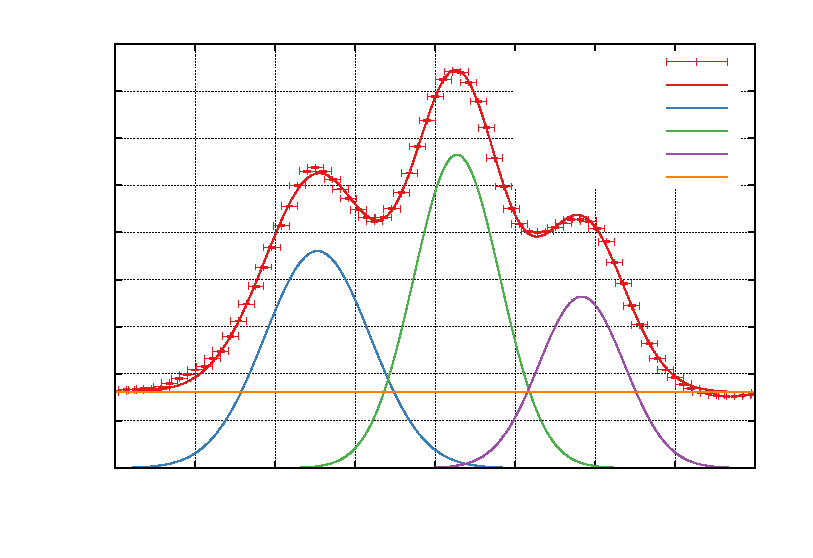
\includegraphics{./plots/zeemann_aufspaltung/b4-5}}%
    \gplfronttext
  \end{picture}%
\endgroup

	\caption{4.5 A}
	\label{fig:gauss2}
\end{figure}

\begin{figure}[h]
	\centering
	% GNUPLOT: LaTeX picture with Postscript
\begingroup
  \makeatletter
  \providecommand\color[2][]{%
    \GenericError{(gnuplot) \space\space\space\@spaces}{%
      Package color not loaded in conjunction with
      terminal option `colourtext'%
    }{See the gnuplot documentation for explanation.%
    }{Either use 'blacktext' in gnuplot or load the package
      color.sty in LaTeX.}%
    \renewcommand\color[2][]{}%
  }%
  \providecommand\includegraphics[2][]{%
    \GenericError{(gnuplot) \space\space\space\@spaces}{%
      Package graphicx or graphics not loaded%
    }{See the gnuplot documentation for explanation.%
    }{The gnuplot epslatex terminal needs graphicx.sty or graphics.sty.}%
    \renewcommand\includegraphics[2][]{}%
  }%
  \providecommand\rotatebox[2]{#2}%
  \@ifundefined{ifGPcolor}{%
    \newif\ifGPcolor
    \GPcolortrue
  }{}%
  \@ifundefined{ifGPblacktext}{%
    \newif\ifGPblacktext
    \GPblacktexttrue
  }{}%
  % define a \g@addto@macro without @ in the name:
  \let\gplgaddtomacro\g@addto@macro
  % define empty templates for all commands taking text:
  \gdef\gplbacktext{}%
  \gdef\gplfronttext{}%
  \makeatother
  \ifGPblacktext
    % no textcolor at all
    \def\colorrgb#1{}%
    \def\colorgray#1{}%
  \else
    % gray or color?
    \ifGPcolor
      \def\colorrgb#1{\color[rgb]{#1}}%
      \def\colorgray#1{\color[gray]{#1}}%
      \expandafter\def\csname LTw\endcsname{\color{white}}%
      \expandafter\def\csname LTb\endcsname{\color{black}}%
      \expandafter\def\csname LTa\endcsname{\color{black}}%
      \expandafter\def\csname LT0\endcsname{\color[rgb]{1,0,0}}%
      \expandafter\def\csname LT1\endcsname{\color[rgb]{0,1,0}}%
      \expandafter\def\csname LT2\endcsname{\color[rgb]{0,0,1}}%
      \expandafter\def\csname LT3\endcsname{\color[rgb]{1,0,1}}%
      \expandafter\def\csname LT4\endcsname{\color[rgb]{0,1,1}}%
      \expandafter\def\csname LT5\endcsname{\color[rgb]{1,1,0}}%
      \expandafter\def\csname LT6\endcsname{\color[rgb]{0,0,0}}%
      \expandafter\def\csname LT7\endcsname{\color[rgb]{1,0.3,0}}%
      \expandafter\def\csname LT8\endcsname{\color[rgb]{0.5,0.5,0.5}}%
    \else
      % gray
      \def\colorrgb#1{\color{black}}%
      \def\colorgray#1{\color[gray]{#1}}%
      \expandafter\def\csname LTw\endcsname{\color{white}}%
      \expandafter\def\csname LTb\endcsname{\color{black}}%
      \expandafter\def\csname LTa\endcsname{\color{black}}%
      \expandafter\def\csname LT0\endcsname{\color{black}}%
      \expandafter\def\csname LT1\endcsname{\color{black}}%
      \expandafter\def\csname LT2\endcsname{\color{black}}%
      \expandafter\def\csname LT3\endcsname{\color{black}}%
      \expandafter\def\csname LT4\endcsname{\color{black}}%
      \expandafter\def\csname LT5\endcsname{\color{black}}%
      \expandafter\def\csname LT6\endcsname{\color{black}}%
      \expandafter\def\csname LT7\endcsname{\color{black}}%
      \expandafter\def\csname LT8\endcsname{\color{black}}%
    \fi
  \fi
  \setlength{\unitlength}{0.0500bp}%
  \begin{picture}(7488.00,5040.00)%
    \gplgaddtomacro\gplbacktext{%
      \csname LTb\endcsname%
      \put(814,704){\makebox(0,0)[r]{\strut{} 0}}%
      \csname LTb\endcsname%
      \put(814,1156){\makebox(0,0)[r]{\strut{} 5}}%
      \csname LTb\endcsname%
      \put(814,1609){\makebox(0,0)[r]{\strut{} 10}}%
      \csname LTb\endcsname%
      \put(814,2061){\makebox(0,0)[r]{\strut{} 15}}%
      \csname LTb\endcsname%
      \put(814,2513){\makebox(0,0)[r]{\strut{} 20}}%
      \csname LTb\endcsname%
      \put(814,2966){\makebox(0,0)[r]{\strut{} 25}}%
      \csname LTb\endcsname%
      \put(814,3418){\makebox(0,0)[r]{\strut{} 30}}%
      \csname LTb\endcsname%
      \put(814,3870){\makebox(0,0)[r]{\strut{} 35}}%
      \csname LTb\endcsname%
      \put(814,4323){\makebox(0,0)[r]{\strut{} 40}}%
      \csname LTb\endcsname%
      \put(814,4775){\makebox(0,0)[r]{\strut{} 45}}%
      \csname LTb\endcsname%
      \put(1655,484){\makebox(0,0){\strut{} 0.9}}%
      \csname LTb\endcsname%
      \put(2837,484){\makebox(0,0){\strut{} 0.95}}%
      \csname LTb\endcsname%
      \put(4019,484){\makebox(0,0){\strut{} 1}}%
      \csname LTb\endcsname%
      \put(5200,484){\makebox(0,0){\strut{} 1.05}}%
      \csname LTb\endcsname%
      \put(6382,484){\makebox(0,0){\strut{} 1.1}}%
      \put(176,2739){\rotatebox{-270}{\makebox(0,0){\strut{}Intensität $I$ / \si{\percent}}}}%
      \put(4018,154){\makebox(0,0){\strut{}Winkel $\alpha$ / \si{\degree}}}%
      \put(4018,4665){\makebox(0,0){\strut{}}}%
    }%
    \gplgaddtomacro\gplfronttext{%
      \csname LTb\endcsname%
      \put(6104,4602){\makebox(0,0)[r]{\strut{}Messwerte}}%
      \csname LTb\endcsname%
      \put(6104,4382){\makebox(0,0)[r]{\strut{}$\Sigma$}}%
      \csname LTb\endcsname%
      \put(6104,4162){\makebox(0,0)[r]{\strut{}$\mathcal{G}_1$}}%
      \csname LTb\endcsname%
      \put(6104,3942){\makebox(0,0)[r]{\strut{}$\mathcal{G}_2$}}%
      \csname LTb\endcsname%
      \put(6104,3722){\makebox(0,0)[r]{\strut{}$\mathcal{G}_3$}}%
      \csname LTb\endcsname%
      \put(6104,3502){\makebox(0,0)[r]{\strut{}Untergrund}}%
    }%
    \gplbacktext
    \put(0,0){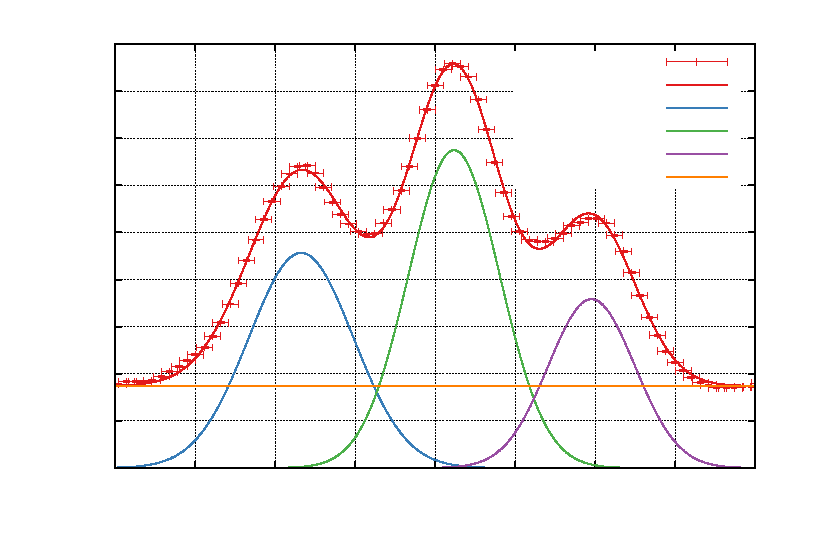
\includegraphics{./plots/zeemann_aufspaltung/b5}}%
    \gplfronttext
  \end{picture}%
\endgroup

	\caption{5A}
	\label{fig:gauss3}
\end{figure}

\begin{figure}[h]
	\centering
	% GNUPLOT: LaTeX picture with Postscript
\begingroup
  \makeatletter
  \providecommand\color[2][]{%
    \GenericError{(gnuplot) \space\space\space\@spaces}{%
      Package color not loaded in conjunction with
      terminal option `colourtext'%
    }{See the gnuplot documentation for explanation.%
    }{Either use 'blacktext' in gnuplot or load the package
      color.sty in LaTeX.}%
    \renewcommand\color[2][]{}%
  }%
  \providecommand\includegraphics[2][]{%
    \GenericError{(gnuplot) \space\space\space\@spaces}{%
      Package graphicx or graphics not loaded%
    }{See the gnuplot documentation for explanation.%
    }{The gnuplot epslatex terminal needs graphicx.sty or graphics.sty.}%
    \renewcommand\includegraphics[2][]{}%
  }%
  \providecommand\rotatebox[2]{#2}%
  \@ifundefined{ifGPcolor}{%
    \newif\ifGPcolor
    \GPcolortrue
  }{}%
  \@ifundefined{ifGPblacktext}{%
    \newif\ifGPblacktext
    \GPblacktexttrue
  }{}%
  % define a \g@addto@macro without @ in the name:
  \let\gplgaddtomacro\g@addto@macro
  % define empty templates for all commands taking text:
  \gdef\gplbacktext{}%
  \gdef\gplfronttext{}%
  \makeatother
  \ifGPblacktext
    % no textcolor at all
    \def\colorrgb#1{}%
    \def\colorgray#1{}%
  \else
    % gray or color?
    \ifGPcolor
      \def\colorrgb#1{\color[rgb]{#1}}%
      \def\colorgray#1{\color[gray]{#1}}%
      \expandafter\def\csname LTw\endcsname{\color{white}}%
      \expandafter\def\csname LTb\endcsname{\color{black}}%
      \expandafter\def\csname LTa\endcsname{\color{black}}%
      \expandafter\def\csname LT0\endcsname{\color[rgb]{1,0,0}}%
      \expandafter\def\csname LT1\endcsname{\color[rgb]{0,1,0}}%
      \expandafter\def\csname LT2\endcsname{\color[rgb]{0,0,1}}%
      \expandafter\def\csname LT3\endcsname{\color[rgb]{1,0,1}}%
      \expandafter\def\csname LT4\endcsname{\color[rgb]{0,1,1}}%
      \expandafter\def\csname LT5\endcsname{\color[rgb]{1,1,0}}%
      \expandafter\def\csname LT6\endcsname{\color[rgb]{0,0,0}}%
      \expandafter\def\csname LT7\endcsname{\color[rgb]{1,0.3,0}}%
      \expandafter\def\csname LT8\endcsname{\color[rgb]{0.5,0.5,0.5}}%
    \else
      % gray
      \def\colorrgb#1{\color{black}}%
      \def\colorgray#1{\color[gray]{#1}}%
      \expandafter\def\csname LTw\endcsname{\color{white}}%
      \expandafter\def\csname LTb\endcsname{\color{black}}%
      \expandafter\def\csname LTa\endcsname{\color{black}}%
      \expandafter\def\csname LT0\endcsname{\color{black}}%
      \expandafter\def\csname LT1\endcsname{\color{black}}%
      \expandafter\def\csname LT2\endcsname{\color{black}}%
      \expandafter\def\csname LT3\endcsname{\color{black}}%
      \expandafter\def\csname LT4\endcsname{\color{black}}%
      \expandafter\def\csname LT5\endcsname{\color{black}}%
      \expandafter\def\csname LT6\endcsname{\color{black}}%
      \expandafter\def\csname LT7\endcsname{\color{black}}%
      \expandafter\def\csname LT8\endcsname{\color{black}}%
    \fi
  \fi
  \setlength{\unitlength}{0.0500bp}%
  \begin{picture}(7486.00,5040.00)%
    \gplgaddtomacro\gplbacktext{%
      \csname LTb\endcsname%
      \put(814,704){\makebox(0,0)[r]{\strut{} 0}}%
      \csname LTb\endcsname%
      \put(814,1156){\makebox(0,0)[r]{\strut{} 5}}%
      \csname LTb\endcsname%
      \put(814,1609){\makebox(0,0)[r]{\strut{} 10}}%
      \csname LTb\endcsname%
      \put(814,2061){\makebox(0,0)[r]{\strut{} 15}}%
      \csname LTb\endcsname%
      \put(814,2513){\makebox(0,0)[r]{\strut{} 20}}%
      \csname LTb\endcsname%
      \put(814,2966){\makebox(0,0)[r]{\strut{} 25}}%
      \csname LTb\endcsname%
      \put(814,3418){\makebox(0,0)[r]{\strut{} 30}}%
      \csname LTb\endcsname%
      \put(814,3870){\makebox(0,0)[r]{\strut{} 35}}%
      \csname LTb\endcsname%
      \put(814,4323){\makebox(0,0)[r]{\strut{} 40}}%
      \csname LTb\endcsname%
      \put(814,4775){\makebox(0,0)[r]{\strut{} 45}}%
      \csname LTb\endcsname%
      \put(946,484){\makebox(0,0){\strut{} 0.8}}%
      \csname LTb\endcsname%
      \put(1714,484){\makebox(0,0){\strut{} 0.85}}%
      \csname LTb\endcsname%
      \put(2482,484){\makebox(0,0){\strut{} 0.9}}%
      \csname LTb\endcsname%
      \put(3250,484){\makebox(0,0){\strut{} 0.95}}%
      \csname LTb\endcsname%
      \put(4018,484){\makebox(0,0){\strut{} 1}}%
      \csname LTb\endcsname%
      \put(4785,484){\makebox(0,0){\strut{} 1.05}}%
      \csname LTb\endcsname%
      \put(5553,484){\makebox(0,0){\strut{} 1.1}}%
      \csname LTb\endcsname%
      \put(6321,484){\makebox(0,0){\strut{} 1.15}}%
      \csname LTb\endcsname%
      \put(7089,484){\makebox(0,0){\strut{} 1.2}}%
      \put(176,2739){\rotatebox{-270}{\makebox(0,0){\strut{}Intensität $I$ / \si{\percent}}}}%
      \put(4017,154){\makebox(0,0){\strut{}Winkel $\alpha$ / \si{\degree}}}%
      \put(4017,4665){\makebox(0,0){\strut{}}}%
    }%
    \gplgaddtomacro\gplfronttext{%
      \csname LTb\endcsname%
      \put(6102,4602){\makebox(0,0)[r]{\strut{}Messwerte}}%
      \csname LTb\endcsname%
      \put(6102,4382){\makebox(0,0)[r]{\strut{}$\Sigma$}}%
      \csname LTb\endcsname%
      \put(6102,4162){\makebox(0,0)[r]{\strut{}$\mathcal{G}_1$}}%
      \csname LTb\endcsname%
      \put(6102,3942){\makebox(0,0)[r]{\strut{}$\mathcal{G}_2$}}%
      \csname LTb\endcsname%
      \put(6102,3722){\makebox(0,0)[r]{\strut{}$\mathcal{G}_3$}}%
      \csname LTb\endcsname%
      \put(6102,3502){\makebox(0,0)[r]{\strut{}Untergrund}}%
    }%
    \gplbacktext
    \put(0,0){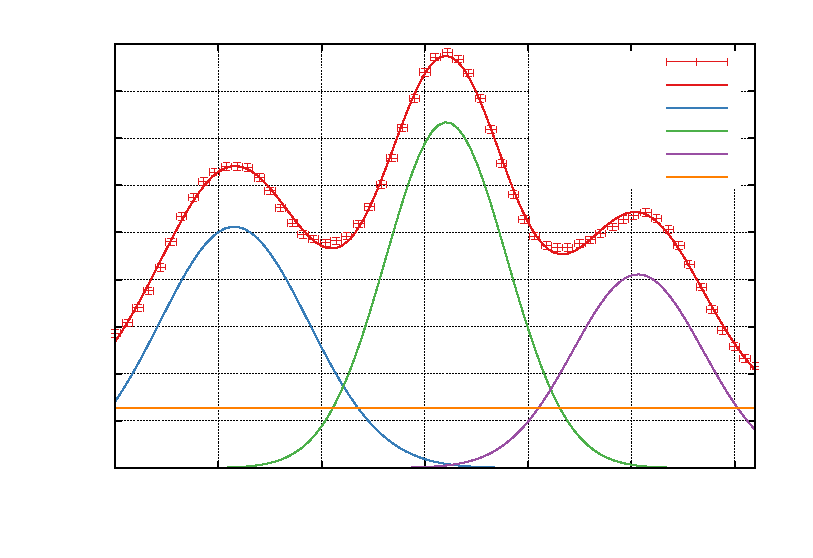
\includegraphics{./plots/zeemann_aufspaltung/b5-5}}%
    \gplfronttext
  \end{picture}%
\endgroup

	\caption{5.5A}
	\label{fig:gauss4}
\end{figure}

\begin{figure}[h]
	\centering
	% GNUPLOT: LaTeX picture with Postscript
\begingroup
  \makeatletter
  \providecommand\color[2][]{%
    \GenericError{(gnuplot) \space\space\space\@spaces}{%
      Package color not loaded in conjunction with
      terminal option `colourtext'%
    }{See the gnuplot documentation for explanation.%
    }{Either use 'blacktext' in gnuplot or load the package
      color.sty in LaTeX.}%
    \renewcommand\color[2][]{}%
  }%
  \providecommand\includegraphics[2][]{%
    \GenericError{(gnuplot) \space\space\space\@spaces}{%
      Package graphicx or graphics not loaded%
    }{See the gnuplot documentation for explanation.%
    }{The gnuplot epslatex terminal needs graphicx.sty or graphics.sty.}%
    \renewcommand\includegraphics[2][]{}%
  }%
  \providecommand\rotatebox[2]{#2}%
  \@ifundefined{ifGPcolor}{%
    \newif\ifGPcolor
    \GPcolortrue
  }{}%
  \@ifundefined{ifGPblacktext}{%
    \newif\ifGPblacktext
    \GPblacktexttrue
  }{}%
  % define a \g@addto@macro without @ in the name:
  \let\gplgaddtomacro\g@addto@macro
  % define empty templates for all commands taking text:
  \gdef\gplbacktext{}%
  \gdef\gplfronttext{}%
  \makeatother
  \ifGPblacktext
    % no textcolor at all
    \def\colorrgb#1{}%
    \def\colorgray#1{}%
  \else
    % gray or color?
    \ifGPcolor
      \def\colorrgb#1{\color[rgb]{#1}}%
      \def\colorgray#1{\color[gray]{#1}}%
      \expandafter\def\csname LTw\endcsname{\color{white}}%
      \expandafter\def\csname LTb\endcsname{\color{black}}%
      \expandafter\def\csname LTa\endcsname{\color{black}}%
      \expandafter\def\csname LT0\endcsname{\color[rgb]{1,0,0}}%
      \expandafter\def\csname LT1\endcsname{\color[rgb]{0,1,0}}%
      \expandafter\def\csname LT2\endcsname{\color[rgb]{0,0,1}}%
      \expandafter\def\csname LT3\endcsname{\color[rgb]{1,0,1}}%
      \expandafter\def\csname LT4\endcsname{\color[rgb]{0,1,1}}%
      \expandafter\def\csname LT5\endcsname{\color[rgb]{1,1,0}}%
      \expandafter\def\csname LT6\endcsname{\color[rgb]{0,0,0}}%
      \expandafter\def\csname LT7\endcsname{\color[rgb]{1,0.3,0}}%
      \expandafter\def\csname LT8\endcsname{\color[rgb]{0.5,0.5,0.5}}%
    \else
      % gray
      \def\colorrgb#1{\color{black}}%
      \def\colorgray#1{\color[gray]{#1}}%
      \expandafter\def\csname LTw\endcsname{\color{white}}%
      \expandafter\def\csname LTb\endcsname{\color{black}}%
      \expandafter\def\csname LTa\endcsname{\color{black}}%
      \expandafter\def\csname LT0\endcsname{\color{black}}%
      \expandafter\def\csname LT1\endcsname{\color{black}}%
      \expandafter\def\csname LT2\endcsname{\color{black}}%
      \expandafter\def\csname LT3\endcsname{\color{black}}%
      \expandafter\def\csname LT4\endcsname{\color{black}}%
      \expandafter\def\csname LT5\endcsname{\color{black}}%
      \expandafter\def\csname LT6\endcsname{\color{black}}%
      \expandafter\def\csname LT7\endcsname{\color{black}}%
      \expandafter\def\csname LT8\endcsname{\color{black}}%
    \fi
  \fi
  \setlength{\unitlength}{0.0500bp}%
  \begin{picture}(7486.00,5040.00)%
    \gplgaddtomacro\gplbacktext{%
      \csname LTb\endcsname%
      \put(814,704){\makebox(0,0)[r]{\strut{} 0}}%
      \csname LTb\endcsname%
      \put(814,1111){\makebox(0,0)[r]{\strut{} 5}}%
      \csname LTb\endcsname%
      \put(814,1518){\makebox(0,0)[r]{\strut{} 10}}%
      \csname LTb\endcsname%
      \put(814,1925){\makebox(0,0)[r]{\strut{} 15}}%
      \csname LTb\endcsname%
      \put(814,2332){\makebox(0,0)[r]{\strut{} 20}}%
      \csname LTb\endcsname%
      \put(814,2740){\makebox(0,0)[r]{\strut{} 25}}%
      \csname LTb\endcsname%
      \put(814,3147){\makebox(0,0)[r]{\strut{} 30}}%
      \csname LTb\endcsname%
      \put(814,3554){\makebox(0,0)[r]{\strut{} 35}}%
      \csname LTb\endcsname%
      \put(814,3961){\makebox(0,0)[r]{\strut{} 40}}%
      \csname LTb\endcsname%
      \put(814,4368){\makebox(0,0)[r]{\strut{} 45}}%
      \csname LTb\endcsname%
      \put(814,4775){\makebox(0,0)[r]{\strut{} 50}}%
      \csname LTb\endcsname%
      \put(946,484){\makebox(0,0){\strut{} 0.8}}%
      \csname LTb\endcsname%
      \put(1714,484){\makebox(0,0){\strut{} 0.85}}%
      \csname LTb\endcsname%
      \put(2482,484){\makebox(0,0){\strut{} 0.9}}%
      \csname LTb\endcsname%
      \put(3250,484){\makebox(0,0){\strut{} 0.95}}%
      \csname LTb\endcsname%
      \put(4018,484){\makebox(0,0){\strut{} 1}}%
      \csname LTb\endcsname%
      \put(4785,484){\makebox(0,0){\strut{} 1.05}}%
      \csname LTb\endcsname%
      \put(5553,484){\makebox(0,0){\strut{} 1.1}}%
      \csname LTb\endcsname%
      \put(6321,484){\makebox(0,0){\strut{} 1.15}}%
      \csname LTb\endcsname%
      \put(7089,484){\makebox(0,0){\strut{} 1.2}}%
      \put(176,2739){\rotatebox{-270}{\makebox(0,0){\strut{}Intensität $I$ / \si{\percent}}}}%
      \put(4017,154){\makebox(0,0){\strut{}Winkel $\alpha$ / \si{\degree}}}%
      \put(4017,4665){\makebox(0,0){\strut{}}}%
    }%
    \gplgaddtomacro\gplfronttext{%
      \csname LTb\endcsname%
      \put(6102,4602){\makebox(0,0)[r]{\strut{}Messwerte}}%
      \csname LTb\endcsname%
      \put(6102,4382){\makebox(0,0)[r]{\strut{}$\Sigma$}}%
      \csname LTb\endcsname%
      \put(6102,4162){\makebox(0,0)[r]{\strut{}$\mathcal{G}_1$}}%
      \csname LTb\endcsname%
      \put(6102,3942){\makebox(0,0)[r]{\strut{}$\mathcal{G}_2$}}%
      \csname LTb\endcsname%
      \put(6102,3722){\makebox(0,0)[r]{\strut{}$\mathcal{G}_3$}}%
      \csname LTb\endcsname%
      \put(6102,3502){\makebox(0,0)[r]{\strut{}Untergrund}}%
    }%
    \gplbacktext
    \put(0,0){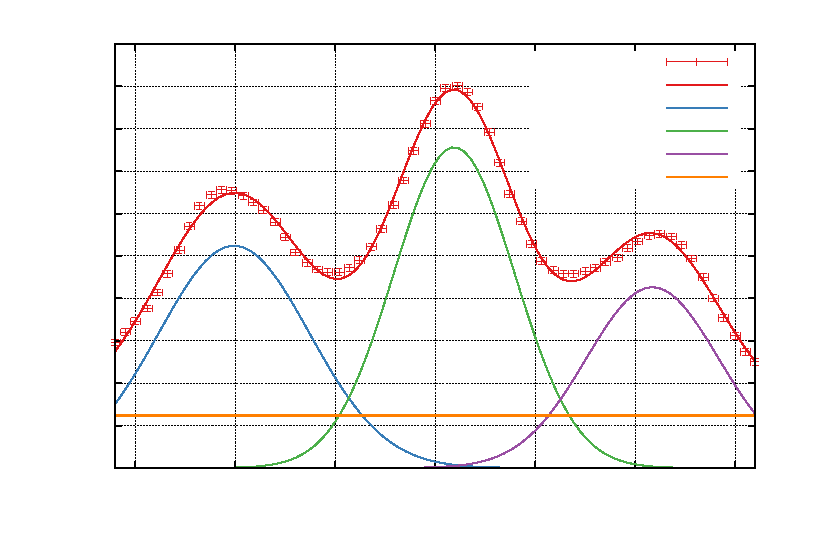
\includegraphics{./plots/zeemann_aufspaltung/b6}}%
    \gplfronttext
  \end{picture}%
\endgroup

	\caption{6A}
	\label{fig:gauss5}
\end{figure}

\begin{figure}[h]
	\centering
	% GNUPLOT: LaTeX picture with Postscript
\begingroup
  \makeatletter
  \providecommand\color[2][]{%
    \GenericError{(gnuplot) \space\space\space\@spaces}{%
      Package color not loaded in conjunction with
      terminal option `colourtext'%
    }{See the gnuplot documentation for explanation.%
    }{Either use 'blacktext' in gnuplot or load the package
      color.sty in LaTeX.}%
    \renewcommand\color[2][]{}%
  }%
  \providecommand\includegraphics[2][]{%
    \GenericError{(gnuplot) \space\space\space\@spaces}{%
      Package graphicx or graphics not loaded%
    }{See the gnuplot documentation for explanation.%
    }{The gnuplot epslatex terminal needs graphicx.sty or graphics.sty.}%
    \renewcommand\includegraphics[2][]{}%
  }%
  \providecommand\rotatebox[2]{#2}%
  \@ifundefined{ifGPcolor}{%
    \newif\ifGPcolor
    \GPcolortrue
  }{}%
  \@ifundefined{ifGPblacktext}{%
    \newif\ifGPblacktext
    \GPblacktexttrue
  }{}%
  % define a \g@addto@macro without @ in the name:
  \let\gplgaddtomacro\g@addto@macro
  % define empty templates for all commands taking text:
  \gdef\gplbacktext{}%
  \gdef\gplfronttext{}%
  \makeatother
  \ifGPblacktext
    % no textcolor at all
    \def\colorrgb#1{}%
    \def\colorgray#1{}%
  \else
    % gray or color?
    \ifGPcolor
      \def\colorrgb#1{\color[rgb]{#1}}%
      \def\colorgray#1{\color[gray]{#1}}%
      \expandafter\def\csname LTw\endcsname{\color{white}}%
      \expandafter\def\csname LTb\endcsname{\color{black}}%
      \expandafter\def\csname LTa\endcsname{\color{black}}%
      \expandafter\def\csname LT0\endcsname{\color[rgb]{1,0,0}}%
      \expandafter\def\csname LT1\endcsname{\color[rgb]{0,1,0}}%
      \expandafter\def\csname LT2\endcsname{\color[rgb]{0,0,1}}%
      \expandafter\def\csname LT3\endcsname{\color[rgb]{1,0,1}}%
      \expandafter\def\csname LT4\endcsname{\color[rgb]{0,1,1}}%
      \expandafter\def\csname LT5\endcsname{\color[rgb]{1,1,0}}%
      \expandafter\def\csname LT6\endcsname{\color[rgb]{0,0,0}}%
      \expandafter\def\csname LT7\endcsname{\color[rgb]{1,0.3,0}}%
      \expandafter\def\csname LT8\endcsname{\color[rgb]{0.5,0.5,0.5}}%
    \else
      % gray
      \def\colorrgb#1{\color{black}}%
      \def\colorgray#1{\color[gray]{#1}}%
      \expandafter\def\csname LTw\endcsname{\color{white}}%
      \expandafter\def\csname LTb\endcsname{\color{black}}%
      \expandafter\def\csname LTa\endcsname{\color{black}}%
      \expandafter\def\csname LT0\endcsname{\color{black}}%
      \expandafter\def\csname LT1\endcsname{\color{black}}%
      \expandafter\def\csname LT2\endcsname{\color{black}}%
      \expandafter\def\csname LT3\endcsname{\color{black}}%
      \expandafter\def\csname LT4\endcsname{\color{black}}%
      \expandafter\def\csname LT5\endcsname{\color{black}}%
      \expandafter\def\csname LT6\endcsname{\color{black}}%
      \expandafter\def\csname LT7\endcsname{\color{black}}%
      \expandafter\def\csname LT8\endcsname{\color{black}}%
    \fi
  \fi
  \setlength{\unitlength}{0.0500bp}%
  \begin{picture}(7488.00,5040.00)%
    \gplgaddtomacro\gplbacktext{%
      \csname LTb\endcsname%
      \put(814,704){\makebox(0,0)[r]{\strut{} 0}}%
      \csname LTb\endcsname%
      \put(814,1111){\makebox(0,0)[r]{\strut{} 5}}%
      \csname LTb\endcsname%
      \put(814,1518){\makebox(0,0)[r]{\strut{} 10}}%
      \csname LTb\endcsname%
      \put(814,1925){\makebox(0,0)[r]{\strut{} 15}}%
      \csname LTb\endcsname%
      \put(814,2332){\makebox(0,0)[r]{\strut{} 20}}%
      \csname LTb\endcsname%
      \put(814,2740){\makebox(0,0)[r]{\strut{} 25}}%
      \csname LTb\endcsname%
      \put(814,3147){\makebox(0,0)[r]{\strut{} 30}}%
      \csname LTb\endcsname%
      \put(814,3554){\makebox(0,0)[r]{\strut{} 35}}%
      \csname LTb\endcsname%
      \put(814,3961){\makebox(0,0)[r]{\strut{} 40}}%
      \csname LTb\endcsname%
      \put(814,4368){\makebox(0,0)[r]{\strut{} 45}}%
      \csname LTb\endcsname%
      \put(814,4775){\makebox(0,0)[r]{\strut{} 50}}%
      \csname LTb\endcsname%
      \put(1307,484){\makebox(0,0){\strut{} 0.85}}%
      \csname LTb\endcsname%
      \put(2211,484){\makebox(0,0){\strut{} 0.9}}%
      \csname LTb\endcsname%
      \put(3115,484){\makebox(0,0){\strut{} 0.95}}%
      \csname LTb\endcsname%
      \put(4019,484){\makebox(0,0){\strut{} 1}}%
      \csname LTb\endcsname%
      \put(4922,484){\makebox(0,0){\strut{} 1.05}}%
      \csname LTb\endcsname%
      \put(5826,484){\makebox(0,0){\strut{} 1.1}}%
      \csname LTb\endcsname%
      \put(6730,484){\makebox(0,0){\strut{} 1.15}}%
      \put(176,2739){\rotatebox{-270}{\makebox(0,0){\strut{}Intensität $I$ / \si{\percent}}}}%
      \put(4018,154){\makebox(0,0){\strut{}Winkel $\alpha$ / \si{\degree}}}%
      \put(4018,4665){\makebox(0,0){\strut{}}}%
    }%
    \gplgaddtomacro\gplfronttext{%
      \csname LTb\endcsname%
      \put(6104,4602){\makebox(0,0)[r]{\strut{}Messwerte}}%
      \csname LTb\endcsname%
      \put(6104,4382){\makebox(0,0)[r]{\strut{}$\Sigma$}}%
      \csname LTb\endcsname%
      \put(6104,4162){\makebox(0,0)[r]{\strut{}$\mathcal{G}_1$}}%
      \csname LTb\endcsname%
      \put(6104,3942){\makebox(0,0)[r]{\strut{}$\mathcal{G}_2$}}%
      \csname LTb\endcsname%
      \put(6104,3722){\makebox(0,0)[r]{\strut{}$\mathcal{G}_3$}}%
      \csname LTb\endcsname%
      \put(6104,3502){\makebox(0,0)[r]{\strut{}$d$}}%
    }%
    \gplbacktext
    \put(0,0){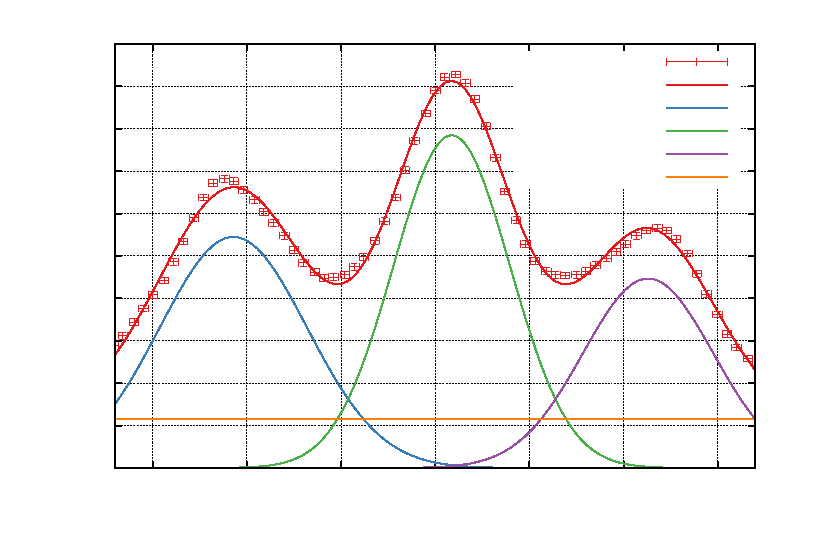
\includegraphics{./plots/zeemann_aufspaltung/b6-5}}%
    \gplfronttext
  \end{picture}%
\endgroup

	\caption{6.5A}
	\label{fig:gauss6}
\end{figure}

\begin{figure}[h]
	\centering
	% GNUPLOT: LaTeX picture with Postscript
\begingroup
  \makeatletter
  \providecommand\color[2][]{%
    \GenericError{(gnuplot) \space\space\space\@spaces}{%
      Package color not loaded in conjunction with
      terminal option `colourtext'%
    }{See the gnuplot documentation for explanation.%
    }{Either use 'blacktext' in gnuplot or load the package
      color.sty in LaTeX.}%
    \renewcommand\color[2][]{}%
  }%
  \providecommand\includegraphics[2][]{%
    \GenericError{(gnuplot) \space\space\space\@spaces}{%
      Package graphicx or graphics not loaded%
    }{See the gnuplot documentation for explanation.%
    }{The gnuplot epslatex terminal needs graphicx.sty or graphics.sty.}%
    \renewcommand\includegraphics[2][]{}%
  }%
  \providecommand\rotatebox[2]{#2}%
  \@ifundefined{ifGPcolor}{%
    \newif\ifGPcolor
    \GPcolortrue
  }{}%
  \@ifundefined{ifGPblacktext}{%
    \newif\ifGPblacktext
    \GPblacktexttrue
  }{}%
  % define a \g@addto@macro without @ in the name:
  \let\gplgaddtomacro\g@addto@macro
  % define empty templates for all commands taking text:
  \gdef\gplbacktext{}%
  \gdef\gplfronttext{}%
  \makeatother
  \ifGPblacktext
    % no textcolor at all
    \def\colorrgb#1{}%
    \def\colorgray#1{}%
  \else
    % gray or color?
    \ifGPcolor
      \def\colorrgb#1{\color[rgb]{#1}}%
      \def\colorgray#1{\color[gray]{#1}}%
      \expandafter\def\csname LTw\endcsname{\color{white}}%
      \expandafter\def\csname LTb\endcsname{\color{black}}%
      \expandafter\def\csname LTa\endcsname{\color{black}}%
      \expandafter\def\csname LT0\endcsname{\color[rgb]{1,0,0}}%
      \expandafter\def\csname LT1\endcsname{\color[rgb]{0,1,0}}%
      \expandafter\def\csname LT2\endcsname{\color[rgb]{0,0,1}}%
      \expandafter\def\csname LT3\endcsname{\color[rgb]{1,0,1}}%
      \expandafter\def\csname LT4\endcsname{\color[rgb]{0,1,1}}%
      \expandafter\def\csname LT5\endcsname{\color[rgb]{1,1,0}}%
      \expandafter\def\csname LT6\endcsname{\color[rgb]{0,0,0}}%
      \expandafter\def\csname LT7\endcsname{\color[rgb]{1,0.3,0}}%
      \expandafter\def\csname LT8\endcsname{\color[rgb]{0.5,0.5,0.5}}%
    \else
      % gray
      \def\colorrgb#1{\color{black}}%
      \def\colorgray#1{\color[gray]{#1}}%
      \expandafter\def\csname LTw\endcsname{\color{white}}%
      \expandafter\def\csname LTb\endcsname{\color{black}}%
      \expandafter\def\csname LTa\endcsname{\color{black}}%
      \expandafter\def\csname LT0\endcsname{\color{black}}%
      \expandafter\def\csname LT1\endcsname{\color{black}}%
      \expandafter\def\csname LT2\endcsname{\color{black}}%
      \expandafter\def\csname LT3\endcsname{\color{black}}%
      \expandafter\def\csname LT4\endcsname{\color{black}}%
      \expandafter\def\csname LT5\endcsname{\color{black}}%
      \expandafter\def\csname LT6\endcsname{\color{black}}%
      \expandafter\def\csname LT7\endcsname{\color{black}}%
      \expandafter\def\csname LT8\endcsname{\color{black}}%
    \fi
  \fi
  \setlength{\unitlength}{0.0500bp}%
  \begin{picture}(7486.00,5040.00)%
    \gplgaddtomacro\gplbacktext{%
      \csname LTb\endcsname%
      \put(814,704){\makebox(0,0)[r]{\strut{} 0}}%
      \csname LTb\endcsname%
      \put(814,1111){\makebox(0,0)[r]{\strut{} 5}}%
      \csname LTb\endcsname%
      \put(814,1518){\makebox(0,0)[r]{\strut{} 10}}%
      \csname LTb\endcsname%
      \put(814,1925){\makebox(0,0)[r]{\strut{} 15}}%
      \csname LTb\endcsname%
      \put(814,2332){\makebox(0,0)[r]{\strut{} 20}}%
      \csname LTb\endcsname%
      \put(814,2740){\makebox(0,0)[r]{\strut{} 25}}%
      \csname LTb\endcsname%
      \put(814,3147){\makebox(0,0)[r]{\strut{} 30}}%
      \csname LTb\endcsname%
      \put(814,3554){\makebox(0,0)[r]{\strut{} 35}}%
      \csname LTb\endcsname%
      \put(814,3961){\makebox(0,0)[r]{\strut{} 40}}%
      \csname LTb\endcsname%
      \put(814,4368){\makebox(0,0)[r]{\strut{} 45}}%
      \csname LTb\endcsname%
      \put(814,4775){\makebox(0,0)[r]{\strut{} 50}}%
      \csname LTb\endcsname%
      \put(946,484){\makebox(0,0){\strut{} 0.8}}%
      \csname LTb\endcsname%
      \put(1714,484){\makebox(0,0){\strut{} 0.85}}%
      \csname LTb\endcsname%
      \put(2482,484){\makebox(0,0){\strut{} 0.9}}%
      \csname LTb\endcsname%
      \put(3250,484){\makebox(0,0){\strut{} 0.95}}%
      \csname LTb\endcsname%
      \put(4018,484){\makebox(0,0){\strut{} 1}}%
      \csname LTb\endcsname%
      \put(4785,484){\makebox(0,0){\strut{} 1.05}}%
      \csname LTb\endcsname%
      \put(5553,484){\makebox(0,0){\strut{} 1.1}}%
      \csname LTb\endcsname%
      \put(6321,484){\makebox(0,0){\strut{} 1.15}}%
      \csname LTb\endcsname%
      \put(7089,484){\makebox(0,0){\strut{} 1.2}}%
      \put(176,2739){\rotatebox{-270}{\makebox(0,0){\strut{}Intensität $I$ / \si{\percent}}}}%
      \put(4017,154){\makebox(0,0){\strut{}Winkel $\alpha$ / \si{\degree}}}%
      \put(4017,4665){\makebox(0,0){\strut{}}}%
    }%
    \gplgaddtomacro\gplfronttext{%
      \csname LTb\endcsname%
      \put(6102,4602){\makebox(0,0)[r]{\strut{}Messwerte}}%
      \csname LTb\endcsname%
      \put(6102,4382){\makebox(0,0)[r]{\strut{}$\Sigma$}}%
      \csname LTb\endcsname%
      \put(6102,4162){\makebox(0,0)[r]{\strut{}$\mathcal{G}_1$}}%
      \csname LTb\endcsname%
      \put(6102,3942){\makebox(0,0)[r]{\strut{}$\mathcal{G}_2$}}%
      \csname LTb\endcsname%
      \put(6102,3722){\makebox(0,0)[r]{\strut{}$\mathcal{G}_3$}}%
      \csname LTb\endcsname%
      \put(6102,3502){\makebox(0,0)[r]{\strut{}Untergrund}}%
    }%
    \gplbacktext
    \put(0,0){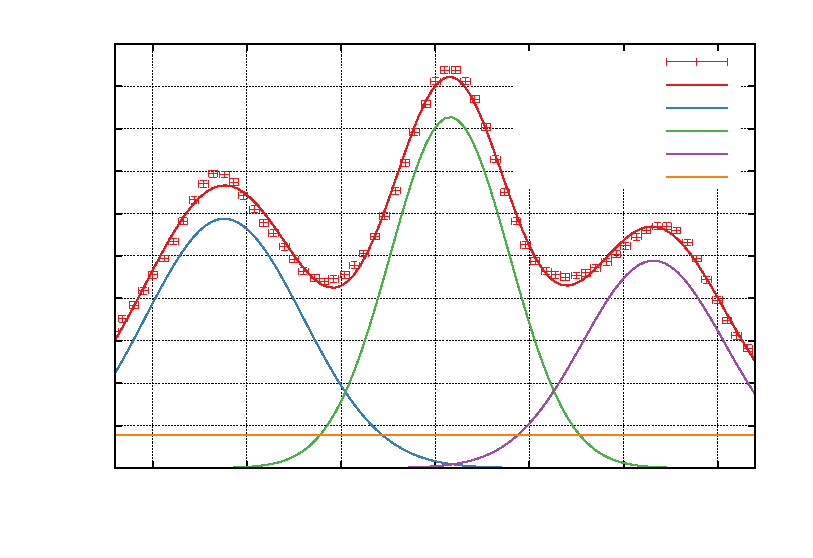
\includegraphics{./plots/zeemann_aufspaltung/b7}}%
    \gplfronttext
  \end{picture}%
\endgroup

	\caption{7 A}
	\label{fig:gauss7}
\end{figure}

\begin{figure}[h]
	\centering
	% GNUPLOT: LaTeX picture with Postscript
\begingroup
  \makeatletter
  \providecommand\color[2][]{%
    \GenericError{(gnuplot) \space\space\space\@spaces}{%
      Package color not loaded in conjunction with
      terminal option `colourtext'%
    }{See the gnuplot documentation for explanation.%
    }{Either use 'blacktext' in gnuplot or load the package
      color.sty in LaTeX.}%
    \renewcommand\color[2][]{}%
  }%
  \providecommand\includegraphics[2][]{%
    \GenericError{(gnuplot) \space\space\space\@spaces}{%
      Package graphicx or graphics not loaded%
    }{See the gnuplot documentation for explanation.%
    }{The gnuplot epslatex terminal needs graphicx.sty or graphics.sty.}%
    \renewcommand\includegraphics[2][]{}%
  }%
  \providecommand\rotatebox[2]{#2}%
  \@ifundefined{ifGPcolor}{%
    \newif\ifGPcolor
    \GPcolortrue
  }{}%
  \@ifundefined{ifGPblacktext}{%
    \newif\ifGPblacktext
    \GPblacktexttrue
  }{}%
  % define a \g@addto@macro without @ in the name:
  \let\gplgaddtomacro\g@addto@macro
  % define empty templates for all commands taking text:
  \gdef\gplbacktext{}%
  \gdef\gplfronttext{}%
  \makeatother
  \ifGPblacktext
    % no textcolor at all
    \def\colorrgb#1{}%
    \def\colorgray#1{}%
  \else
    % gray or color?
    \ifGPcolor
      \def\colorrgb#1{\color[rgb]{#1}}%
      \def\colorgray#1{\color[gray]{#1}}%
      \expandafter\def\csname LTw\endcsname{\color{white}}%
      \expandafter\def\csname LTb\endcsname{\color{black}}%
      \expandafter\def\csname LTa\endcsname{\color{black}}%
      \expandafter\def\csname LT0\endcsname{\color[rgb]{1,0,0}}%
      \expandafter\def\csname LT1\endcsname{\color[rgb]{0,1,0}}%
      \expandafter\def\csname LT2\endcsname{\color[rgb]{0,0,1}}%
      \expandafter\def\csname LT3\endcsname{\color[rgb]{1,0,1}}%
      \expandafter\def\csname LT4\endcsname{\color[rgb]{0,1,1}}%
      \expandafter\def\csname LT5\endcsname{\color[rgb]{1,1,0}}%
      \expandafter\def\csname LT6\endcsname{\color[rgb]{0,0,0}}%
      \expandafter\def\csname LT7\endcsname{\color[rgb]{1,0.3,0}}%
      \expandafter\def\csname LT8\endcsname{\color[rgb]{0.5,0.5,0.5}}%
    \else
      % gray
      \def\colorrgb#1{\color{black}}%
      \def\colorgray#1{\color[gray]{#1}}%
      \expandafter\def\csname LTw\endcsname{\color{white}}%
      \expandafter\def\csname LTb\endcsname{\color{black}}%
      \expandafter\def\csname LTa\endcsname{\color{black}}%
      \expandafter\def\csname LT0\endcsname{\color{black}}%
      \expandafter\def\csname LT1\endcsname{\color{black}}%
      \expandafter\def\csname LT2\endcsname{\color{black}}%
      \expandafter\def\csname LT3\endcsname{\color{black}}%
      \expandafter\def\csname LT4\endcsname{\color{black}}%
      \expandafter\def\csname LT5\endcsname{\color{black}}%
      \expandafter\def\csname LT6\endcsname{\color{black}}%
      \expandafter\def\csname LT7\endcsname{\color{black}}%
      \expandafter\def\csname LT8\endcsname{\color{black}}%
    \fi
  \fi
  \setlength{\unitlength}{0.0500bp}%
  \begin{picture}(7488.00,5040.00)%
    \gplgaddtomacro\gplbacktext{%
      \csname LTb\endcsname%
      \put(814,704){\makebox(0,0)[r]{\strut{} 0}}%
      \csname LTb\endcsname%
      \put(814,1111){\makebox(0,0)[r]{\strut{} 5}}%
      \csname LTb\endcsname%
      \put(814,1518){\makebox(0,0)[r]{\strut{} 10}}%
      \csname LTb\endcsname%
      \put(814,1925){\makebox(0,0)[r]{\strut{} 15}}%
      \csname LTb\endcsname%
      \put(814,2332){\makebox(0,0)[r]{\strut{} 20}}%
      \csname LTb\endcsname%
      \put(814,2740){\makebox(0,0)[r]{\strut{} 25}}%
      \csname LTb\endcsname%
      \put(814,3147){\makebox(0,0)[r]{\strut{} 30}}%
      \csname LTb\endcsname%
      \put(814,3554){\makebox(0,0)[r]{\strut{} 35}}%
      \csname LTb\endcsname%
      \put(814,3961){\makebox(0,0)[r]{\strut{} 40}}%
      \csname LTb\endcsname%
      \put(814,4368){\makebox(0,0)[r]{\strut{} 45}}%
      \csname LTb\endcsname%
      \put(814,4775){\makebox(0,0)[r]{\strut{} 50}}%
      \csname LTb\endcsname%
      \put(1307,484){\makebox(0,0){\strut{} 0.85}}%
      \csname LTb\endcsname%
      \put(2211,484){\makebox(0,0){\strut{} 0.9}}%
      \csname LTb\endcsname%
      \put(3115,484){\makebox(0,0){\strut{} 0.95}}%
      \csname LTb\endcsname%
      \put(4019,484){\makebox(0,0){\strut{} 1}}%
      \csname LTb\endcsname%
      \put(4922,484){\makebox(0,0){\strut{} 1.05}}%
      \csname LTb\endcsname%
      \put(5826,484){\makebox(0,0){\strut{} 1.1}}%
      \csname LTb\endcsname%
      \put(6730,484){\makebox(0,0){\strut{} 1.15}}%
      \put(176,2739){\rotatebox{-270}{\makebox(0,0){\strut{}Intensität $I$ / \si{\percent}}}}%
      \put(4018,154){\makebox(0,0){\strut{}Winkel $\alpha$ / \si{\degree}}}%
      \put(4018,4665){\makebox(0,0){\strut{}}}%
    }%
    \gplgaddtomacro\gplfronttext{%
      \csname LTb\endcsname%
      \put(6104,4602){\makebox(0,0)[r]{\strut{}Messwerte}}%
      \csname LTb\endcsname%
      \put(6104,4382){\makebox(0,0)[r]{\strut{}$\Sigma$}}%
      \csname LTb\endcsname%
      \put(6104,4162){\makebox(0,0)[r]{\strut{}$\mathcal{G}_1$}}%
      \csname LTb\endcsname%
      \put(6104,3942){\makebox(0,0)[r]{\strut{}$\mathcal{G}_2$}}%
      \csname LTb\endcsname%
      \put(6104,3722){\makebox(0,0)[r]{\strut{}$\mathcal{G}_3$}}%
      \csname LTb\endcsname%
      \put(6104,3502){\makebox(0,0)[r]{\strut{}$d$}}%
    }%
    \gplbacktext
    \put(0,0){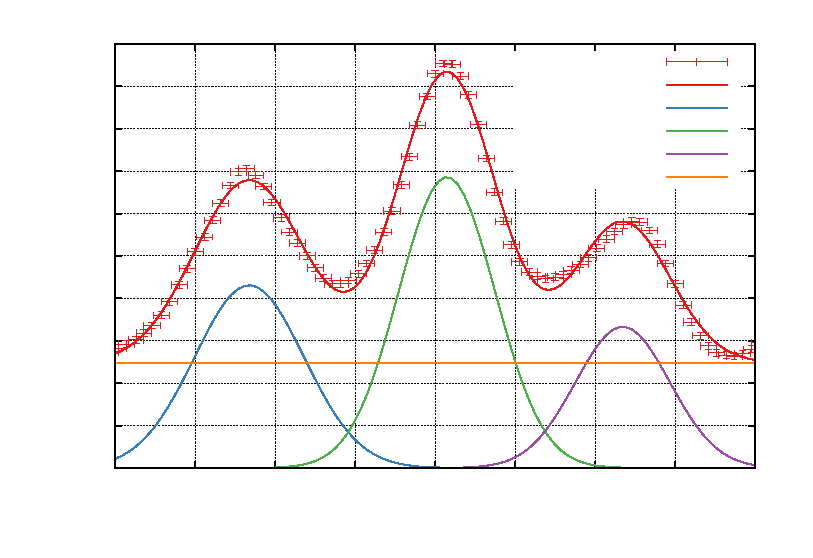
\includegraphics{./plots/zeemann_aufspaltung/b7-5}}%
    \gplfronttext
  \end{picture}%
\endgroup

	\caption{7.5A}
	\label{fig:gauss8}
\end{figure}

\begin{figure}[h]
	\centering
	% GNUPLOT: LaTeX picture with Postscript
\begingroup
  \makeatletter
  \providecommand\color[2][]{%
    \GenericError{(gnuplot) \space\space\space\@spaces}{%
      Package color not loaded in conjunction with
      terminal option `colourtext'%
    }{See the gnuplot documentation for explanation.%
    }{Either use 'blacktext' in gnuplot or load the package
      color.sty in LaTeX.}%
    \renewcommand\color[2][]{}%
  }%
  \providecommand\includegraphics[2][]{%
    \GenericError{(gnuplot) \space\space\space\@spaces}{%
      Package graphicx or graphics not loaded%
    }{See the gnuplot documentation for explanation.%
    }{The gnuplot epslatex terminal needs graphicx.sty or graphics.sty.}%
    \renewcommand\includegraphics[2][]{}%
  }%
  \providecommand\rotatebox[2]{#2}%
  \@ifundefined{ifGPcolor}{%
    \newif\ifGPcolor
    \GPcolortrue
  }{}%
  \@ifundefined{ifGPblacktext}{%
    \newif\ifGPblacktext
    \GPblacktexttrue
  }{}%
  % define a \g@addto@macro without @ in the name:
  \let\gplgaddtomacro\g@addto@macro
  % define empty templates for all commands taking text:
  \gdef\gplbacktext{}%
  \gdef\gplfronttext{}%
  \makeatother
  \ifGPblacktext
    % no textcolor at all
    \def\colorrgb#1{}%
    \def\colorgray#1{}%
  \else
    % gray or color?
    \ifGPcolor
      \def\colorrgb#1{\color[rgb]{#1}}%
      \def\colorgray#1{\color[gray]{#1}}%
      \expandafter\def\csname LTw\endcsname{\color{white}}%
      \expandafter\def\csname LTb\endcsname{\color{black}}%
      \expandafter\def\csname LTa\endcsname{\color{black}}%
      \expandafter\def\csname LT0\endcsname{\color[rgb]{1,0,0}}%
      \expandafter\def\csname LT1\endcsname{\color[rgb]{0,1,0}}%
      \expandafter\def\csname LT2\endcsname{\color[rgb]{0,0,1}}%
      \expandafter\def\csname LT3\endcsname{\color[rgb]{1,0,1}}%
      \expandafter\def\csname LT4\endcsname{\color[rgb]{0,1,1}}%
      \expandafter\def\csname LT5\endcsname{\color[rgb]{1,1,0}}%
      \expandafter\def\csname LT6\endcsname{\color[rgb]{0,0,0}}%
      \expandafter\def\csname LT7\endcsname{\color[rgb]{1,0.3,0}}%
      \expandafter\def\csname LT8\endcsname{\color[rgb]{0.5,0.5,0.5}}%
    \else
      % gray
      \def\colorrgb#1{\color{black}}%
      \def\colorgray#1{\color[gray]{#1}}%
      \expandafter\def\csname LTw\endcsname{\color{white}}%
      \expandafter\def\csname LTb\endcsname{\color{black}}%
      \expandafter\def\csname LTa\endcsname{\color{black}}%
      \expandafter\def\csname LT0\endcsname{\color{black}}%
      \expandafter\def\csname LT1\endcsname{\color{black}}%
      \expandafter\def\csname LT2\endcsname{\color{black}}%
      \expandafter\def\csname LT3\endcsname{\color{black}}%
      \expandafter\def\csname LT4\endcsname{\color{black}}%
      \expandafter\def\csname LT5\endcsname{\color{black}}%
      \expandafter\def\csname LT6\endcsname{\color{black}}%
      \expandafter\def\csname LT7\endcsname{\color{black}}%
      \expandafter\def\csname LT8\endcsname{\color{black}}%
    \fi
  \fi
  \setlength{\unitlength}{0.0500bp}%
  \begin{picture}(7486.00,5040.00)%
    \gplgaddtomacro\gplbacktext{%
      \csname LTb\endcsname%
      \put(814,704){\makebox(0,0)[r]{\strut{} 0}}%
      \csname LTb\endcsname%
      \put(814,1111){\makebox(0,0)[r]{\strut{} 5}}%
      \csname LTb\endcsname%
      \put(814,1518){\makebox(0,0)[r]{\strut{} 10}}%
      \csname LTb\endcsname%
      \put(814,1925){\makebox(0,0)[r]{\strut{} 15}}%
      \csname LTb\endcsname%
      \put(814,2332){\makebox(0,0)[r]{\strut{} 20}}%
      \csname LTb\endcsname%
      \put(814,2740){\makebox(0,0)[r]{\strut{} 25}}%
      \csname LTb\endcsname%
      \put(814,3147){\makebox(0,0)[r]{\strut{} 30}}%
      \csname LTb\endcsname%
      \put(814,3554){\makebox(0,0)[r]{\strut{} 35}}%
      \csname LTb\endcsname%
      \put(814,3961){\makebox(0,0)[r]{\strut{} 40}}%
      \csname LTb\endcsname%
      \put(814,4368){\makebox(0,0)[r]{\strut{} 45}}%
      \csname LTb\endcsname%
      \put(814,4775){\makebox(0,0)[r]{\strut{} 50}}%
      \csname LTb\endcsname%
      \put(946,484){\makebox(0,0){\strut{} 0.8}}%
      \csname LTb\endcsname%
      \put(1714,484){\makebox(0,0){\strut{} 0.85}}%
      \csname LTb\endcsname%
      \put(2482,484){\makebox(0,0){\strut{} 0.9}}%
      \csname LTb\endcsname%
      \put(3250,484){\makebox(0,0){\strut{} 0.95}}%
      \csname LTb\endcsname%
      \put(4018,484){\makebox(0,0){\strut{} 1}}%
      \csname LTb\endcsname%
      \put(4785,484){\makebox(0,0){\strut{} 1.05}}%
      \csname LTb\endcsname%
      \put(5553,484){\makebox(0,0){\strut{} 1.1}}%
      \csname LTb\endcsname%
      \put(6321,484){\makebox(0,0){\strut{} 1.15}}%
      \csname LTb\endcsname%
      \put(7089,484){\makebox(0,0){\strut{} 1.2}}%
      \put(176,2739){\rotatebox{-270}{\makebox(0,0){\strut{}Intensität $I$ / \si{\percent}}}}%
      \put(4017,154){\makebox(0,0){\strut{}Winkel $\alpha$ / \si{\degree}}}%
      \put(4017,4665){\makebox(0,0){\strut{}}}%
    }%
    \gplgaddtomacro\gplfronttext{%
      \csname LTb\endcsname%
      \put(6102,4602){\makebox(0,0)[r]{\strut{}Messwerte}}%
      \csname LTb\endcsname%
      \put(6102,4382){\makebox(0,0)[r]{\strut{}$\Sigma$}}%
      \csname LTb\endcsname%
      \put(6102,4162){\makebox(0,0)[r]{\strut{}$\mathcal{G}_1$}}%
      \csname LTb\endcsname%
      \put(6102,3942){\makebox(0,0)[r]{\strut{}$\mathcal{G}_2$}}%
      \csname LTb\endcsname%
      \put(6102,3722){\makebox(0,0)[r]{\strut{}$\mathcal{G}_3$}}%
      \csname LTb\endcsname%
      \put(6102,3502){\makebox(0,0)[r]{\strut{}Untergrund}}%
    }%
    \gplbacktext
    \put(0,0){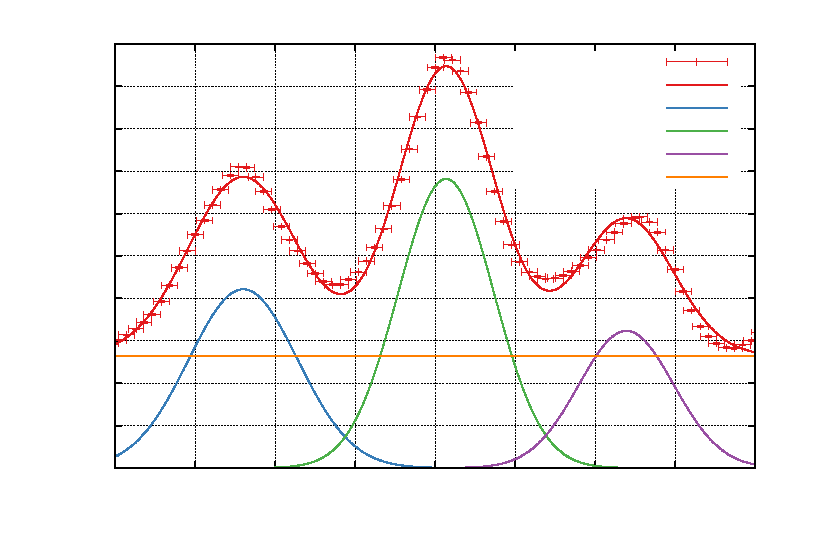
\includegraphics{./plots/zeemann_aufspaltung/b8}}%
    \gplfronttext
  \end{picture}%
\endgroup

	\caption{8A}
	\label{fig:gauss9}
\end{figure}

\begin{figure}[h]
	\centering
	% GNUPLOT: LaTeX picture with Postscript
\begingroup
  \makeatletter
  \providecommand\color[2][]{%
    \GenericError{(gnuplot) \space\space\space\@spaces}{%
      Package color not loaded in conjunction with
      terminal option `colourtext'%
    }{See the gnuplot documentation for explanation.%
    }{Either use 'blacktext' in gnuplot or load the package
      color.sty in LaTeX.}%
    \renewcommand\color[2][]{}%
  }%
  \providecommand\includegraphics[2][]{%
    \GenericError{(gnuplot) \space\space\space\@spaces}{%
      Package graphicx or graphics not loaded%
    }{See the gnuplot documentation for explanation.%
    }{The gnuplot epslatex terminal needs graphicx.sty or graphics.sty.}%
    \renewcommand\includegraphics[2][]{}%
  }%
  \providecommand\rotatebox[2]{#2}%
  \@ifundefined{ifGPcolor}{%
    \newif\ifGPcolor
    \GPcolortrue
  }{}%
  \@ifundefined{ifGPblacktext}{%
    \newif\ifGPblacktext
    \GPblacktexttrue
  }{}%
  % define a \g@addto@macro without @ in the name:
  \let\gplgaddtomacro\g@addto@macro
  % define empty templates for all commands taking text:
  \gdef\gplbacktext{}%
  \gdef\gplfronttext{}%
  \makeatother
  \ifGPblacktext
    % no textcolor at all
    \def\colorrgb#1{}%
    \def\colorgray#1{}%
  \else
    % gray or color?
    \ifGPcolor
      \def\colorrgb#1{\color[rgb]{#1}}%
      \def\colorgray#1{\color[gray]{#1}}%
      \expandafter\def\csname LTw\endcsname{\color{white}}%
      \expandafter\def\csname LTb\endcsname{\color{black}}%
      \expandafter\def\csname LTa\endcsname{\color{black}}%
      \expandafter\def\csname LT0\endcsname{\color[rgb]{1,0,0}}%
      \expandafter\def\csname LT1\endcsname{\color[rgb]{0,1,0}}%
      \expandafter\def\csname LT2\endcsname{\color[rgb]{0,0,1}}%
      \expandafter\def\csname LT3\endcsname{\color[rgb]{1,0,1}}%
      \expandafter\def\csname LT4\endcsname{\color[rgb]{0,1,1}}%
      \expandafter\def\csname LT5\endcsname{\color[rgb]{1,1,0}}%
      \expandafter\def\csname LT6\endcsname{\color[rgb]{0,0,0}}%
      \expandafter\def\csname LT7\endcsname{\color[rgb]{1,0.3,0}}%
      \expandafter\def\csname LT8\endcsname{\color[rgb]{0.5,0.5,0.5}}%
    \else
      % gray
      \def\colorrgb#1{\color{black}}%
      \def\colorgray#1{\color[gray]{#1}}%
      \expandafter\def\csname LTw\endcsname{\color{white}}%
      \expandafter\def\csname LTb\endcsname{\color{black}}%
      \expandafter\def\csname LTa\endcsname{\color{black}}%
      \expandafter\def\csname LT0\endcsname{\color{black}}%
      \expandafter\def\csname LT1\endcsname{\color{black}}%
      \expandafter\def\csname LT2\endcsname{\color{black}}%
      \expandafter\def\csname LT3\endcsname{\color{black}}%
      \expandafter\def\csname LT4\endcsname{\color{black}}%
      \expandafter\def\csname LT5\endcsname{\color{black}}%
      \expandafter\def\csname LT6\endcsname{\color{black}}%
      \expandafter\def\csname LT7\endcsname{\color{black}}%
      \expandafter\def\csname LT8\endcsname{\color{black}}%
    \fi
  \fi
  \setlength{\unitlength}{0.0500bp}%
  \begin{picture}(7488.00,5040.00)%
    \gplgaddtomacro\gplbacktext{%
      \csname LTb\endcsname%
      \put(814,704){\makebox(0,0)[r]{\strut{} 0}}%
      \csname LTb\endcsname%
      \put(814,1111){\makebox(0,0)[r]{\strut{} 5}}%
      \csname LTb\endcsname%
      \put(814,1518){\makebox(0,0)[r]{\strut{} 10}}%
      \csname LTb\endcsname%
      \put(814,1925){\makebox(0,0)[r]{\strut{} 15}}%
      \csname LTb\endcsname%
      \put(814,2332){\makebox(0,0)[r]{\strut{} 20}}%
      \csname LTb\endcsname%
      \put(814,2740){\makebox(0,0)[r]{\strut{} 25}}%
      \csname LTb\endcsname%
      \put(814,3147){\makebox(0,0)[r]{\strut{} 30}}%
      \csname LTb\endcsname%
      \put(814,3554){\makebox(0,0)[r]{\strut{} 35}}%
      \csname LTb\endcsname%
      \put(814,3961){\makebox(0,0)[r]{\strut{} 40}}%
      \csname LTb\endcsname%
      \put(814,4368){\makebox(0,0)[r]{\strut{} 45}}%
      \csname LTb\endcsname%
      \put(814,4775){\makebox(0,0)[r]{\strut{} 50}}%
      \csname LTb\endcsname%
      \put(1458,484){\makebox(0,0){\strut{} 0.85}}%
      \csname LTb\endcsname%
      \put(2312,484){\makebox(0,0){\strut{} 0.9}}%
      \csname LTb\endcsname%
      \put(3165,484){\makebox(0,0){\strut{} 0.95}}%
      \csname LTb\endcsname%
      \put(4019,484){\makebox(0,0){\strut{} 1}}%
      \csname LTb\endcsname%
      \put(4872,484){\makebox(0,0){\strut{} 1.05}}%
      \csname LTb\endcsname%
      \put(5725,484){\makebox(0,0){\strut{} 1.1}}%
      \csname LTb\endcsname%
      \put(6579,484){\makebox(0,0){\strut{} 1.15}}%
      \put(176,2739){\rotatebox{-270}{\makebox(0,0){\strut{}Intensität $I$ / \si{\percent}}}}%
      \put(4018,154){\makebox(0,0){\strut{}Winkel $\alpha$ / \si{\degree}}}%
      \put(4018,4665){\makebox(0,0){\strut{}}}%
    }%
    \gplgaddtomacro\gplfronttext{%
      \csname LTb\endcsname%
      \put(6104,4602){\makebox(0,0)[r]{\strut{}Messwerte}}%
      \csname LTb\endcsname%
      \put(6104,4382){\makebox(0,0)[r]{\strut{}$\Sigma$}}%
      \csname LTb\endcsname%
      \put(6104,4162){\makebox(0,0)[r]{\strut{}$\mathcal{G}_1$}}%
      \csname LTb\endcsname%
      \put(6104,3942){\makebox(0,0)[r]{\strut{}$\mathcal{G}_2$}}%
      \csname LTb\endcsname%
      \put(6104,3722){\makebox(0,0)[r]{\strut{}$\mathcal{G}_3$}}%
      \csname LTb\endcsname%
      \put(6104,3502){\makebox(0,0)[r]{\strut{}Untergrund}}%
    }%
    \gplbacktext
    \put(0,0){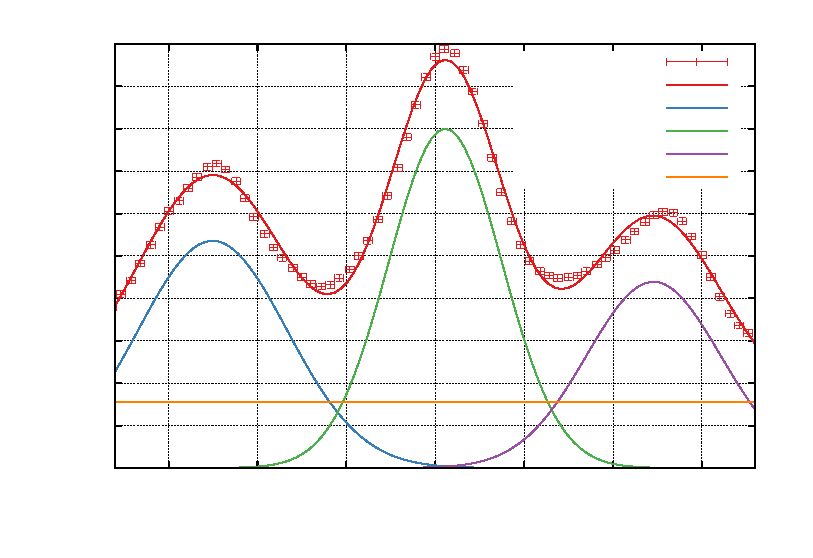
\includegraphics{./plots/zeemann_aufspaltung/b8-5}}%
    \gplfronttext
  \end{picture}%
\endgroup

	\caption{8.5A}
	\label{fig:gauss10}
\end{figure}

\begin{figure}[h]
	\centering
	% GNUPLOT: LaTeX picture with Postscript
\begingroup
  \makeatletter
  \providecommand\color[2][]{%
    \GenericError{(gnuplot) \space\space\space\@spaces}{%
      Package color not loaded in conjunction with
      terminal option `colourtext'%
    }{See the gnuplot documentation for explanation.%
    }{Either use 'blacktext' in gnuplot or load the package
      color.sty in LaTeX.}%
    \renewcommand\color[2][]{}%
  }%
  \providecommand\includegraphics[2][]{%
    \GenericError{(gnuplot) \space\space\space\@spaces}{%
      Package graphicx or graphics not loaded%
    }{See the gnuplot documentation for explanation.%
    }{The gnuplot epslatex terminal needs graphicx.sty or graphics.sty.}%
    \renewcommand\includegraphics[2][]{}%
  }%
  \providecommand\rotatebox[2]{#2}%
  \@ifundefined{ifGPcolor}{%
    \newif\ifGPcolor
    \GPcolortrue
  }{}%
  \@ifundefined{ifGPblacktext}{%
    \newif\ifGPblacktext
    \GPblacktexttrue
  }{}%
  % define a \g@addto@macro without @ in the name:
  \let\gplgaddtomacro\g@addto@macro
  % define empty templates for all commands taking text:
  \gdef\gplbacktext{}%
  \gdef\gplfronttext{}%
  \makeatother
  \ifGPblacktext
    % no textcolor at all
    \def\colorrgb#1{}%
    \def\colorgray#1{}%
  \else
    % gray or color?
    \ifGPcolor
      \def\colorrgb#1{\color[rgb]{#1}}%
      \def\colorgray#1{\color[gray]{#1}}%
      \expandafter\def\csname LTw\endcsname{\color{white}}%
      \expandafter\def\csname LTb\endcsname{\color{black}}%
      \expandafter\def\csname LTa\endcsname{\color{black}}%
      \expandafter\def\csname LT0\endcsname{\color[rgb]{1,0,0}}%
      \expandafter\def\csname LT1\endcsname{\color[rgb]{0,1,0}}%
      \expandafter\def\csname LT2\endcsname{\color[rgb]{0,0,1}}%
      \expandafter\def\csname LT3\endcsname{\color[rgb]{1,0,1}}%
      \expandafter\def\csname LT4\endcsname{\color[rgb]{0,1,1}}%
      \expandafter\def\csname LT5\endcsname{\color[rgb]{1,1,0}}%
      \expandafter\def\csname LT6\endcsname{\color[rgb]{0,0,0}}%
      \expandafter\def\csname LT7\endcsname{\color[rgb]{1,0.3,0}}%
      \expandafter\def\csname LT8\endcsname{\color[rgb]{0.5,0.5,0.5}}%
    \else
      % gray
      \def\colorrgb#1{\color{black}}%
      \def\colorgray#1{\color[gray]{#1}}%
      \expandafter\def\csname LTw\endcsname{\color{white}}%
      \expandafter\def\csname LTb\endcsname{\color{black}}%
      \expandafter\def\csname LTa\endcsname{\color{black}}%
      \expandafter\def\csname LT0\endcsname{\color{black}}%
      \expandafter\def\csname LT1\endcsname{\color{black}}%
      \expandafter\def\csname LT2\endcsname{\color{black}}%
      \expandafter\def\csname LT3\endcsname{\color{black}}%
      \expandafter\def\csname LT4\endcsname{\color{black}}%
      \expandafter\def\csname LT5\endcsname{\color{black}}%
      \expandafter\def\csname LT6\endcsname{\color{black}}%
      \expandafter\def\csname LT7\endcsname{\color{black}}%
      \expandafter\def\csname LT8\endcsname{\color{black}}%
    \fi
  \fi
  \setlength{\unitlength}{0.0500bp}%
  \begin{picture}(7488.00,5040.00)%
    \gplgaddtomacro\gplbacktext{%
      \csname LTb\endcsname%
      \put(814,704){\makebox(0,0)[r]{\strut{} 0}}%
      \csname LTb\endcsname%
      \put(814,1383){\makebox(0,0)[r]{\strut{} 10}}%
      \csname LTb\endcsname%
      \put(814,2061){\makebox(0,0)[r]{\strut{} 20}}%
      \csname LTb\endcsname%
      \put(814,2740){\makebox(0,0)[r]{\strut{} 30}}%
      \csname LTb\endcsname%
      \put(814,3418){\makebox(0,0)[r]{\strut{} 40}}%
      \csname LTb\endcsname%
      \put(814,4097){\makebox(0,0)[r]{\strut{} 50}}%
      \csname LTb\endcsname%
      \put(814,4775){\makebox(0,0)[r]{\strut{} 60}}%
      \csname LTb\endcsname%
      \put(1458,484){\makebox(0,0){\strut{} 0.85}}%
      \csname LTb\endcsname%
      \put(2312,484){\makebox(0,0){\strut{} 0.9}}%
      \csname LTb\endcsname%
      \put(3165,484){\makebox(0,0){\strut{} 0.95}}%
      \csname LTb\endcsname%
      \put(4019,484){\makebox(0,0){\strut{} 1}}%
      \csname LTb\endcsname%
      \put(4872,484){\makebox(0,0){\strut{} 1.05}}%
      \csname LTb\endcsname%
      \put(5725,484){\makebox(0,0){\strut{} 1.1}}%
      \csname LTb\endcsname%
      \put(6579,484){\makebox(0,0){\strut{} 1.15}}%
      \put(176,2739){\rotatebox{-270}{\makebox(0,0){\strut{}Intensität $I$ / \si{\percent}}}}%
      \put(4018,154){\makebox(0,0){\strut{}Winkel $\alpha$ / \si{\degree}}}%
      \put(4018,4665){\makebox(0,0){\strut{}}}%
    }%
    \gplgaddtomacro\gplfronttext{%
      \csname LTb\endcsname%
      \put(6104,4602){\makebox(0,0)[r]{\strut{}Messwerte}}%
      \csname LTb\endcsname%
      \put(6104,4382){\makebox(0,0)[r]{\strut{}$\Sigma$}}%
      \csname LTb\endcsname%
      \put(6104,4162){\makebox(0,0)[r]{\strut{}$\mathcal{G}_1$}}%
      \csname LTb\endcsname%
      \put(6104,3942){\makebox(0,0)[r]{\strut{}$\mathcal{G}_2$}}%
      \csname LTb\endcsname%
      \put(6104,3722){\makebox(0,0)[r]{\strut{}$\mathcal{G}_3$}}%
      \csname LTb\endcsname%
      \put(6104,3502){\makebox(0,0)[r]{\strut{}$d$}}%
    }%
    \gplbacktext
    \put(0,0){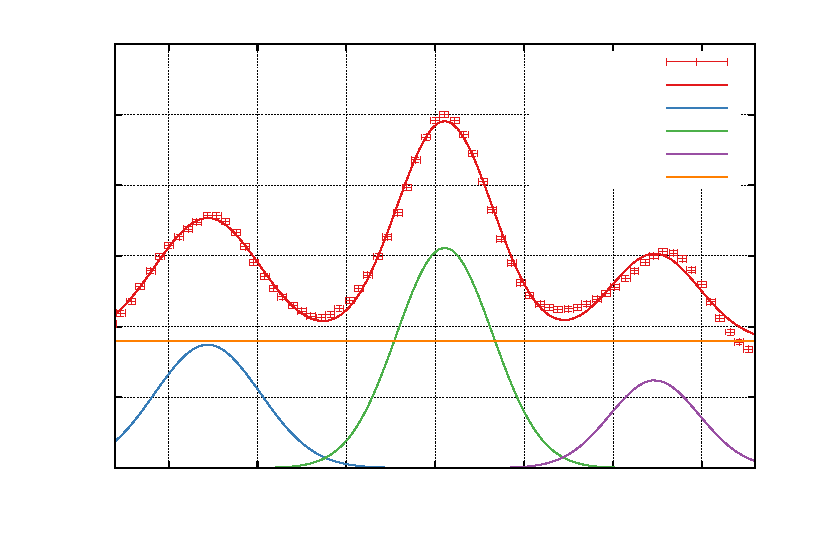
\includegraphics{./plots/zeemann_aufspaltung/b8-9}}%
    \gplfronttext
  \end{picture}%
\endgroup

	\caption{8.9A}
	\label{fig:gauss11}
\end{figure}

\FloatBarrier

=======
\begin{figure}[h]
\centering
% GNUPLOT: LaTeX picture with Postscript
\begingroup
  \makeatletter
  \providecommand\color[2][]{%
    \GenericError{(gnuplot) \space\space\space\@spaces}{%
      Package color not loaded in conjunction with
      terminal option `colourtext'%
    }{See the gnuplot documentation for explanation.%
    }{Either use 'blacktext' in gnuplot or load the package
      color.sty in LaTeX.}%
    \renewcommand\color[2][]{}%
  }%
  \providecommand\includegraphics[2][]{%
    \GenericError{(gnuplot) \space\space\space\@spaces}{%
      Package graphicx or graphics not loaded%
    }{See the gnuplot documentation for explanation.%
    }{The gnuplot epslatex terminal needs graphicx.sty or graphics.sty.}%
    \renewcommand\includegraphics[2][]{}%
  }%
  \providecommand\rotatebox[2]{#2}%
  \@ifundefined{ifGPcolor}{%
    \newif\ifGPcolor
    \GPcolortrue
  }{}%
  \@ifundefined{ifGPblacktext}{%
    \newif\ifGPblacktext
    \GPblacktexttrue
  }{}%
  % define a \g@addto@macro without @ in the name:
  \let\gplgaddtomacro\g@addto@macro
  % define empty templates for all commands taking text:
  \gdef\gplbacktext{}%
  \gdef\gplfronttext{}%
  \makeatother
  \ifGPblacktext
    % no textcolor at all
    \def\colorrgb#1{}%
    \def\colorgray#1{}%
  \else
    % gray or color?
    \ifGPcolor
      \def\colorrgb#1{\color[rgb]{#1}}%
      \def\colorgray#1{\color[gray]{#1}}%
      \expandafter\def\csname LTw\endcsname{\color{white}}%
      \expandafter\def\csname LTb\endcsname{\color{black}}%
      \expandafter\def\csname LTa\endcsname{\color{black}}%
      \expandafter\def\csname LT0\endcsname{\color[rgb]{1,0,0}}%
      \expandafter\def\csname LT1\endcsname{\color[rgb]{0,1,0}}%
      \expandafter\def\csname LT2\endcsname{\color[rgb]{0,0,1}}%
      \expandafter\def\csname LT3\endcsname{\color[rgb]{1,0,1}}%
      \expandafter\def\csname LT4\endcsname{\color[rgb]{0,1,1}}%
      \expandafter\def\csname LT5\endcsname{\color[rgb]{1,1,0}}%
      \expandafter\def\csname LT6\endcsname{\color[rgb]{0,0,0}}%
      \expandafter\def\csname LT7\endcsname{\color[rgb]{1,0.3,0}}%
      \expandafter\def\csname LT8\endcsname{\color[rgb]{0.5,0.5,0.5}}%
    \else
      % gray
      \def\colorrgb#1{\color{black}}%
      \def\colorgray#1{\color[gray]{#1}}%
      \expandafter\def\csname LTw\endcsname{\color{white}}%
      \expandafter\def\csname LTb\endcsname{\color{black}}%
      \expandafter\def\csname LTa\endcsname{\color{black}}%
      \expandafter\def\csname LT0\endcsname{\color{black}}%
      \expandafter\def\csname LT1\endcsname{\color{black}}%
      \expandafter\def\csname LT2\endcsname{\color{black}}%
      \expandafter\def\csname LT3\endcsname{\color{black}}%
      \expandafter\def\csname LT4\endcsname{\color{black}}%
      \expandafter\def\csname LT5\endcsname{\color{black}}%
      \expandafter\def\csname LT6\endcsname{\color{black}}%
      \expandafter\def\csname LT7\endcsname{\color{black}}%
      \expandafter\def\csname LT8\endcsname{\color{black}}%
    \fi
  \fi
  \setlength{\unitlength}{0.0500bp}%
  \begin{picture}(7488.00,5040.00)%
    \gplgaddtomacro\gplbacktext{%
      \csname LTb\endcsname%
      \put(814,704){\makebox(0,0)[r]{\strut{} 0}}%
      \csname LTb\endcsname%
      \put(814,1111){\makebox(0,0)[r]{\strut{} 5}}%
      \csname LTb\endcsname%
      \put(814,1518){\makebox(0,0)[r]{\strut{} 10}}%
      \csname LTb\endcsname%
      \put(814,1925){\makebox(0,0)[r]{\strut{} 15}}%
      \csname LTb\endcsname%
      \put(814,2332){\makebox(0,0)[r]{\strut{} 20}}%
      \csname LTb\endcsname%
      \put(814,2740){\makebox(0,0)[r]{\strut{} 25}}%
      \csname LTb\endcsname%
      \put(814,3147){\makebox(0,0)[r]{\strut{} 30}}%
      \csname LTb\endcsname%
      \put(814,3554){\makebox(0,0)[r]{\strut{} 35}}%
      \csname LTb\endcsname%
      \put(814,3961){\makebox(0,0)[r]{\strut{} 40}}%
      \csname LTb\endcsname%
      \put(814,4368){\makebox(0,0)[r]{\strut{} 45}}%
      \csname LTb\endcsname%
      \put(814,4775){\makebox(0,0)[r]{\strut{} 50}}%
      \csname LTb\endcsname%
      \put(1307,484){\makebox(0,0){\strut{} 0.85}}%
      \csname LTb\endcsname%
      \put(2211,484){\makebox(0,0){\strut{} 0.9}}%
      \csname LTb\endcsname%
      \put(3115,484){\makebox(0,0){\strut{} 0.95}}%
      \csname LTb\endcsname%
      \put(4019,484){\makebox(0,0){\strut{} 1}}%
      \csname LTb\endcsname%
      \put(4922,484){\makebox(0,0){\strut{} 1.05}}%
      \csname LTb\endcsname%
      \put(5826,484){\makebox(0,0){\strut{} 1.1}}%
      \csname LTb\endcsname%
      \put(6730,484){\makebox(0,0){\strut{} 1.15}}%
      \put(176,2739){\rotatebox{-270}{\makebox(0,0){\strut{}Intensität $I$ / \si{\percent}}}}%
      \put(4018,154){\makebox(0,0){\strut{}Winkel $\alpha$ / \si{\degree}}}%
      \put(4018,4665){\makebox(0,0){\strut{}}}%
    }%
    \gplgaddtomacro\gplfronttext{%
      \csname LTb\endcsname%
      \put(6104,4602){\makebox(0,0)[r]{\strut{}Messwerte}}%
      \csname LTb\endcsname%
      \put(6104,4382){\makebox(0,0)[r]{\strut{}$\Sigma$}}%
      \csname LTb\endcsname%
      \put(6104,4162){\makebox(0,0)[r]{\strut{}$\mathcal{G}_1$}}%
      \csname LTb\endcsname%
      \put(6104,3942){\makebox(0,0)[r]{\strut{}$\mathcal{G}_2$}}%
      \csname LTb\endcsname%
      \put(6104,3722){\makebox(0,0)[r]{\strut{}$\mathcal{G}_3$}}%
      \csname LTb\endcsname%
      \put(6104,3502){\makebox(0,0)[r]{\strut{}$d$}}%
    }%
    \gplbacktext
    \put(0,0){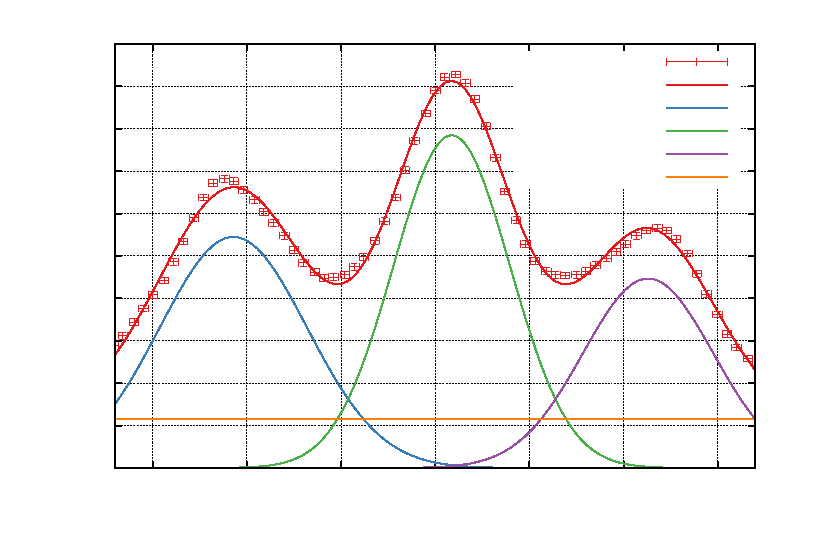
\includegraphics{./plots/zeemann_aufspaltung/b6-5}}%
    \gplfronttext
  \end{picture}%
\endgroup

\caption{6.5A}
\label{fig:gauss6}
\end{figure}

\begin{figure}[h]
\centering
% GNUPLOT: LaTeX picture with Postscript
\begingroup
  \makeatletter
  \providecommand\color[2][]{%
    \GenericError{(gnuplot) \space\space\space\@spaces}{%
      Package color not loaded in conjunction with
      terminal option `colourtext'%
    }{See the gnuplot documentation for explanation.%
    }{Either use 'blacktext' in gnuplot or load the package
      color.sty in LaTeX.}%
    \renewcommand\color[2][]{}%
  }%
  \providecommand\includegraphics[2][]{%
    \GenericError{(gnuplot) \space\space\space\@spaces}{%
      Package graphicx or graphics not loaded%
    }{See the gnuplot documentation for explanation.%
    }{The gnuplot epslatex terminal needs graphicx.sty or graphics.sty.}%
    \renewcommand\includegraphics[2][]{}%
  }%
  \providecommand\rotatebox[2]{#2}%
  \@ifundefined{ifGPcolor}{%
    \newif\ifGPcolor
    \GPcolortrue
  }{}%
  \@ifundefined{ifGPblacktext}{%
    \newif\ifGPblacktext
    \GPblacktexttrue
  }{}%
  % define a \g@addto@macro without @ in the name:
  \let\gplgaddtomacro\g@addto@macro
  % define empty templates for all commands taking text:
  \gdef\gplbacktext{}%
  \gdef\gplfronttext{}%
  \makeatother
  \ifGPblacktext
    % no textcolor at all
    \def\colorrgb#1{}%
    \def\colorgray#1{}%
  \else
    % gray or color?
    \ifGPcolor
      \def\colorrgb#1{\color[rgb]{#1}}%
      \def\colorgray#1{\color[gray]{#1}}%
      \expandafter\def\csname LTw\endcsname{\color{white}}%
      \expandafter\def\csname LTb\endcsname{\color{black}}%
      \expandafter\def\csname LTa\endcsname{\color{black}}%
      \expandafter\def\csname LT0\endcsname{\color[rgb]{1,0,0}}%
      \expandafter\def\csname LT1\endcsname{\color[rgb]{0,1,0}}%
      \expandafter\def\csname LT2\endcsname{\color[rgb]{0,0,1}}%
      \expandafter\def\csname LT3\endcsname{\color[rgb]{1,0,1}}%
      \expandafter\def\csname LT4\endcsname{\color[rgb]{0,1,1}}%
      \expandafter\def\csname LT5\endcsname{\color[rgb]{1,1,0}}%
      \expandafter\def\csname LT6\endcsname{\color[rgb]{0,0,0}}%
      \expandafter\def\csname LT7\endcsname{\color[rgb]{1,0.3,0}}%
      \expandafter\def\csname LT8\endcsname{\color[rgb]{0.5,0.5,0.5}}%
    \else
      % gray
      \def\colorrgb#1{\color{black}}%
      \def\colorgray#1{\color[gray]{#1}}%
      \expandafter\def\csname LTw\endcsname{\color{white}}%
      \expandafter\def\csname LTb\endcsname{\color{black}}%
      \expandafter\def\csname LTa\endcsname{\color{black}}%
      \expandafter\def\csname LT0\endcsname{\color{black}}%
      \expandafter\def\csname LT1\endcsname{\color{black}}%
      \expandafter\def\csname LT2\endcsname{\color{black}}%
      \expandafter\def\csname LT3\endcsname{\color{black}}%
      \expandafter\def\csname LT4\endcsname{\color{black}}%
      \expandafter\def\csname LT5\endcsname{\color{black}}%
      \expandafter\def\csname LT6\endcsname{\color{black}}%
      \expandafter\def\csname LT7\endcsname{\color{black}}%
      \expandafter\def\csname LT8\endcsname{\color{black}}%
    \fi
  \fi
  \setlength{\unitlength}{0.0500bp}%
  \begin{picture}(7486.00,5040.00)%
    \gplgaddtomacro\gplbacktext{%
      \csname LTb\endcsname%
      \put(814,704){\makebox(0,0)[r]{\strut{} 0}}%
      \csname LTb\endcsname%
      \put(814,1111){\makebox(0,0)[r]{\strut{} 5}}%
      \csname LTb\endcsname%
      \put(814,1518){\makebox(0,0)[r]{\strut{} 10}}%
      \csname LTb\endcsname%
      \put(814,1925){\makebox(0,0)[r]{\strut{} 15}}%
      \csname LTb\endcsname%
      \put(814,2332){\makebox(0,0)[r]{\strut{} 20}}%
      \csname LTb\endcsname%
      \put(814,2740){\makebox(0,0)[r]{\strut{} 25}}%
      \csname LTb\endcsname%
      \put(814,3147){\makebox(0,0)[r]{\strut{} 30}}%
      \csname LTb\endcsname%
      \put(814,3554){\makebox(0,0)[r]{\strut{} 35}}%
      \csname LTb\endcsname%
      \put(814,3961){\makebox(0,0)[r]{\strut{} 40}}%
      \csname LTb\endcsname%
      \put(814,4368){\makebox(0,0)[r]{\strut{} 45}}%
      \csname LTb\endcsname%
      \put(814,4775){\makebox(0,0)[r]{\strut{} 50}}%
      \csname LTb\endcsname%
      \put(946,484){\makebox(0,0){\strut{} 0.8}}%
      \csname LTb\endcsname%
      \put(1714,484){\makebox(0,0){\strut{} 0.85}}%
      \csname LTb\endcsname%
      \put(2482,484){\makebox(0,0){\strut{} 0.9}}%
      \csname LTb\endcsname%
      \put(3250,484){\makebox(0,0){\strut{} 0.95}}%
      \csname LTb\endcsname%
      \put(4018,484){\makebox(0,0){\strut{} 1}}%
      \csname LTb\endcsname%
      \put(4785,484){\makebox(0,0){\strut{} 1.05}}%
      \csname LTb\endcsname%
      \put(5553,484){\makebox(0,0){\strut{} 1.1}}%
      \csname LTb\endcsname%
      \put(6321,484){\makebox(0,0){\strut{} 1.15}}%
      \csname LTb\endcsname%
      \put(7089,484){\makebox(0,0){\strut{} 1.2}}%
      \put(176,2739){\rotatebox{-270}{\makebox(0,0){\strut{}Intensität $I$ / \si{\percent}}}}%
      \put(4017,154){\makebox(0,0){\strut{}Winkel $\alpha$ / \si{\degree}}}%
      \put(4017,4665){\makebox(0,0){\strut{}}}%
    }%
    \gplgaddtomacro\gplfronttext{%
      \csname LTb\endcsname%
      \put(6102,4602){\makebox(0,0)[r]{\strut{}Messwerte}}%
      \csname LTb\endcsname%
      \put(6102,4382){\makebox(0,0)[r]{\strut{}$\Sigma$}}%
      \csname LTb\endcsname%
      \put(6102,4162){\makebox(0,0)[r]{\strut{}$\mathcal{G}_1$}}%
      \csname LTb\endcsname%
      \put(6102,3942){\makebox(0,0)[r]{\strut{}$\mathcal{G}_2$}}%
      \csname LTb\endcsname%
      \put(6102,3722){\makebox(0,0)[r]{\strut{}$\mathcal{G}_3$}}%
      \csname LTb\endcsname%
      \put(6102,3502){\makebox(0,0)[r]{\strut{}Untergrund}}%
    }%
    \gplbacktext
    \put(0,0){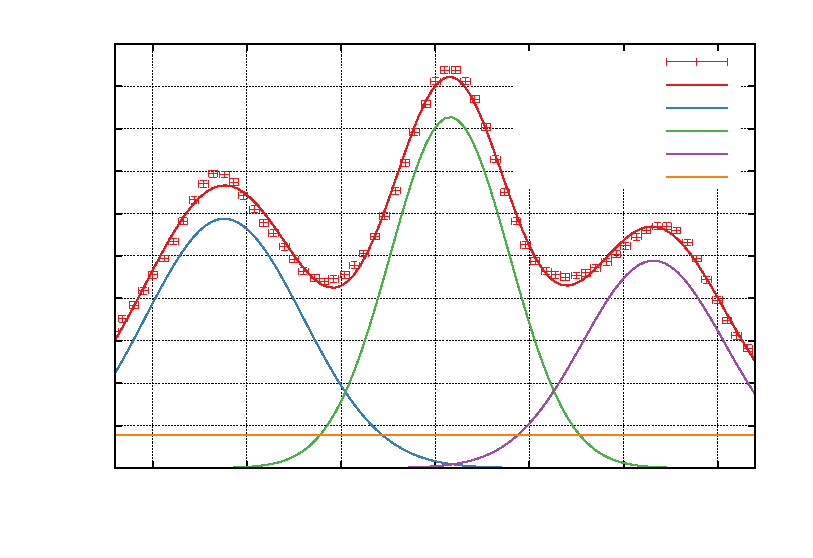
\includegraphics{./plots/zeemann_aufspaltung/b7}}%
    \gplfronttext
  \end{picture}%
\endgroup

\caption{7 A}
\label{fig:gauss7}
\end{figure}

\begin{figure}[h]
\centering
% GNUPLOT: LaTeX picture with Postscript
\begingroup
  \makeatletter
  \providecommand\color[2][]{%
    \GenericError{(gnuplot) \space\space\space\@spaces}{%
      Package color not loaded in conjunction with
      terminal option `colourtext'%
    }{See the gnuplot documentation for explanation.%
    }{Either use 'blacktext' in gnuplot or load the package
      color.sty in LaTeX.}%
    \renewcommand\color[2][]{}%
  }%
  \providecommand\includegraphics[2][]{%
    \GenericError{(gnuplot) \space\space\space\@spaces}{%
      Package graphicx or graphics not loaded%
    }{See the gnuplot documentation for explanation.%
    }{The gnuplot epslatex terminal needs graphicx.sty or graphics.sty.}%
    \renewcommand\includegraphics[2][]{}%
  }%
  \providecommand\rotatebox[2]{#2}%
  \@ifundefined{ifGPcolor}{%
    \newif\ifGPcolor
    \GPcolortrue
  }{}%
  \@ifundefined{ifGPblacktext}{%
    \newif\ifGPblacktext
    \GPblacktexttrue
  }{}%
  % define a \g@addto@macro without @ in the name:
  \let\gplgaddtomacro\g@addto@macro
  % define empty templates for all commands taking text:
  \gdef\gplbacktext{}%
  \gdef\gplfronttext{}%
  \makeatother
  \ifGPblacktext
    % no textcolor at all
    \def\colorrgb#1{}%
    \def\colorgray#1{}%
  \else
    % gray or color?
    \ifGPcolor
      \def\colorrgb#1{\color[rgb]{#1}}%
      \def\colorgray#1{\color[gray]{#1}}%
      \expandafter\def\csname LTw\endcsname{\color{white}}%
      \expandafter\def\csname LTb\endcsname{\color{black}}%
      \expandafter\def\csname LTa\endcsname{\color{black}}%
      \expandafter\def\csname LT0\endcsname{\color[rgb]{1,0,0}}%
      \expandafter\def\csname LT1\endcsname{\color[rgb]{0,1,0}}%
      \expandafter\def\csname LT2\endcsname{\color[rgb]{0,0,1}}%
      \expandafter\def\csname LT3\endcsname{\color[rgb]{1,0,1}}%
      \expandafter\def\csname LT4\endcsname{\color[rgb]{0,1,1}}%
      \expandafter\def\csname LT5\endcsname{\color[rgb]{1,1,0}}%
      \expandafter\def\csname LT6\endcsname{\color[rgb]{0,0,0}}%
      \expandafter\def\csname LT7\endcsname{\color[rgb]{1,0.3,0}}%
      \expandafter\def\csname LT8\endcsname{\color[rgb]{0.5,0.5,0.5}}%
    \else
      % gray
      \def\colorrgb#1{\color{black}}%
      \def\colorgray#1{\color[gray]{#1}}%
      \expandafter\def\csname LTw\endcsname{\color{white}}%
      \expandafter\def\csname LTb\endcsname{\color{black}}%
      \expandafter\def\csname LTa\endcsname{\color{black}}%
      \expandafter\def\csname LT0\endcsname{\color{black}}%
      \expandafter\def\csname LT1\endcsname{\color{black}}%
      \expandafter\def\csname LT2\endcsname{\color{black}}%
      \expandafter\def\csname LT3\endcsname{\color{black}}%
      \expandafter\def\csname LT4\endcsname{\color{black}}%
      \expandafter\def\csname LT5\endcsname{\color{black}}%
      \expandafter\def\csname LT6\endcsname{\color{black}}%
      \expandafter\def\csname LT7\endcsname{\color{black}}%
      \expandafter\def\csname LT8\endcsname{\color{black}}%
    \fi
  \fi
  \setlength{\unitlength}{0.0500bp}%
  \begin{picture}(7488.00,5040.00)%
    \gplgaddtomacro\gplbacktext{%
      \csname LTb\endcsname%
      \put(814,704){\makebox(0,0)[r]{\strut{} 0}}%
      \csname LTb\endcsname%
      \put(814,1111){\makebox(0,0)[r]{\strut{} 5}}%
      \csname LTb\endcsname%
      \put(814,1518){\makebox(0,0)[r]{\strut{} 10}}%
      \csname LTb\endcsname%
      \put(814,1925){\makebox(0,0)[r]{\strut{} 15}}%
      \csname LTb\endcsname%
      \put(814,2332){\makebox(0,0)[r]{\strut{} 20}}%
      \csname LTb\endcsname%
      \put(814,2740){\makebox(0,0)[r]{\strut{} 25}}%
      \csname LTb\endcsname%
      \put(814,3147){\makebox(0,0)[r]{\strut{} 30}}%
      \csname LTb\endcsname%
      \put(814,3554){\makebox(0,0)[r]{\strut{} 35}}%
      \csname LTb\endcsname%
      \put(814,3961){\makebox(0,0)[r]{\strut{} 40}}%
      \csname LTb\endcsname%
      \put(814,4368){\makebox(0,0)[r]{\strut{} 45}}%
      \csname LTb\endcsname%
      \put(814,4775){\makebox(0,0)[r]{\strut{} 50}}%
      \csname LTb\endcsname%
      \put(1307,484){\makebox(0,0){\strut{} 0.85}}%
      \csname LTb\endcsname%
      \put(2211,484){\makebox(0,0){\strut{} 0.9}}%
      \csname LTb\endcsname%
      \put(3115,484){\makebox(0,0){\strut{} 0.95}}%
      \csname LTb\endcsname%
      \put(4019,484){\makebox(0,0){\strut{} 1}}%
      \csname LTb\endcsname%
      \put(4922,484){\makebox(0,0){\strut{} 1.05}}%
      \csname LTb\endcsname%
      \put(5826,484){\makebox(0,0){\strut{} 1.1}}%
      \csname LTb\endcsname%
      \put(6730,484){\makebox(0,0){\strut{} 1.15}}%
      \put(176,2739){\rotatebox{-270}{\makebox(0,0){\strut{}Intensität $I$ / \si{\percent}}}}%
      \put(4018,154){\makebox(0,0){\strut{}Winkel $\alpha$ / \si{\degree}}}%
      \put(4018,4665){\makebox(0,0){\strut{}}}%
    }%
    \gplgaddtomacro\gplfronttext{%
      \csname LTb\endcsname%
      \put(6104,4602){\makebox(0,0)[r]{\strut{}Messwerte}}%
      \csname LTb\endcsname%
      \put(6104,4382){\makebox(0,0)[r]{\strut{}$\Sigma$}}%
      \csname LTb\endcsname%
      \put(6104,4162){\makebox(0,0)[r]{\strut{}$\mathcal{G}_1$}}%
      \csname LTb\endcsname%
      \put(6104,3942){\makebox(0,0)[r]{\strut{}$\mathcal{G}_2$}}%
      \csname LTb\endcsname%
      \put(6104,3722){\makebox(0,0)[r]{\strut{}$\mathcal{G}_3$}}%
      \csname LTb\endcsname%
      \put(6104,3502){\makebox(0,0)[r]{\strut{}$d$}}%
    }%
    \gplbacktext
    \put(0,0){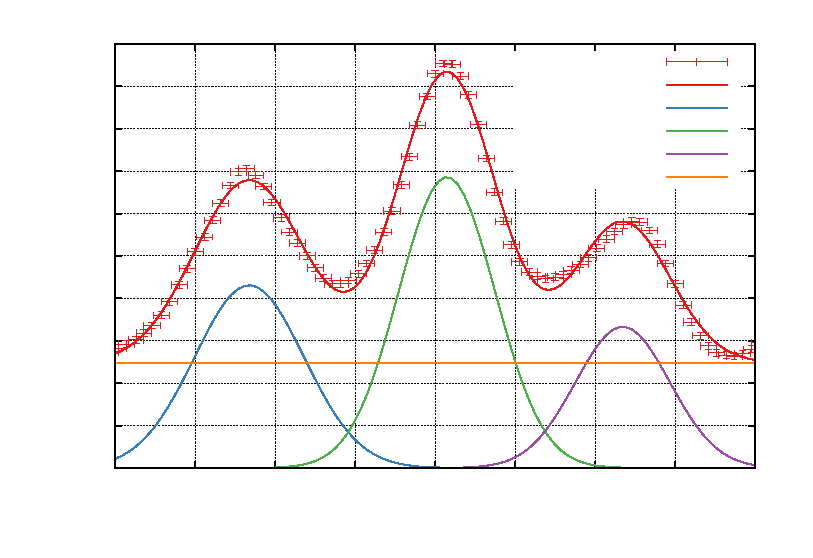
\includegraphics{./plots/zeemann_aufspaltung/b7-5}}%
    \gplfronttext
  \end{picture}%
\endgroup

\caption{7.5A}
\label{fig:gauss8}
\end{figure}

\begin{figure}[h]
\centering
% GNUPLOT: LaTeX picture with Postscript
\begingroup
  \makeatletter
  \providecommand\color[2][]{%
    \GenericError{(gnuplot) \space\space\space\@spaces}{%
      Package color not loaded in conjunction with
      terminal option `colourtext'%
    }{See the gnuplot documentation for explanation.%
    }{Either use 'blacktext' in gnuplot or load the package
      color.sty in LaTeX.}%
    \renewcommand\color[2][]{}%
  }%
  \providecommand\includegraphics[2][]{%
    \GenericError{(gnuplot) \space\space\space\@spaces}{%
      Package graphicx or graphics not loaded%
    }{See the gnuplot documentation for explanation.%
    }{The gnuplot epslatex terminal needs graphicx.sty or graphics.sty.}%
    \renewcommand\includegraphics[2][]{}%
  }%
  \providecommand\rotatebox[2]{#2}%
  \@ifundefined{ifGPcolor}{%
    \newif\ifGPcolor
    \GPcolortrue
  }{}%
  \@ifundefined{ifGPblacktext}{%
    \newif\ifGPblacktext
    \GPblacktexttrue
  }{}%
  % define a \g@addto@macro without @ in the name:
  \let\gplgaddtomacro\g@addto@macro
  % define empty templates for all commands taking text:
  \gdef\gplbacktext{}%
  \gdef\gplfronttext{}%
  \makeatother
  \ifGPblacktext
    % no textcolor at all
    \def\colorrgb#1{}%
    \def\colorgray#1{}%
  \else
    % gray or color?
    \ifGPcolor
      \def\colorrgb#1{\color[rgb]{#1}}%
      \def\colorgray#1{\color[gray]{#1}}%
      \expandafter\def\csname LTw\endcsname{\color{white}}%
      \expandafter\def\csname LTb\endcsname{\color{black}}%
      \expandafter\def\csname LTa\endcsname{\color{black}}%
      \expandafter\def\csname LT0\endcsname{\color[rgb]{1,0,0}}%
      \expandafter\def\csname LT1\endcsname{\color[rgb]{0,1,0}}%
      \expandafter\def\csname LT2\endcsname{\color[rgb]{0,0,1}}%
      \expandafter\def\csname LT3\endcsname{\color[rgb]{1,0,1}}%
      \expandafter\def\csname LT4\endcsname{\color[rgb]{0,1,1}}%
      \expandafter\def\csname LT5\endcsname{\color[rgb]{1,1,0}}%
      \expandafter\def\csname LT6\endcsname{\color[rgb]{0,0,0}}%
      \expandafter\def\csname LT7\endcsname{\color[rgb]{1,0.3,0}}%
      \expandafter\def\csname LT8\endcsname{\color[rgb]{0.5,0.5,0.5}}%
    \else
      % gray
      \def\colorrgb#1{\color{black}}%
      \def\colorgray#1{\color[gray]{#1}}%
      \expandafter\def\csname LTw\endcsname{\color{white}}%
      \expandafter\def\csname LTb\endcsname{\color{black}}%
      \expandafter\def\csname LTa\endcsname{\color{black}}%
      \expandafter\def\csname LT0\endcsname{\color{black}}%
      \expandafter\def\csname LT1\endcsname{\color{black}}%
      \expandafter\def\csname LT2\endcsname{\color{black}}%
      \expandafter\def\csname LT3\endcsname{\color{black}}%
      \expandafter\def\csname LT4\endcsname{\color{black}}%
      \expandafter\def\csname LT5\endcsname{\color{black}}%
      \expandafter\def\csname LT6\endcsname{\color{black}}%
      \expandafter\def\csname LT7\endcsname{\color{black}}%
      \expandafter\def\csname LT8\endcsname{\color{black}}%
    \fi
  \fi
  \setlength{\unitlength}{0.0500bp}%
  \begin{picture}(7486.00,5040.00)%
    \gplgaddtomacro\gplbacktext{%
      \csname LTb\endcsname%
      \put(814,704){\makebox(0,0)[r]{\strut{} 0}}%
      \csname LTb\endcsname%
      \put(814,1111){\makebox(0,0)[r]{\strut{} 5}}%
      \csname LTb\endcsname%
      \put(814,1518){\makebox(0,0)[r]{\strut{} 10}}%
      \csname LTb\endcsname%
      \put(814,1925){\makebox(0,0)[r]{\strut{} 15}}%
      \csname LTb\endcsname%
      \put(814,2332){\makebox(0,0)[r]{\strut{} 20}}%
      \csname LTb\endcsname%
      \put(814,2740){\makebox(0,0)[r]{\strut{} 25}}%
      \csname LTb\endcsname%
      \put(814,3147){\makebox(0,0)[r]{\strut{} 30}}%
      \csname LTb\endcsname%
      \put(814,3554){\makebox(0,0)[r]{\strut{} 35}}%
      \csname LTb\endcsname%
      \put(814,3961){\makebox(0,0)[r]{\strut{} 40}}%
      \csname LTb\endcsname%
      \put(814,4368){\makebox(0,0)[r]{\strut{} 45}}%
      \csname LTb\endcsname%
      \put(814,4775){\makebox(0,0)[r]{\strut{} 50}}%
      \csname LTb\endcsname%
      \put(946,484){\makebox(0,0){\strut{} 0.8}}%
      \csname LTb\endcsname%
      \put(1714,484){\makebox(0,0){\strut{} 0.85}}%
      \csname LTb\endcsname%
      \put(2482,484){\makebox(0,0){\strut{} 0.9}}%
      \csname LTb\endcsname%
      \put(3250,484){\makebox(0,0){\strut{} 0.95}}%
      \csname LTb\endcsname%
      \put(4018,484){\makebox(0,0){\strut{} 1}}%
      \csname LTb\endcsname%
      \put(4785,484){\makebox(0,0){\strut{} 1.05}}%
      \csname LTb\endcsname%
      \put(5553,484){\makebox(0,0){\strut{} 1.1}}%
      \csname LTb\endcsname%
      \put(6321,484){\makebox(0,0){\strut{} 1.15}}%
      \csname LTb\endcsname%
      \put(7089,484){\makebox(0,0){\strut{} 1.2}}%
      \put(176,2739){\rotatebox{-270}{\makebox(0,0){\strut{}Intensität $I$ / \si{\percent}}}}%
      \put(4017,154){\makebox(0,0){\strut{}Winkel $\alpha$ / \si{\degree}}}%
      \put(4017,4665){\makebox(0,0){\strut{}}}%
    }%
    \gplgaddtomacro\gplfronttext{%
      \csname LTb\endcsname%
      \put(6102,4602){\makebox(0,0)[r]{\strut{}Messwerte}}%
      \csname LTb\endcsname%
      \put(6102,4382){\makebox(0,0)[r]{\strut{}$\Sigma$}}%
      \csname LTb\endcsname%
      \put(6102,4162){\makebox(0,0)[r]{\strut{}$\mathcal{G}_1$}}%
      \csname LTb\endcsname%
      \put(6102,3942){\makebox(0,0)[r]{\strut{}$\mathcal{G}_2$}}%
      \csname LTb\endcsname%
      \put(6102,3722){\makebox(0,0)[r]{\strut{}$\mathcal{G}_3$}}%
      \csname LTb\endcsname%
      \put(6102,3502){\makebox(0,0)[r]{\strut{}Untergrund}}%
    }%
    \gplbacktext
    \put(0,0){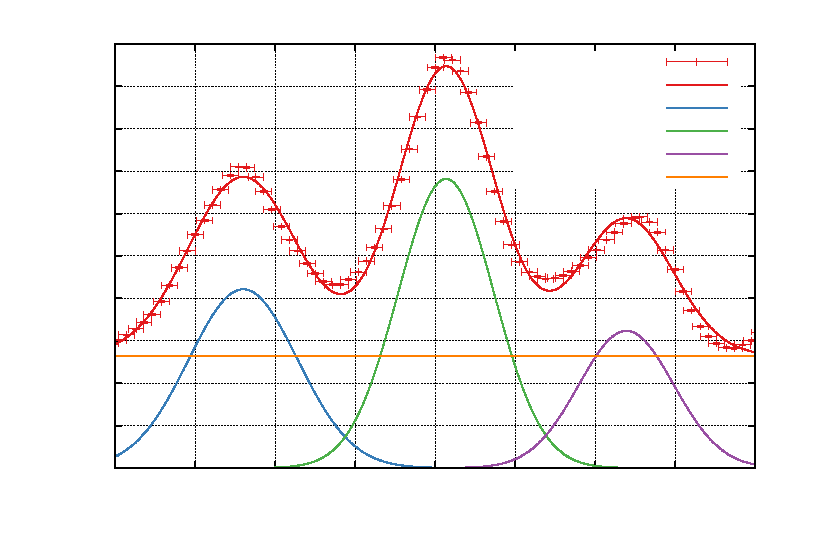
\includegraphics{./plots/zeemann_aufspaltung/b8}}%
    \gplfronttext
  \end{picture}%
\endgroup

\caption{8A}
\label{fig:gauss9}
\end{figure}

\begin{figure}[h]
\centering
% GNUPLOT: LaTeX picture with Postscript
\begingroup
  \makeatletter
  \providecommand\color[2][]{%
    \GenericError{(gnuplot) \space\space\space\@spaces}{%
      Package color not loaded in conjunction with
      terminal option `colourtext'%
    }{See the gnuplot documentation for explanation.%
    }{Either use 'blacktext' in gnuplot or load the package
      color.sty in LaTeX.}%
    \renewcommand\color[2][]{}%
  }%
  \providecommand\includegraphics[2][]{%
    \GenericError{(gnuplot) \space\space\space\@spaces}{%
      Package graphicx or graphics not loaded%
    }{See the gnuplot documentation for explanation.%
    }{The gnuplot epslatex terminal needs graphicx.sty or graphics.sty.}%
    \renewcommand\includegraphics[2][]{}%
  }%
  \providecommand\rotatebox[2]{#2}%
  \@ifundefined{ifGPcolor}{%
    \newif\ifGPcolor
    \GPcolortrue
  }{}%
  \@ifundefined{ifGPblacktext}{%
    \newif\ifGPblacktext
    \GPblacktexttrue
  }{}%
  % define a \g@addto@macro without @ in the name:
  \let\gplgaddtomacro\g@addto@macro
  % define empty templates for all commands taking text:
  \gdef\gplbacktext{}%
  \gdef\gplfronttext{}%
  \makeatother
  \ifGPblacktext
    % no textcolor at all
    \def\colorrgb#1{}%
    \def\colorgray#1{}%
  \else
    % gray or color?
    \ifGPcolor
      \def\colorrgb#1{\color[rgb]{#1}}%
      \def\colorgray#1{\color[gray]{#1}}%
      \expandafter\def\csname LTw\endcsname{\color{white}}%
      \expandafter\def\csname LTb\endcsname{\color{black}}%
      \expandafter\def\csname LTa\endcsname{\color{black}}%
      \expandafter\def\csname LT0\endcsname{\color[rgb]{1,0,0}}%
      \expandafter\def\csname LT1\endcsname{\color[rgb]{0,1,0}}%
      \expandafter\def\csname LT2\endcsname{\color[rgb]{0,0,1}}%
      \expandafter\def\csname LT3\endcsname{\color[rgb]{1,0,1}}%
      \expandafter\def\csname LT4\endcsname{\color[rgb]{0,1,1}}%
      \expandafter\def\csname LT5\endcsname{\color[rgb]{1,1,0}}%
      \expandafter\def\csname LT6\endcsname{\color[rgb]{0,0,0}}%
      \expandafter\def\csname LT7\endcsname{\color[rgb]{1,0.3,0}}%
      \expandafter\def\csname LT8\endcsname{\color[rgb]{0.5,0.5,0.5}}%
    \else
      % gray
      \def\colorrgb#1{\color{black}}%
      \def\colorgray#1{\color[gray]{#1}}%
      \expandafter\def\csname LTw\endcsname{\color{white}}%
      \expandafter\def\csname LTb\endcsname{\color{black}}%
      \expandafter\def\csname LTa\endcsname{\color{black}}%
      \expandafter\def\csname LT0\endcsname{\color{black}}%
      \expandafter\def\csname LT1\endcsname{\color{black}}%
      \expandafter\def\csname LT2\endcsname{\color{black}}%
      \expandafter\def\csname LT3\endcsname{\color{black}}%
      \expandafter\def\csname LT4\endcsname{\color{black}}%
      \expandafter\def\csname LT5\endcsname{\color{black}}%
      \expandafter\def\csname LT6\endcsname{\color{black}}%
      \expandafter\def\csname LT7\endcsname{\color{black}}%
      \expandafter\def\csname LT8\endcsname{\color{black}}%
    \fi
  \fi
  \setlength{\unitlength}{0.0500bp}%
  \begin{picture}(7488.00,5040.00)%
    \gplgaddtomacro\gplbacktext{%
      \csname LTb\endcsname%
      \put(814,704){\makebox(0,0)[r]{\strut{} 0}}%
      \csname LTb\endcsname%
      \put(814,1111){\makebox(0,0)[r]{\strut{} 5}}%
      \csname LTb\endcsname%
      \put(814,1518){\makebox(0,0)[r]{\strut{} 10}}%
      \csname LTb\endcsname%
      \put(814,1925){\makebox(0,0)[r]{\strut{} 15}}%
      \csname LTb\endcsname%
      \put(814,2332){\makebox(0,0)[r]{\strut{} 20}}%
      \csname LTb\endcsname%
      \put(814,2740){\makebox(0,0)[r]{\strut{} 25}}%
      \csname LTb\endcsname%
      \put(814,3147){\makebox(0,0)[r]{\strut{} 30}}%
      \csname LTb\endcsname%
      \put(814,3554){\makebox(0,0)[r]{\strut{} 35}}%
      \csname LTb\endcsname%
      \put(814,3961){\makebox(0,0)[r]{\strut{} 40}}%
      \csname LTb\endcsname%
      \put(814,4368){\makebox(0,0)[r]{\strut{} 45}}%
      \csname LTb\endcsname%
      \put(814,4775){\makebox(0,0)[r]{\strut{} 50}}%
      \csname LTb\endcsname%
      \put(1458,484){\makebox(0,0){\strut{} 0.85}}%
      \csname LTb\endcsname%
      \put(2312,484){\makebox(0,0){\strut{} 0.9}}%
      \csname LTb\endcsname%
      \put(3165,484){\makebox(0,0){\strut{} 0.95}}%
      \csname LTb\endcsname%
      \put(4019,484){\makebox(0,0){\strut{} 1}}%
      \csname LTb\endcsname%
      \put(4872,484){\makebox(0,0){\strut{} 1.05}}%
      \csname LTb\endcsname%
      \put(5725,484){\makebox(0,0){\strut{} 1.1}}%
      \csname LTb\endcsname%
      \put(6579,484){\makebox(0,0){\strut{} 1.15}}%
      \put(176,2739){\rotatebox{-270}{\makebox(0,0){\strut{}Intensität $I$ / \si{\percent}}}}%
      \put(4018,154){\makebox(0,0){\strut{}Winkel $\alpha$ / \si{\degree}}}%
      \put(4018,4665){\makebox(0,0){\strut{}}}%
    }%
    \gplgaddtomacro\gplfronttext{%
      \csname LTb\endcsname%
      \put(6104,4602){\makebox(0,0)[r]{\strut{}Messwerte}}%
      \csname LTb\endcsname%
      \put(6104,4382){\makebox(0,0)[r]{\strut{}$\Sigma$}}%
      \csname LTb\endcsname%
      \put(6104,4162){\makebox(0,0)[r]{\strut{}$\mathcal{G}_1$}}%
      \csname LTb\endcsname%
      \put(6104,3942){\makebox(0,0)[r]{\strut{}$\mathcal{G}_2$}}%
      \csname LTb\endcsname%
      \put(6104,3722){\makebox(0,0)[r]{\strut{}$\mathcal{G}_3$}}%
      \csname LTb\endcsname%
      \put(6104,3502){\makebox(0,0)[r]{\strut{}Untergrund}}%
    }%
    \gplbacktext
    \put(0,0){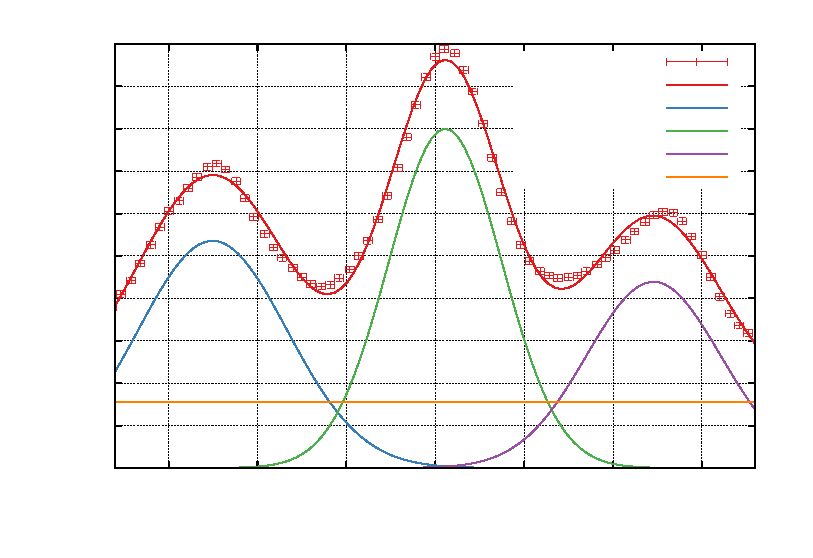
\includegraphics{./plots/zeemann_aufspaltung/b8-5}}%
    \gplfronttext
  \end{picture}%
\endgroup

\caption{8.5A}
\label{fig:gauss10}
\end{figure}

\begin{figure}[h]
\centering
% GNUPLOT: LaTeX picture with Postscript
\begingroup
  \makeatletter
  \providecommand\color[2][]{%
    \GenericError{(gnuplot) \space\space\space\@spaces}{%
      Package color not loaded in conjunction with
      terminal option `colourtext'%
    }{See the gnuplot documentation for explanation.%
    }{Either use 'blacktext' in gnuplot or load the package
      color.sty in LaTeX.}%
    \renewcommand\color[2][]{}%
  }%
  \providecommand\includegraphics[2][]{%
    \GenericError{(gnuplot) \space\space\space\@spaces}{%
      Package graphicx or graphics not loaded%
    }{See the gnuplot documentation for explanation.%
    }{The gnuplot epslatex terminal needs graphicx.sty or graphics.sty.}%
    \renewcommand\includegraphics[2][]{}%
  }%
  \providecommand\rotatebox[2]{#2}%
  \@ifundefined{ifGPcolor}{%
    \newif\ifGPcolor
    \GPcolortrue
  }{}%
  \@ifundefined{ifGPblacktext}{%
    \newif\ifGPblacktext
    \GPblacktexttrue
  }{}%
  % define a \g@addto@macro without @ in the name:
  \let\gplgaddtomacro\g@addto@macro
  % define empty templates for all commands taking text:
  \gdef\gplbacktext{}%
  \gdef\gplfronttext{}%
  \makeatother
  \ifGPblacktext
    % no textcolor at all
    \def\colorrgb#1{}%
    \def\colorgray#1{}%
  \else
    % gray or color?
    \ifGPcolor
      \def\colorrgb#1{\color[rgb]{#1}}%
      \def\colorgray#1{\color[gray]{#1}}%
      \expandafter\def\csname LTw\endcsname{\color{white}}%
      \expandafter\def\csname LTb\endcsname{\color{black}}%
      \expandafter\def\csname LTa\endcsname{\color{black}}%
      \expandafter\def\csname LT0\endcsname{\color[rgb]{1,0,0}}%
      \expandafter\def\csname LT1\endcsname{\color[rgb]{0,1,0}}%
      \expandafter\def\csname LT2\endcsname{\color[rgb]{0,0,1}}%
      \expandafter\def\csname LT3\endcsname{\color[rgb]{1,0,1}}%
      \expandafter\def\csname LT4\endcsname{\color[rgb]{0,1,1}}%
      \expandafter\def\csname LT5\endcsname{\color[rgb]{1,1,0}}%
      \expandafter\def\csname LT6\endcsname{\color[rgb]{0,0,0}}%
      \expandafter\def\csname LT7\endcsname{\color[rgb]{1,0.3,0}}%
      \expandafter\def\csname LT8\endcsname{\color[rgb]{0.5,0.5,0.5}}%
    \else
      % gray
      \def\colorrgb#1{\color{black}}%
      \def\colorgray#1{\color[gray]{#1}}%
      \expandafter\def\csname LTw\endcsname{\color{white}}%
      \expandafter\def\csname LTb\endcsname{\color{black}}%
      \expandafter\def\csname LTa\endcsname{\color{black}}%
      \expandafter\def\csname LT0\endcsname{\color{black}}%
      \expandafter\def\csname LT1\endcsname{\color{black}}%
      \expandafter\def\csname LT2\endcsname{\color{black}}%
      \expandafter\def\csname LT3\endcsname{\color{black}}%
      \expandafter\def\csname LT4\endcsname{\color{black}}%
      \expandafter\def\csname LT5\endcsname{\color{black}}%
      \expandafter\def\csname LT6\endcsname{\color{black}}%
      \expandafter\def\csname LT7\endcsname{\color{black}}%
      \expandafter\def\csname LT8\endcsname{\color{black}}%
    \fi
  \fi
  \setlength{\unitlength}{0.0500bp}%
  \begin{picture}(7488.00,5040.00)%
    \gplgaddtomacro\gplbacktext{%
      \csname LTb\endcsname%
      \put(814,704){\makebox(0,0)[r]{\strut{} 0}}%
      \csname LTb\endcsname%
      \put(814,1383){\makebox(0,0)[r]{\strut{} 10}}%
      \csname LTb\endcsname%
      \put(814,2061){\makebox(0,0)[r]{\strut{} 20}}%
      \csname LTb\endcsname%
      \put(814,2740){\makebox(0,0)[r]{\strut{} 30}}%
      \csname LTb\endcsname%
      \put(814,3418){\makebox(0,0)[r]{\strut{} 40}}%
      \csname LTb\endcsname%
      \put(814,4097){\makebox(0,0)[r]{\strut{} 50}}%
      \csname LTb\endcsname%
      \put(814,4775){\makebox(0,0)[r]{\strut{} 60}}%
      \csname LTb\endcsname%
      \put(1458,484){\makebox(0,0){\strut{} 0.85}}%
      \csname LTb\endcsname%
      \put(2312,484){\makebox(0,0){\strut{} 0.9}}%
      \csname LTb\endcsname%
      \put(3165,484){\makebox(0,0){\strut{} 0.95}}%
      \csname LTb\endcsname%
      \put(4019,484){\makebox(0,0){\strut{} 1}}%
      \csname LTb\endcsname%
      \put(4872,484){\makebox(0,0){\strut{} 1.05}}%
      \csname LTb\endcsname%
      \put(5725,484){\makebox(0,0){\strut{} 1.1}}%
      \csname LTb\endcsname%
      \put(6579,484){\makebox(0,0){\strut{} 1.15}}%
      \put(176,2739){\rotatebox{-270}{\makebox(0,0){\strut{}Intensität $I$ / \si{\percent}}}}%
      \put(4018,154){\makebox(0,0){\strut{}Winkel $\alpha$ / \si{\degree}}}%
      \put(4018,4665){\makebox(0,0){\strut{}}}%
    }%
    \gplgaddtomacro\gplfronttext{%
      \csname LTb\endcsname%
      \put(6104,4602){\makebox(0,0)[r]{\strut{}Messwerte}}%
      \csname LTb\endcsname%
      \put(6104,4382){\makebox(0,0)[r]{\strut{}$\Sigma$}}%
      \csname LTb\endcsname%
      \put(6104,4162){\makebox(0,0)[r]{\strut{}$\mathcal{G}_1$}}%
      \csname LTb\endcsname%
      \put(6104,3942){\makebox(0,0)[r]{\strut{}$\mathcal{G}_2$}}%
      \csname LTb\endcsname%
      \put(6104,3722){\makebox(0,0)[r]{\strut{}$\mathcal{G}_3$}}%
      \csname LTb\endcsname%
      \put(6104,3502){\makebox(0,0)[r]{\strut{}$d$}}%
    }%
    \gplbacktext
    \put(0,0){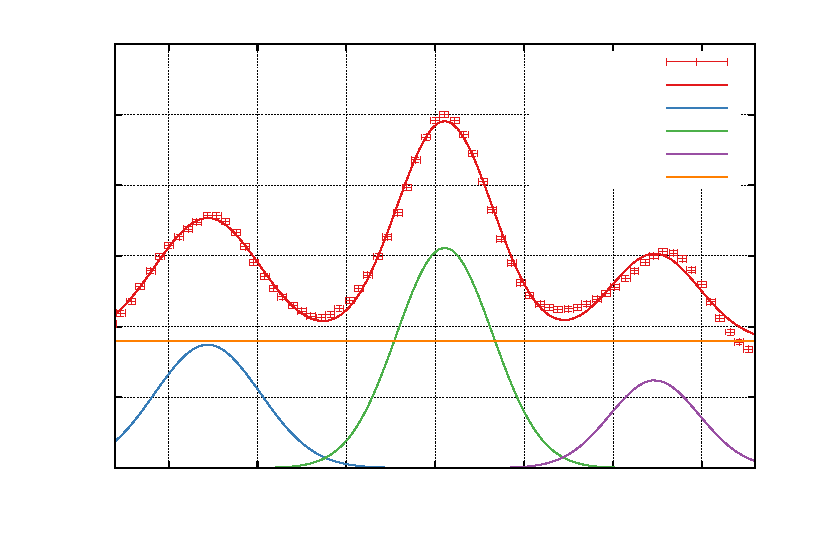
\includegraphics{./plots/zeemann_aufspaltung/b8-9}}%
    \gplfronttext
  \end{picture}%
\endgroup

\caption{8.9A}
\label{fig:gauss11}
\end{figure}
>>>>>>> d82d78ce28c8d1d4cbd2e5e1756e94d7f0579840
\end{appendix}

\end{document}
